\chapter{One-dimensional finite-volume methods}
\label{chp-1d-fv}

\theoremstyle{plain}
\newtheorem{lema}{Lemma}[chapter]

\theoremstyle{plain}
\newtheorem{prop}{Proposition}[chapter]

\theoremstyle{plain}
\newtheorem{thrm}{Theorem}[chapter]

\theoremstyle{plain}
\newtheorem{remark}{Remark}[chapter]

\theoremstyle{plain}
\newtheorem{corollary}{Corollary}[chapter]

\theoremstyle{plain}
\newtheorem{definition}{Definition}[chapter]


The aim of this chapter is to give a detailed description of the celebrated
Piecewise-Parabolic Method (PPM) proposed by \citet{colella:1984}.
As we shall see, the PPM is a one-dimensional finite-volume method for
hyperbolic conservation laws that at each time step requires two tasks. 
The first task may be stated as: given the estimates of average values of the
conservation laws solution, find a Piecewise-Parabolic function that approximates 
the function and preserves its local integral value (also referred as local mass).
The second task is the following: given the Piecewise-Parabolic approximation 
(also known as reconstruction), solve the conservation law using the parabolas 
to obtain the solution at the next time-step.
For instance, if the conservation law is the advection equation, the second step
consists of advecting the parabolas.
In the first step, we may also require some monotonization constraints on the parabolas,
to ensure that no new extreme value is created in the Piecewise-Parabolic reconstruction, 
ensuring that the scheme is free of numerical oscillations.
The steps required for PPM make it an REA (reconstruct, evolve, and average) algorithm,
or also referred to as a Godonuv-type method, which was originally proposed by 
\citet{godunov:1959}.

The PPM approach has become popular in the literature for gas 
dynamics simulations, astrophysical phenomena modeling \citep{woodward:1986}
and later on atmospheric simulations \citep{carpenter:1990}.
Indeed, the PPM has been implemented in the FV3 dynamical core on its 
latitude-longitude grid \citep{lin:2004} and cubed-sphere \citep{putman:2007}
versions.
We point out that the reconstruction function may be built using other basis 
functions rather than parabolas. In fact, PPM may be thought of as an extension of 
the Piecewise-Linear method from \citet{vanleer:1977}, which, on the other hand,
was inspired by the Piecewise-Constant method attributed to \citet{godunov:1959}.
Besides that, other schemes inspired by PPM were proposed in the literature using
higher-order polynomials, such as quartic polynomials \citep{white:2008}.
For a review of general piecewise-polynomial reconstruction we refer 
to the technical report from \citet{engwirda:2016}, \citet{lauritzen:2011}
and the references therein.
Even though many other shapes for the basis functions are available in the 
literature, as well higher order schemes, \citet{harris:2021} points out that the PPM
scheme suits well the FV3 needs in the sense of being a flexible method 
that can be modified to ensure low diffusivity or shape-preservation, for example.
Besides that, a finite-volume numerical method usually requires
monotonicity constraints, which by Godunov's theorem, limits 
the order of convergence to at most 1.
Thus, a higher-order scheme needs to be well-balanced on the trade-off between 
computational cost increasing and potential benefits.


This chapter starts with a basic review of one-dimensional conservation laws in
the integral form in Section \ref{chp2-sec1}, and in Section \ref{chp2-sec2} 
we set the framework of general one-dimensional finite-volumes schemes,
where we also introduce concepts such as consistency, convergence and stability.
Section \ref{chp2-sec-ppm} describes the PPM method and its convergence order analysis
of its reconstruction in given in Subsection \ref{chp2-sec-recon}.
Subsection \ref{chp2-sec-mono} is dedicated to introducing possible ways to monotonize
the parabolas.
Subsection \ref{chp2-sec-flux} is dedicated to the description and investigation of the PPM flux
computation considering the one-dimensional advection equation as the conservation law.
Section \ref{chp2-sec-numerical-exp} shows some numerical results using the PPM scheme
for the advection equation.  At last, Section \ref{chp2-sec-conclusion} presents
some conclusions.
The usage of PPM to solve two-dimensional problems
will be addressed in Chapter \ref{chp-2d-fv}.

\section{One-dimensional conservation law in integral form}
\label{chp2-sec1}
In this section, we are going to present the derivation of one-dimensional 
conservation laws in the integral form. 
The derivation presented here follows \citet{leveque:1990} and \citet{leveque:2002} closely and will
be useful to fix some notation. \index{Conservation law}
Let us assume that $x$ and $t$ represent the spatial and time coordinates, respectively.
Given $[x_1, x_2] \subset \mathbb{R}$, $x_1 \leq x_2$, and a time 
interval $[t_1, t_2] \subset ]0, +\infty[$, $t_1 \leq t_2$, 
we aim to describe how a state variable density given by a function
$q: \mathbb{R}\times[0, +\infty[ \to \mathbb{R}$ 
evolve within time in the considered time interval, assuming that we have neither sinks nor sources 
for the mass of the state variable and also assuming that the mass
flow rate is known.

To set the problem in more mathematical terms, let us denote by 
${q}: \mathbb{R}\times [0, +\infty[\to \mathbb{R}$, 
${q} = {q}(x,t)$, the state variable.
The mass of ${q}$ in $[x_1, x_2]$ at time $t$ is defined by:
\begin{equation}
	\label{chp2-sec1-eq1}
	{M}_{[x_1, x_2]}(t) := \int_{x_1}^{x_2} {q}(x,t) \,dx.
\end{equation}

%Thus, the mass in $[x_1, x_2]$ of the $k$-th state variable $q_k$ is equal to
%$({M}_{[x_1, x_2]}(t))_k$, $\forall k = 1, \cdots, m$.
We are going to assume the following physical constraints concerning the total mass of the state variable:
\begin{enumerate}
	\item No mass is created;
	\item No mass is destroyed.
\end{enumerate}

Also, let us assume that the mass flow rate in a point $x$ and at a time 
$t > 0$ is given by ${f}({q}(x,t))$, where ${f}:\mathbb{R} \to \mathbb{R}$ is 
a continuously differentiable ($\mathcal{C}^1$) function. This function ${f}$ is known as flux function.
With the physical constraints that we imposed, the following equation must hold for the mass:
\begin{equation}
	\label{chp2-sec1-eq2}
	\frac{d}{dt} \bigg( \int_{x_1}^{x_2} {q}(x,t) \,dx \bigg) = 
	{f}({q}(x_1,t)) - {f}({q}(x_2,t)) .
\end{equation}
Equation \eqref{chp2-sec1-eq2} is known as a conservation law written in integral form and tell us how the mass 
${M}_{[x_1, x_2]}(t)$ varies with time. Another integral form of the conservation law may be obtained integrating
Equation \eqref{chp2-sec1-eq2} with respect to time in $[t_1, t_2]$ leading to: \index{Conservation law !in integral form}
\begin{equation}
	\label{chp2-sec1-eq3}
	\int_{x_1}^{x_2} {q}(x, t_2) \,dx = 
	\int_{x_1}^{x_2} {q}(x, t_1) \,dx + 
	\int_{t_1}^{t_2} {f}({q}(x_1, t)) \,dt -
	\int_{t_1}^{t_2}{f}({q}(x_2, t)) \,dt .
\end{equation}

Assuming that ${q}$ is a $\mathcal{C}^1$ function, we may write:
\begin{equation}
	\label{chp2-sec1-eq4}
	\int_{t_1}^{t_2} 
	\frac{\partial q}{\partial t}(x,t) \,dt
	= {q}(x, t_2) - {q}(x, t_1) ,
\end{equation}
and
\begin{equation}
	\label{chp2-sec1-eq5}
	\int_{x_1}^{x_2} \frac{\partial f}{\partial x}({q}(x,t)) \,dx 
	= {f}({q}(x_2, t)) -
	{f}( {q}(x_1, t)) .
\end{equation}

Replacing Equations \eqref{chp2-sec1-eq4} and \eqref{chp2-sec1-eq5}
in \eqref{chp2-sec1-eq3} we get the differential form of the conservation law:
\index{Conservation law !in differential form}
\begin{equation}
	\label{chp2-sec1-eq6}
	\int_{t_1}^{t_2} \int_{x_1}^{x_2} 
	\bigg( \frac{\partial q}{\partial t}(x, t) 
	+ \frac{\partial f}{\partial x}({q}(x, t)) \bigg) 
	\,dx \,dt  = 0.
\end{equation}

Since Equation \eqref{chp2-sec1-eq6} must hold for all $x_1, x_2, t_1$ and $t_2$ such that
$[x_1, x_2] \times [t_1, t_2] \subset \mathbb{R}\times ]0, +\infty[$, we obtain the differential form of the conservation law:
\begin{equation}
	\label{chp2-sec1-eq7}
	\frac{\partial q}{\partial t}(x, t) +
	\frac{\partial f}{\partial x} ({q}(x, t))
	= 0, \quad \forall (x,t) \in \mathbb{R}\times ]0, +\infty[. 
\end{equation}

%We shall assume that the eigenvalues of the Jacobian matrix of the flux function
%$D{f}(q)$ are all real and that $D{f}(q)$ is a diagonalizable matrix,
%$\forall q \in \mathbb{R}^m$, so that 
Equation \eqref{chp2-sec1-eq7}
is a hyperbolic partial differential equation \citep{leveque:1990}. As we will 
specify latter, some initial conditions will also be supposed to be known as well.

Many physically relevant equations may be written as Equation \eqref{chp2-sec1-eq7}.
%Some examples are the Euler equations for gas dynamics, obtained when $m = 3$,
%and the one-dimensional shallow-water equations, obtained $m = 2$.
For instance, the Burgers equation, which is obtained when
$m = 1$ and $f(q) = q^2$. The Burgers equation is well known for developing shocks,
even for smooth initial conditions, and is a simple prototype to study shock formation.
The linear advection equation is another interesting example, which is obtained
when $m = 1$ and $f(q(x,t)) = u(x,t)q(x,t)$, where $u(x,t)$ is a given velocity.
Strictly speaking, the linear advection is not in the form given by the Equation
\eqref{chp2-sec1-eq7} since $f$ depends on $q$ but also on $(x,t)$.
But, one may check that Equation \eqref{chp2-sec1-eq7} is still hyperbolic
in this case. The linear advection equation will play a key role in this work due to its importance
to the development of atmospheric dynamical cores.

We say that ${q}$ is a strong or classical solution to the conservation law \eqref{chp2-sec1-eq7}
if it is $\mathcal{C}^1$ and satisfies the Equation \eqref{chp2-sec1-eq7}.
Applying the steps from Equation \eqref{chp2-sec1-eq3} to Equation \eqref{chp2-sec1-eq7}
in reverse order, one may check that if ${q}$ is a strong solution,
then it satisfies the integral form \eqref{chp2-sec1-eq3} for all $x_1, x_2, t_1$ and $t_2$ such that
$[x_1, x_2] \times [t_1, t_2] \subset \mathbb{R}\times ]0, +\infty[$. 
Therefore, Equations \eqref{chp2-sec1-eq3} and \eqref{chp2-sec1-eq7} are
equivalent when ${q}$ is $\mathcal{C}^1$.
However, the problem \eqref{chp2-sec1-eq3} can be formulated
to functions that are not $\mathcal{C}^1$ and have discontinuities.
More generally speaking, we say that ${q}$ is a weak solution 
if it satisfies the Equation 
\eqref{chp2-sec1-eq3} for all $x_1, x_2, t_1$ and $t_2$ such that
$[x_1, x_2] \times [t_1, t_2] \subset \mathbb{R}\times ]0, +\infty[$.
Of course $q$ and $u$ must be such that all the integrals in Equation 
\eqref{chp2-sec1-eq3} makes sense. Later (Problem \ref {chp2-sec2-prob1}), we specify the spaces where $q$ and $u$ belong.
It can be shown that this notion of weak solution is equivalent to requiring that \citep{leveque:1990}:
\begin{equation}
	\label{chp2-sec1-eq8}
	\int_{-\infty}^{+\infty} \int_{0}^{+\infty} \bigg(
	\frac{\partial \phi}{\partial t} (x, t){q}(x, t) +
	\frac{\partial \phi}{\partial x} (x ,t){f}({q}(x, t)) 
	\bigg)\,dt \,dx = 
	\int_{-\infty}^{+\infty} \phi(x, 0){q}(x, 0) \,dx  , \quad
\end{equation}
$\forall \phi \in C_{0}^{1}(\mathbb{R}\times[0, +\infty[)$
where $C_{0}^{1}(\mathbb{R}\times[0, +\infty[)$ denotes the set
of all continuously differentiable functions with compact support 
in $\mathbb{R}\times[0, +\infty[$. This formulation of weak solution
is more commonly employed in the construction of Discontinuous Galerkin
methods \citep{nair:2011}.

In order to develop finite-volume methods for a conservation law, it is useful to define the
average value of the state variable ${q}$ in the interval $[x_1, x_2]$ at a time $t$ by:
\begin{equation}
	\label{chp2-sec1-eq9}
	{Q}(t) = \frac{1}{\Delta x}
	\int_{x_1}^{x_2} {q}(x,t) \,dx,
\end{equation}
where $\Delta x = x_2 - x_1$. The Equation \eqref{chp2-sec1-eq2} may be  rewritten in terms of ${Q}$ as:
\begin{equation}
        \label{chp2-sec1-eq10}
	\frac{dQ}{dt} (t) = \frac{1}{\Delta x} 
	({f}({q}(x_1,t)) - {f}({q}(x_2,t))) ,
\end{equation}
and so is Equation \eqref{chp2-sec1-eq3}:
\begin{equation}
        \label{chp2-sec1-eq11}
	{Q}(t_2) =  {Q}(t_1) + 
	\frac{1}{\Delta x}\bigg( \int_{t_1}^{t_2} 
	{f}({q}(x_1, t)) \,dt - 
	\int_{t_1}^{t_2}{f}({q}(x_2, t)) \,dt \bigg).
\end{equation}

To move towards finite volume schemes, we will restrict our attention
to a conservation law in a bounded domain of the form 
$D = [a,b]\times[0,T]$, $a<b$, $T>0$. However, we must 
impose some boundary conditions. One possible way that we will adopt 
in the text are the periodic boundary conditions:
\begin{equation}
	\label{chp2-sec1-eq12}
	{q}(a, t) = {q}(b, t),\quad \forall t \in [0, T].
\end{equation}

Also, we assume that an initial condition $q_0(x) = q(x,0)$ is given.
Thus, we have specified a Cauchy problem.
We notice that Equations \eqref{chp2-sec1-eq10} and \eqref{chp2-sec1-eq11}
hold for all $x_1, x_2, t_1$ and $t_2$ such that
$[x_1, x_2] \times [t_1, t_2] \subset D$.
So, let us discretize the domain $D$ and write 
Equations \eqref{chp2-sec1-eq10} and \eqref{chp2-sec1-eq11} in terms of this discretization.
Given a positive integer $N_T$, we define the time step 
$\Delta t = \frac{T}{N_T}$, $t^{n} = n \Delta t$, for $n = 0, 1 ,\cdots, N_T$.
For the spatial discretization, we consider a uniformly spaced partition of $[a, b]$ given by: 
\begin{equation}
	\label{chp2-sec1-eq13}
	[a,b] = \bigcup_{i=1}^N X_i, 
	\text{ where } X_i= [x_{i-\frac{1}{2}}, x_{i+\frac{1}{2}}] \text{ and } 
	a = x_{\frac{1}{2}} < x_{\frac{3}{2}} < \cdots < x_{N-\frac{1}{2}} < x_{N+\frac{1}{2}} = b.
\end{equation}

Each interval $X_i$ is referred to as the control volume. \index{Control volume}
We shall use the notations $\Delta x = x_{i+\frac{1}{2}} - x_{i-\frac{1}{2}}$ 
and $x_i = \frac{1}{2}(x_{i+\frac{1}{2}} + x_{i-\frac{1}{2}})$, $\forall i = 1, \cdots, N$, 
to define the control volume length and centroid, respectively.
We also denote by ${Q}_i(t)$ as the
average values of state variable at time $t$
in the control volume $X_i$, $\forall i = 1, \cdots, N$. Replacing $t_1, t_2, x_1$ and 
$x_2$ by $t^{n}, t^{n+1}, x_{i-\frac{1}{2}}$ and $x_{i+\frac{1}{2}}$,
respectively, in Equation \eqref{chp2-sec1-eq10}, we get:
\begin{equation}
	\label{chp2-sec1-eq14}
	\frac{dQ_i}{dt} (t) = \frac{1}{\Delta x}
	({f}({q}(x_{i-\frac{1}{2}},t)) -
	{f}({q}(x_{i+\frac{1}{2}},t))) ,
	\quad \forall i = 1, \cdots, N.
\end{equation}
Similarly, Equation \eqref{chp2-sec1-eq11} becomes:
\begin{equation}
        \label{chp2-sec1-eq15}
	\begin{aligned}
		{Q}_i(t^{n+1}) =  {Q}_i(t^{n}) +
		\frac{1}{\Delta x}\bigg( \int_{t^{n}}^{t^{n+1}}
        	{f}({q}(x_{i-\frac{1}{2}}, t)) \,dt -
		\int_{t^{n}}^{t^{n+1}}{f}({q}(x_{i+\frac{1}{2}}, t)) \,dt \bigg),
       		\\
		\quad \forall i = 1, \cdots, N,
		\quad \forall n = 0, \cdots, N_T-1.
	\end{aligned}
\end{equation}
In order to use a more compact notation, it is helpful to use the following centered difference notation:
\begin{equation}
	\label{chp2-sec1-eq16}
	\delta_x {g}(x_i,t) = 
	{g}(x_{i+\frac{1}{2}},t) - 
	{g}(x_{i-\frac{1}{2}},t),
\end{equation}
for an arbitrary vector valued function ${g}$. 
Using this notation, Equations \eqref{chp2-sec1-eq14}
and \eqref{chp2-sec1-eq15} lead to:
\begin{equation}
        \label{chp2-sec1-eq17}
        \frac{dQ_i}{dt}(t) = -\frac{1}{\Delta x}
	\delta_x {f}({q}(x_{i},t))
        \quad \forall i = 1, \cdots, N,
\end{equation}
and
\begin{equation}
        \label{chp2-sec1-eq18}
        {Q}_i(t^{n+1}) =  {Q}_i(t^{n}) -
	\frac{\Delta t}{  \Delta x} \delta _x\bigg( \frac{1}{\Delta t}\int_{t^{n}}^{t^{n+1}}
        {f}({q}(x_{i}, t)) \,dt \bigg),
        \quad \forall i = 1, \cdots, N,
        \quad \forall n = 0, \cdots, N_T-1,
\end{equation}
respectively.
It is worth pointing out that we have made no approximation in Equations
\eqref{chp2-sec1-eq17} and \eqref{chp2-sec1-eq18}. Indeed, if ${q}$ satisfies Equation
$\eqref{chp2-sec1-eq2}$, $\forall [x_1, x_2] \subset [a,b]$ and $\forall t \in [0,T]$,
then Equation \eqref{chp2-sec1-eq17} is just Equation
\eqref{chp2-sec1-eq2} evaluated in the control volumes and written
in terms of the average values ${Q}$. 
Similarly, if ${q}$ satisfies Equation
$\eqref{chp2-sec1-eq3}$, $\forall [x_1, x_2] \times [t_1, t_2] \subset D$,
then Equation \eqref{chp2-sec1-eq18} is just Equation
\eqref{chp2-sec1-eq3} evaluated in the control volumes,
at the time instants $t^{n}$, and written
in terms of the average values ${Q}$.

Notice that in Equation \eqref{chp2-sec1-eq18} we divided and multiplied by $\Delta t$, so that 
we can interpret $\frac{1}{\Delta t}\int_{t^{n}}^{t^{n+1}}
{f}({q}(x_{i}, t)) \,dt $ as a time-averaged flux.
This interpretation is very handy for the derivation of finite-volume schemes.

The formulations given by Equations \eqref{chp2-sec1-eq17} and \eqref{chp2-sec1-eq18} are the cornerstone 
of the development of finite volume methods for conservation laws. 
On the right-hand side of Equation \eqref{chp2-sec1-eq17}, the flux function ${f}$ 
may be discretized leading to an ordinary differential equation (ODE)
that might be solved using classical ODE integrators.
These methods are known as semi-discrete methods \citep{leveque:2002}, since only the spatial coordinate is discretized.
In this work, we shall restrict our attention to methods based on Equation \eqref{chp2-sec1-eq18},
even though the PPM approach is applicable for semi-discrete methods (\textit{e.g.} \ \citet{suresh:1997}).

\section{The finite-volume approach}
\label{chp2-sec2}
We summarize the problem of the system of conservation laws in the integral form 
discussed in Section \ref{chp2-sec1} in Problem \ref{chp2-sec2-prob1}.
For simplicity, hereafter we shall constrain our attention to the one-dimensional advection equation, 
that is, we are going to assume that the flux function has the form 
$f(q(x,t)) = u(x,t)q(x,t)$, where $u(x,t)$ is the velocity which is assumed to be given.

Since we are going to consider periodic boundary conditions, it is useful to introduce some
spaces of periodic functions of period $b-a$. We are going to use the notation $\mathbb{S}^1=[a,b]$
to represent the interval that we are interested. 
This notation is justified by thinking of periodic functions as functions defined on the circle of length $b-a$.
Whenever we use the notation $\mathbb{S}^1$, $a$ and $b$ will be implicitly defined.
With that said, we define:
\begin{align*}
	\mathcal{F}(\mathbb{S}^1) &= \{q:\mathbb{R} \to \mathbb{R};\quad q(x+b-a) = q(x), \quad \forall x \in \mathbb{R}\},\\
	\mathcal{F}(\mathbb{S}^1_{T}) &= \{q:\mathbb{R}\times[0,T]\to \mathbb{R};\quad q(\cdot,t) \in \mathcal{F}(\mathbb{S}^1), \quad \forall t \in [0,T]\},\\
	\mathcal{C}^k(\mathbb{S}^1_{T}) &= \{q\in \mathcal{C}^k(\mathbb{R}\times[0,T]): q \in \mathcal{F}(\mathbb{S}^1_{T})\}.
\end{align*}
where we are using the notation $\mathbb{S}^1_{T} = \mathbb{S}^1\times[0,T]$. 
We also introduce the following the locally integrable periodic functions:
\begin{align*}
	L^p_{\text{loc}}(\Omega) &= \{q:\Omega\to \mathbb{R};\quad \int_{K} |q(x)|^p\,dx < +\infty, \quad \text{for all compact sets } K \subset \Omega\},\\
	{L}^{p}_{\text{loc}}(\mathbb{S}^1) &= \{q\in \mathcal{F}(\mathbb{S}^1): \quad  q \in L^p_{\text{loc}}(\mathbb{R})\},\\
	{L}^{p,x}_{\text{loc}}(\mathbb{S}^1_{T}) &= \{q\in \mathcal{F}(\mathbb{S}^1_{T}): \forall t \in [0,T], \quad q(\cdot,t) \in L^p_{\text{loc}}(\mathbb{R})\},\\
	{L}^{p,t}_{\text{loc}}(\mathbb{S}^1_{T}) &= \{q\in \mathcal{F}(\mathbb{S}^1_{T}): \forall x \in \mathbb{R},\quad q(x,\cdot) \in L^p_{\text{loc}}([0,T])\},\\
	{L}^{p,x,t}_{\text{loc}}(\mathbb{S}^1_{T}) &= {L}^{p,x}_{\text{loc}}(\mathbb{S}^1_{T}) \cap {L}^{p,t}_{\text{loc}}(\mathbb{S}^1_{T}).
\end{align*}
\subsection{Discretization of the problem}
\theoremstyle{plain} 
\newtheorem{prob}{Problem}[chapter]
\begin{prob}
	\label{chp2-sec2-prob1}
	Given an initial condition ${q}_0\in {L}^{1}_{\text{loc}}(\mathbb{S}^1) \cap {L}^{2}_{\text{loc}}(\mathbb{S}^1)$ and
	a velocity function $u \in {L}^{2,t}_{\text{loc}}(\mathbb{S}^1_{T})$,
	we would like to find a weak solution ${q} \in {L}^{1,x,t}_{\text{loc}}(\mathbb{S}^1_{T}) \cap {L}^{2,x,t}_{\text{loc}}(\mathbb{S}^1_{T})$
	of the advection equation in the integral form:
	\begin{equation*}
	        \int_{x_1}^{x_2} {q}(x, t_2) \,dx = 
       		\int_{x_1}^{x_2} {q}(x, t_1) \,dx + 
        	\int_{t_1}^{t_2} {(uq)}(x_1, t) \,dt -
		\int_{t_1}^{t_2}{(uq)}(x_2, t) \,dt ,
	\end{equation*}
	$\forall [x_1, x_2]\times[t_1, t_2] \subset [a,b] \times [0,T]$, 
	and
	${q}(x,0) = {q}_0(x)$, $\forall x \in [a,b]$.
\end{prob}
We point out that, for Problem \ref{chp2-sec2-prob1}, 
the total mass in $[a,b]$ satisfies: 
\begin{equation}
	{M}_{[a,b]}(t) = {M}_{[a,b]}(0), \quad \forall t \in [0,T].
\end{equation}
This is the conservation of total mass propriety and is highly desirable
for any numerical scheme that intends to give a robust approximation of a
conservation law solution.
In Section \ref{chp2-sec1} we introduced a version of Problem \ref{chp2-sec2-prob1}
considering a discretization of the domain $[a,b] \times [0,T]$. 
To define the discretization, we introduce the concepts of $\Delta x$-grid and $\Delta t$-temporal grid and $(\Delta x, \Delta t, \lambda)$ discretization.
\begin{definition}[$\Delta x$-grid]
	\label{chp2-def-1dgrid}
	For a given interval $[a,b]$ and a positive real number $\Delta x$ such that $\Delta x = (b-a)/N$, for some positive integer $N$,
	we say that a $N$-tuple $\mathcal{X}=(X_i)_{i=1}^N$ is a $\Delta x$-grid for $[a,b]$ if
	$X_i = [x_{i-\frac{1}{2}}, x_{i+\frac{1}{2}}]$, 
	$a = x_{\frac{1}{2}} < x_{\frac{3}{2}} < \cdots < x_{N-\frac{1}{2}} < x_{N+\frac{1}{2}} = b$,
	$\Delta x = x_{i+\frac{1}{2}}-x_{i-\frac{1}{2}}$. Each $X_i$ is called control volume or cell and
	$x_{i-\frac{1}{2}}$, $x_{i+\frac{1}{2}}$ are called edges of the control volume $X_i$.
\end{definition}
\begin{remark}
	We may define the cells $X_i$ for $i$ outside of the range $1,\cdots, N$ by 
	$X_i = [a+(i-1)\Delta x,a+i\Delta x]$.  These cells are called ghost cells.
\end{remark}
\begin{definition}[$\Delta t$-temporal grid]
	\label{chp2-def-timegrid}
	For a given interval $[0,T]$ and a positive real number $\Delta t$ such that $\Delta t = T/N_T$, for some positive integer $N_T$,
	we say that a $(N_T+1)$-tuple $\mathcal{T}=(T_n)_{n=0}^{N_T}$ is a $\Delta t$-temporal grid for $[0,T]$ if 
	$ T_n = [t^n, t^{n+1}]$, $t^{n} = n\Delta t$, $\Delta t = \frac{T}{N_T}$, $\forall n = 0, \cdots, N_T$.
\end{definition}
\begin{definition}[$(\Delta x,\Delta t, \lambda)$-discretization]
	\label{chp2-def-dxtimegrid}
	Given $[a,b]\times [0,T]$ and positive real numbers $\Delta x$ and $\Delta t$, we say that $(\mathcal{X},\mathcal{T})$ is a
	$(\Delta x, \Delta t, \lambda)-$discretization of $[a,b]\times [0,T]$ if $\mathcal{X}$ is a $\Delta x$-grid for $[a,b]$ and
	$\mathcal{T}$ is a $\Delta t$-temporal grid for $[0,T]$ and $\frac{\Delta t}{\Delta x} = \lambda$.
\end{definition}
\begin{remark}
	Whenever we mention a $\Delta x-$grid, or a $\Delta t$-temporal grid or a $(\Delta x,\Delta t, \lambda)$-discretization,
	then $X_i$, $N$, $t^n$ and $N_T$ shall be assumed implicitly defined.
\end{remark}
Now we define a discretized version of Problem \ref{chp2-sec2-prob1}  in Problem \ref{chp2-sec2-prob2}.
\begin{prob}
    \label{chp2-sec2-prob2}
	Assume the framework of Problem \ref{chp2-sec2-prob1}
    and that $(\mathcal{X},\mathcal{T})$ is a $(\Delta x, \Delta t, \lambda)$-discretization of $[a,b]\times [0,T]$.
	Since we are in the framework of Problem \ref{chp2-sec2-prob1}, it follows that:
	\begin{equation}
			\label{1d-fvexact-scheme}
				{Q}_i(t^{n+1}) =  {Q}_i(t^{n}) -
				\lambda \delta _x\bigg( \frac{1}{\Delta t}\int_{t^{n}}^{t^{n+1}}
				{(uq)}(x_{i}, t) \,dt \bigg),
				\quad \forall i = 1, \cdots, N,
				\quad \forall n = 0, \cdots, N_T-1,
	\end{equation}
	where ${Q}_i(t) = \frac{1}{\Delta x}
	\int_{x_{i-\frac{1}{2}}}^{x_{i+\frac{1}{2}}} {q}(x,t) \,dx$.
	Our problem now consists of finding the values ${Q}_i(t^{n})$, 
	$\forall i = 1, \cdots, N$, $\forall n = 0, \cdots, N_T-1$,
	given the initial values ${Q}_i(0)$, $\forall i = 1, \cdots N$.
	In other words, we would like to find the average values of ${q}$
	in each control volume $X_i$ at the considered time instants.
\end{prob}
Next, we introduce the definitions of grid functions at cell centroids and edges. 
\begin{definition}[$\Delta x$- grid function]
	\label{chp2-rmk-1d-gridfunction1}
	For a $\Delta x$-grid $\mathcal{X}$, we say that $Q$ is a $\Delta x$-grid function if $Q = (Q_1,\cdots, Q_N) \in \mathbb{R}^N$.
	We denote the space of $\Delta x$-grid functions by $\mathbb{R}^{\Delta x}$.
\end{definition}
\begin{definition}[$\Delta x$-C-grid wind]
	\label{chp2-rmk-1d-gridfunction2}
	For a $\Delta x$-grid $\mathcal{X}$, we say that $u$ is a $\Delta x$-C-grid function if $u = (u_{\frac{1}{2}}, \cdots, u_{N+\frac{1}{2}}) \in \mathbb{R}^{N+1}$.
	We denote the space of $\Delta x$-C-grid wind by $\mathbb{R}^{\Delta x+1}$.
\end{definition}
The definition of $\Delta x$-C-grid wind is based on the Arakawa grids \citep{arakawa:1977}.
Using a similar notation to \citet{engwirda:2016}, we define the $(r,s)$-stencil and a grid function evaluated on a stencil as follows.
\begin{definition}[$(r,s)$-stencil]
	\label{chp2-def-1d-stencil}
	For a $\Delta x$-grid $\mathcal{X}$, for each $i=0, \cdots, N$, we say define a $(r,s)$-stencil as
	$\mathcal{S}_{i+\frac{1}{2}} = \{i-r+1, \cdots, i-1, i,i+1, \cdots, i+s\}$.
\end{definition}
\begin{definition}[Grid function restricted to a stencil]
	\label{chp2-rmk-1d-Qstencil}
	For a $\Delta x$-grid, a $(r,s)$-stencil $\mathcal{S}_{i+\frac{1}{2}}$ and $Q$ a $\Delta x$-grid function, we define 
	$Q(\mathcal{S}_{i+\frac{1}{2}} )$ = $(Q_k)_{k \in \mathcal{S}_{i+\frac{1}{2}}}$.
\end{definition}
\begin{remark}
	When computing $Q(\mathcal{S}_{i+\frac{1}{2}} )$ , we may need values of $Q_i$ that are out of the range $1,\cdots, N$.
	In this case, we may think of $Q_{i}$ as a ghost cell value. 
	Since we are under the assumption of periodic boundary conditions, this problem
	is overcome by assuming periodicity on the grid function $Q$. 
	For instance, if for a $(3,3)-$stencil, we assume $Q_{0} = Q_{N}$, $Q_{-1} = Q_{N-1},$
	$Q_{-2} = Q_{N-2}$ and $Q_{N+1}=Q_1$, $Q_{N+2}=Q_2$, $Q_{N+2}=Q_3$. 
	The same applies for $\Delta x$-C-grid winds.
\end{remark}
\begin{remark}
	For Problem \ref{chp2-sec2-prob2}, we define the $\Delta x$-grid functions
	$q^n$ and $Q(t^n)$ , where ${q}^n_{i} = {q}(x_i, t^{n})$, $Q(t^n)_i = Q_i(t^n)$, for $n=0, \cdots, N_T$.
	We also define the $\Delta x$-C-grid wind $u^n$  where $u_{i+\frac{1}{2}}^n = u(x_{i+\frac{1}{2}},t^{n})$.
\end{remark}
Finally, we define the one-dimensional (1D) finite-volume (FV)
scheme problem as follows in Problem \ref{chp2-sec2-prob3}.
\begin{prob}[1D-FV scheme]
	\label{chp2-sec2-prob3}
	Assume the framework defined in Problem \ref{chp2-sec2-prob2}.
	The finite-volume approach of Problem \ref{chp2-sec2-prob2}
	consists of finding a scheme of the form:
        \begin{equation}
					\label{1d-fv-scheme}
		{Q}_{i}^{n+1} =  {Q}_{i}^{n} -
            \lambda \delta_i {F}_{i}^{n},
                \quad \forall i = 1, \cdots, N,
                \quad \forall n = 0, \cdots, N_T-1,
        \end{equation}
	where $\delta_i {F}_{i}^{n} = 
    {F}_{i+\frac{1}{2}}^{n} - {F}_{i-\frac{1}{2}}^{n}$
    and the ${Q}^{n} \in \mathbb{R}^{\Delta x}$ is intended to be an approximation
	of the other  ${Q}(t^{n})\in \mathbb{R}^{\Delta x}$ in some sense. We define
    ${Q}_{i}^{0} = {Q}_i(0)$ or ${Q}_{i}^{0} = {q}^{0}_{i}$. 
	The terms ${F}_{i+\frac{1}{2}}^{n} = \mathcal{F}
    (Q^{n}(\mathcal{S}_{i+\frac{1}{2}} ), \tilde{u}^n_{i+\frac{1}{2}})$ are known as numerical flux, 
    where $\mathcal{S}_{i+\frac{1}{2}}$ is a $(p,q)$-stencil, $\mathcal{F}:\mathbb{R}^{p+q}\times \mathbb{R} \to \mathbb{R}$ 
    is the numerical flux function, and it approximates
	$\frac{1}{\Delta t}\int_{t^{n}}^{t^{n+1}} 
    {(uq)}(x_{i+\frac{1}{2}}, t) \,dt $,
	$\forall i = 0, 1, \cdots, N$,
	or, in other words, it estimates the time-averaged fluxes at
    the control volume $X_i$ boundaries. The value $\tilde{u}_{i+\frac{1}{2}}^n$ is related to the time-averaged velocity
    and depends on values of $u_{i+\frac{1}{2}}^n$.
\end{prob}
\begin{remark}
	A scheme of the form from Equation \eqref{1d-fv-scheme} is referred to as a 1D-FV scheme and
	it is also known as a conservative scheme.
\end{remark}
For a 1D-FV the discrete total mass at the time-step $n$ is given by
\begin{equation*}
	M^n =  \Delta x \sum_{i=1}^N Q_i^n.
\end{equation*}
Therefore, the discrete total mass is constant for a 1D-FV scheme,
which follows from a straightforward computation:
\begin{align*}
	M^{n+1} =  \Delta x \sum_{i=1}^N Q_i^{n+1}
					= M^{n} - \Delta t  \sum_{i=1}^N (F^n_{i+\frac{1}{2}}- F^n_{i-\frac{1}{2}})
					= M^{n} - \Delta t (F^n_{N+\frac{1}{2}}- F^n_{\frac{1}{2}})
					= M^{n},
\end{align*}
where we are using that $F^n_{N+\frac{1}{2}} = F^n_{\frac{1}{2}}$, since we are assuming periodic boundary
conditions.
The numerical flux function for the PPM will be introduced in Section \ref{chp2-sec-flux}.

\subsection{Consistency and convergence}
\label{chp2-sub-CC}
Before moving to the definition of convergence, we point out an important relation
between the average values of $q$ and its value at the cell centroids.
We mentioned in Problem \ref{chp2-sec2-prob3} that the initial condition may be considered as $q_i^0$
instead of $Q_i(0)$. 
Furthermore, when analyzing the convergence of a 1D-FV scheme, we may 
want to compare $Q_i^n$ with $q_i^n$ since $Q_i(t^n)$ requires the computation of 
an analytical integral, which may be too complicated to obtain in some cases.
In the following Proposition \ref{prop-bound-centroid}, we give a simple proof
of that $q_i^n$ approximates $Q_i(t^n)$ with second order error when $q$ is twice
continuously differentiable.
\begin{prop}
	\label{prop-bound-centroid}
	If $q \in \mathcal{C}^2(\mathbb{S}_{T}^1)$, then $Q_i(t^n)-q_i^n = C_1 \Delta x^2$, where 
	$C_1 = \frac{1}{24}\frac{\partial^2 q}{\partial x^2} (\eta, t^n)$,  $\eta \in X_i$
\end{prop}
\begin{proof}
	Just apply Theorem \ref{prop-bound-midpoint1d} for the function $q(x,t^n)$.	
\end{proof}
To move towards the convergence of 1D-FV schemes, for  Problem \ref{chp2-sec2-prob3} we introduce the local truncation error (LTE hereafter)
$\tau_i^n$ following \citet{leveque:2002}:
\begin{equation}
	\label{consistency-1d-eq1}
	Q_i(t^{n+1}) = Q_i(t^n) - \lambda
	\bigg(\mathcal{F}(Q(t^n)(\mathcal{S}_{i+\frac{1}{2}}),\tilde{u}^n_{i+\frac{1}{2}})-
	\mathcal{F}(Q(t^n)(\mathcal{S}_{i-\frac{1}{2}}),\tilde{u}^n_{i-\frac{1}{2}}) \bigg) + \Delta t \tau_i^n.
\end{equation}
Notice the LTE is obtained by replacing the exact solution in Equation \eqref{1d-fv-scheme}.
Since $Q_i(t^n)$ is the exact solution of Equation \eqref{1d-fvexact-scheme}, 
the LTE may be rewritten as
\begin{align}
	\begin{split}
	\label{consistency-1d-eq2}
		\tau_{i}^n = 
		\frac{1}{\Delta x} \bigg[  \bigg( \frac{1}{\Delta t}\int_{t^{n}}^{t^{n+1}}
		{(uq)}(x_{i+\frac{1}{2}}, t) \,dt - \mathcal{F}(Q(t^n)(\mathcal{S}_{i+\frac{1}{2}} ),\tilde{u}^n_{i+\frac{1}{2}}) \bigg) +\\
		\bigg( \frac{1}{\Delta t}\int_{t^{n}}^{t^{n+1}}
		{(uq)}(x_{i-\frac{1}{2}}, t) \,dt - \mathcal{F}(Q(t^n)(\mathcal{S}_{i-\frac{1}{2}} ),\tilde{u}^n_{i-\frac{1}{2}}) \bigg)
		\bigg].
	\end{split}
\end{align}
The LTE gives a measure of how well the 1D-FV scheme approximates the integral form
of the considered conservation law. 
Another interpretation of the LTE is that the LTE gives the error obtained after applying
the scheme for a single time-step using the exact solution.
The 1D-FV scheme is said to be consistent
if the LTE converges to zero.

Given a $\Delta x-$grid and $Q \in \mathbb{R}^{\Delta x}$, we define the $p$-norm by
\begin{equation}
	\label{chp2-pnorm}
	\|Q\|_{p,\Delta x}=
	\begin{cases}
		\bigg( \sum_{i=1}^{N} |Q_i|^p \bigg)^{\frac{1}{p}} & \text{if } 1\leq p < \infty,\\
		\max_{i=1, \cdots, N}{|Q_i|} & \text{otherwise }.
	\end{cases}
\end{equation}
We the define $\tau^n = (\tau_1^n, \cdots, \tau^n_N)$, which represent the LTEs at the time-step $n$.
Now we can define consistency.
\begin{definition}[Consistency]
	\label{chp2-def-cons}
	Let us consider the framework of Problem \ref{chp2-sec2-prob3}.
	A 1D-FV scheme is said to be consistency in the $p$-norm if for any sequence of $(\Delta x^{(k)}, \Delta t^{(k)},\lambda)$-discretizations, 
	$k \in \mathbb{N}$, with $\lim_{k\to \infty }{\Delta x^{(k)}} = \lim_{k\to \infty }{\Delta t^{(k)}} = 0$, we have:
	\begin{equation*}
		\lim_{k \to \infty}\bigg[ {\max_{1\leq n\leq N_T^{(k)}}}{\|\tau^n\|_{p,\Delta x^{(k)}}} \bigg] = 0,
	\end{equation*}
	and it is said to be consistent with order $P$ in the $p-$norm if %there 
	%exists a constant 
	%$C$ that does not depend neither on $\Delta t$ nor on $\Delta x$, such that
	\begin{equation*}
		{\max_{1\leq n\leq N_T^{(k)}}}{\|\tau^n\|_{p,\Delta x^{(k)}}} = O(\Delta x^P).
	\end{equation*}
\end{definition}
From Equation \eqref{consistency-1d-eq2}, it follows that we basically need to ensure that 
the numerical flux function $\mathcal{F}$ converges to the time-averaged flux at edges
when $\Delta x \to 0$ in order to guarantee consistency.
In Section \ref{chp2-sec-flux} we shall address how the numerical flux from PPM
approximates the time-averaged flux at edges.

At last, we define the point-wise error at time-step $n$ by:
\begin{equation*}
	E_i^n = Q_i(t^n) - Q_i^n, \quad i=1, \cdots, N,
\end{equation*}
and we define the vector of errors by $E^n = (E_1^n, \cdots, E_N^n)$. 
\begin{definition}[Convergence]
	\label{chp2-def-conv}
	Let us consider the framework of Problem \ref{chp2-sec2-prob3}.
	A 1D-FV scheme is said to be convergent in the $p$-norm if for any sequence of $(\Delta x^{(k)}, \Delta t^{(k)},\lambda)$-discretizations, 
	$k \in \mathbb{N}$, with $\lim_{k\to \infty }{\Delta x^{(k)}} = \lim_{k\to \infty }{\Delta t^{(k)}} = 0$, we have:
	\begin{equation*}
		\lim_{k\to \infty}\bigg[ {\max_{1\leq n\leq N_T^{(k)}}}{\|E^n\|_{p,\Delta x^{(k)}}} \bigg] = 0,
	\end{equation*}
	and it is said to converge with order $P$ in the $p-$norm if
	%there exists a constant 
	%$C$ that does not depend neither on $\Delta t$ nor on $\Delta x$, such that
	\begin{equation*}
		{\max_{1\leq n\leq N_T^{(k)}}}{\|E^n\|_{p,\Delta x^{(k)}}} = O(\Delta x^P).
	\end{equation*}
\end{definition}
Subtracting Equation \eqref{1d-fv-scheme} from Equation \eqref{consistency-1d-eq1} we get
the following equation for the error:
\begin{align}
	\begin{split}
	\label{erroreq-1d-eq2}
		E^{n+1}_i = E^n_i -
		&\lambda
		\bigg[
			\bigg( \mathcal{F}(Q(t^n)(\mathcal{S}_{i+\frac{1}{2}} ),\tilde{u}^n_{i+\frac{1}{2}}) - \mathcal{F}(Q^n(\mathcal{S}_{i+\frac{1}{2}} ),\tilde{u}^n_{i+\frac{1}{2}}) \bigg) \\
		   &-\bigg( \mathcal{F}(Q(t^n)(\mathcal{S}_{i-\frac{1}{2}} ),\tilde{u}^n_{i-\frac{1}{2}}) - \mathcal{F}(Q^n(\mathcal{S}_{i-\frac{1}{2}} ),\tilde{u}^n_{i-\frac{1}{2}}) \bigg)
		\bigg] 
		+ \tau_{i}^n \Delta t .
	\end{split}
\end{align}
Notice that if $q,u \in \mathcal{C}^3$, we can rewrite Equation \ref{consistency-1d-eq2} as:
\begin{align*}
	\begin{split}
		\tau_{i}^n = 
		\bigg[ \frac{1}{\Delta x \Delta t}  \int_{t^{n}}^{t^{n+1}} \int_{x_{i-\frac{1}{2}}}^{x_{i+\frac{1}{2}}}
		{\frac{\partial (uq)}{\partial x}}(x, t) \,dx \,dt - 
		\bigg(\frac{\mathcal{F}(Q(t^n)(\mathcal{S}_{i+\frac{1}{2}} ),\tilde{u}^n_{i-\frac{1}{2}})) -\mathcal{F}(Q(t^n)(\mathcal{S}_{i+\frac{1}{2}} ),\tilde{u}^n_{i-\frac{1}{2}})}{\Delta x} \bigg)
		\bigg].
	\end{split}
\end{align*}
Using the midpoint rule for integration (Theorem \ref{prop-bound-midpoint1d}) and the mean value theorem for integrals
(Theorem \ref{anexo-numint-mv}), 
we have:
\begin{align}
	\begin{split}
		\label{consistency-1d-eq3}
		\tau_{i}^n 
		&= 
		\bigg[ \frac{1}{\Delta t}  \int_{t^{n}}^{t^{n+1}}
		{\bigg(\frac{\partial (uq)}{\partial x}}(x_i, t) + \frac{\Delta x^2}{24}\frac{\partial (uq)}{\partial x}(\xi, t) \bigg) \,dt - 
		\bigg(\frac{\mathcal{F}(Q(t^n)(\mathcal{S}_{i+\frac{1}{2}}),\tilde{u}^n_{i+\frac{1}{2}})) 
		-\mathcal{F}(Q(t^n)(\mathcal{S}_{i-\frac{1}{2}}),\tilde{u}^n_{i-\frac{1}{2}})}{\Delta x} \bigg)
		\bigg] \\
		& = 
		\bigg[ \frac{1}{\Delta t}  \int_{t^{n}}^{t^{n+1}}
		{\frac{\partial (uq)}{\partial x}}(x_i, t) \,dt - 
		\bigg(\frac{\mathcal{F}(Q(t^n)(\mathcal{S}_{i+\frac{1}{2}}),\tilde{u}^n_{i+\frac{1}{2}})) -\mathcal{F}(Q(t^n)(\mathcal{S}_{i-\frac{1}{2}}),\tilde{u}^n_{i-\frac{1}{2}})}{\Delta x} \bigg)
		\bigg] +  \frac{\Delta x^2}{24}\frac{\partial^3 (uq)}{\partial x^3}(\xi, \overline{t}), 
	\end{split}
\end{align}
for $\xi \in X_i$ and $\overline{t} \in [t^{n},t^{n+1}]$. Therefore, if $q,u \in \mathcal{C}^3$ the scheme is
consistent, if and only if, $\frac{1}{\Delta t}  \int_{t^{n}}^{t^{n+1}} {\frac{\partial (uq)}{\partial x}}(x_i, t) \,dt$
is approximated by 
$\frac{\mathcal{F}(Q(t^n)(\mathcal{S}_{i+\frac{1}{2}}),\tilde{u}^n_{i+\frac{1}{2}})) -\mathcal{F}(Q(t^n)(\mathcal{S}_{i-\frac{1}{2}} ),\tilde{u}^n_{i-\frac{1}{2}})}{\Delta x}$.
This shall be very useful when we consider two-dimensional schemes, where we are going to use the discrete operators to estimate the divergence
of velocity fields.

\subsection{Stability}
\label{chp2-sub-stability}
In order to define the concept of stability, it is useful to introduce an operator
representation of 1D-FV schemes.
In the context of Problem \ref{chp2-sec2-prob3}, we define the operators
$\mathcal{H}_{\Delta x,n}: \mathbb{R}^{\Delta x} \to \mathbb{R}^{\Delta x}$ whose $i$-th entry is given by:
\begin{equation}
	[\mathcal{H}_{\Delta x,n}(Q)]_i = Q_i -
	\lambda \bigg( \mathcal{F}(Q(\mathcal{S}_{i+\frac{1}{2}} ),\tilde{u}^n_{i+\frac{1}{2}}) 
	- \mathcal{F}(Q(\mathcal{S}_{i-\frac{1}{2}} ),\tilde{u}^n_{i-\frac{1}{2}}) \bigg),
\end{equation}
for $i=1, \cdots, N$, $n=0, \cdots, N_T-1$.
Notice that the dependence on $n$ is due to the velocity that may be allowed
to vary with time.
As it is usual, we are assuming periodicity in the entries of $Q$ when 
we apply the operator $\mathcal{H}_{\Delta x,n}$.
Thus, Equation \eqref{1d-fv-scheme} may be rewritten in a vector form by
\begin{equation*}
	Q^{n+1} = \mathcal{H}_{\Delta x,n}(Q^n),
\end{equation*}
and Equation \eqref{consistency-1d-eq1} in a vector form reads
\begin{equation*}
	Q(t^{n+1}) = \mathcal{H}_{\Delta x,n}(Q(t^n)) + \Delta t \tau^n,
\end{equation*}
and the error equation \eqref{erroreq-1d-eq2} is given by
\begin{equation}
	\label{erroreq-1d-eq3}
	E^{n+1} = \mathcal{H}_{\Delta x,n}(Q(t^n)) - \mathcal{H}_{\Delta x,n}(Q^n) +  \Delta t \tau^n.
\end{equation}
The stability theory focus on uniformly bounding the norm of $\mathcal{H}_{\Delta x,n}(Q(t^n)) - \mathcal{H}_{\Delta x,n}(Q^n)$ \citep{leveque:2002}.
We define stability as follows.

\begin{definition}[Stability]
	In the context of Problem  \ref{chp2-sec2-prob3},
	a 1D-FV scheme is stable in the $p-$norm if for any $(\Delta x, \Delta t, \lambda)$-discretization of $[a,b]\times [0,T]$ we have:
	\begin{equation}
		\|\mathcal{H}_{\Delta x,n}(Q) - \mathcal{H}_{\Delta x,n}(P)\|_{p,\Delta x} \leq (1+\alpha \Delta t)  \|Q-P\|_{p,\Delta x},
	\end{equation}
	for all $Q, P \in \mathbb{R}^{\Delta x}$ and $\alpha$ is a constant
	that does not depend neither on $\Delta x$ nor on  $\Delta t$.
\end{definition}
Assuming that the scheme is stable in the $p-$norm, then it follows from Equation \eqref{erroreq-1d-eq3} that:
\begin{align}
	\label{chp2-sec2-erroreq}
	\begin{split}
	\|E^{n+1}\|_{p,\Delta x} 
	&\leq \|\mathcal{H}_{\Delta x,n}(Q(t^n)) - \mathcal{H}_{\Delta x,n}(Q^n)\|_{p,\Delta x} +  \Delta t \max_{n=1, \cdots, N_T}\|\tau^n\|_{p,\Delta x}\\
	&\leq (1+\alpha \Delta t)\|E^n\|_{p,\Delta x} +  \Delta t \max_{n=1, \cdots, N_T}\|\tau^n\|_{p,\Delta x}\\
	&\leq (1+\alpha \Delta t)^n\|E^0\|_{p,\Delta x} +  \Delta t \max_{n=1, \cdots, N_T}\|\tau^n\|_{p,\Delta x}
	\sum_{k=0}^{n-1} (1+\alpha \Delta t)^k\\
  &\leq e^{\alpha T}(\|E^0\|_{p,\Delta x} + T\max_{n=1, \cdots, N_T}\|\tau^n\|_{p,\Delta x}), \\
	\end{split}
\end{align}
where we used $n \Delta t\leq T $, $T=N\Delta t$ and the inequality $e^t> 1+t$.
When computing the initial average values using the value at the cell centroid, 
the initial error $E^0$ converges to zero provided $q$ is twice continuously differentiable
by Proposition \ref{prop-bound-centroid}.
Therefore, it follows that if the scheme is stable and consistent
then it is convergent. 
Furthermore, if it is stable and consistent with order $P$, then
the convergence order is at least equal to $\min\{{P,2}\}$.
In the case where both the conservation law and $\mathcal{H}_{\Delta x,n}$ are linear,
this result is a particular case of the Lax-Ritchmyer stability and the convergence
is guaranteed by the Lax equivalence theorem \citep{leveque:2002}.
In this Chapter, we are interested only in the linear advection equation.
However, as we shall see in Section \ref{chp2-sec-flux}, the operator $\mathcal{H}_{\Delta x,n}$
may become non-linear when monotonicity constraints are activated.

Notice that, if $\mathcal{H}_{\Delta x,n}$ is linear, then stability is equivalent to require that
\begin{equation*}
	\|\mathcal{H}_{\Delta x,n}\|_{p,\Delta x} \leq 1+ \alpha \Delta t,
\end{equation*}
where
\begin{equation*}
	\|\mathcal{H}_{\Delta x,n}\|_{p,\Delta x} = \sup_{Q\in \mathbb{R}^{\Delta x}} \frac{\|\mathcal{H}_{\Delta x,n}(Q)\|_{p,\Delta x}}{\|Q\|_{p,\Delta x}},
\end{equation*}
is the operator $p$-norm.

For linear operators, we may use the discrete Fourier transform \citep{trefethen:2000}
to estimate the 2-norm of $\mathcal{H}_{\Delta x,n}$. This approach is known as Von Neumann stability analysis.
We define the nodes $\theta_i = i\frac{2\pi}{N}$, $i=1, \cdots, N$, $\Delta \theta = \frac{2\pi}{N}$,
$\theta = (\theta_1, \theta_2, \cdots, \theta_N)$.
The imaginary unit is denoted by $\imath$.
The Fourier modes are given by:
\begin{equation*}
	e^{\imath k \theta} = (e^{\imath k\theta_1}, e^{\imath k\theta_2}, \cdots, e^{\imath k\theta_N}) \in \mathbb{C}^N, 
\end{equation*}
for $k=1, \cdots, N$. 
Each $k$ is referred to wavenumber and $\theta_k$ is called  dimensionless wavenumber.
The Fourier modes form an orthogonal basis of $\mathbb{C}^N$ with respect to the 
inner product
\begin{equation*}
	\langle Q, P \rangle = \frac{1}{N}\sum_{i=1}^{N}{Q_i \overline{P_i}},
\end{equation*}
for $P, Q \in \mathbb{C}$ and $\overline{z}$ denotes the complex conjugate of $z$. 
Given $Q \in \mathbb{R}^{\Delta x}$, we may may express it in terms of the Fourier modes
\begin{equation*}
	Q = \sum_{k=1}^{N} a_k \exp(\imath k \theta),
\end{equation*}
where $a_k \in \mathbb{C}$. The 2-norm of $Q$ is then given by:
\begin{equation*}
	\|Q\|_{2,\Delta x} = \sqrt{N \sum_{k=1}^{N} |a_k|^2}.
\end{equation*}
The idea of Von Neumann stability analysis is to apply the operator $\mathcal{H}_{\Delta x,n}$ on each Fourier mode and
analyze how it modifies its amplitude.
For ease of analysis, we assume that the velocity is constant, which implies that
the operator $\mathcal{H}_{\Delta x,n}$ has constant coefficients and does not depend on $n$.
For the general case, where the velocity is not constant, the stability
can be ensured using the frozen coefficients method \citep[p.~59]{strikwerda:2004}.
This method boils down to performing multiple times the stability analysis with a constant velocity
being equal to each one of the possible values of the velocity on the grid.
If the scheme is stable for all the possible constant velocities, then stability is ensured.
Since the operator is supposed to be linear with constant coefficients and we
are assuming periodic boundaries conditions, we may write:
\begin{equation*}
	\mathcal{H}_{\Delta x,n}(e^{\imath k \theta}) = \rho(k)  e^{\imath k \theta},
\end{equation*}
where the term $\rho(k)$ is called amplification factor and it is an eigenvalue of $\mathcal{H}_{\Delta x,n}$.
The norm of $\mathcal{H}_{\Delta x,n}(Q)$ is bounded by:
\begin{equation*}
	\|\mathcal{H}_{\Delta x,n}(Q)\|_{2,\Delta x}^2 = N \sum_{k=1}^{N} |a_k|^2 |\rho(k)|^2 \leq 
	\max_{k=1, \cdots, N}{|\rho(k)|}^2 \|Q\|_{2,\Delta x}^2.
\end{equation*}
Therefore:
\begin{equation*}
	\|\mathcal{H}_{\Delta x,n}\|_{2,\Delta x} \leq \max_{k=1, \cdots, N}{|\rho(k)|}.
\end{equation*}
If we show that $\max_{k=1, \cdots, N}{|\rho(k)|} \leq 1 + \alpha \Delta t$, 
with $\alpha$ independent of $\Delta t$, $N$ and $n$, then we ensure the stability of $\mathcal{H}_{\Delta x,n}$.
Generally speaking, the numerical flux can be written as a linear function
\begin{equation*}
	\mathcal{F}(Q(\mathcal{S}_{i+\frac{1}{2}}), \tilde{u}^n_{i+\frac{1}{2}}) = \sum_{l \in \mathcal{S}_{i+\frac{1}{2}}} \alpha_{l,i} Q_{l}, 
\end{equation*}
when no monotonicity constraint is imposed, 
where the coefficients $\alpha_{l,i}$ depend on $\tilde{u}^n, \Delta t$ and $\Delta x$.
We can then express $\rho$ in terms of $\alpha_{l,i}$.
Indeed, when we apply the operator $\mathcal{H}_{\Delta x,n}$ in a Fourier mode, we get:
\begin{align*}
	\begin{split}
		[\mathcal{H}_{\Delta x,n}(e^{\imath k\theta})]_i &= e^{\imath k\theta_i} - \lambda 
		\bigg(\sum_{l \in \mathcal{S}_{i+\frac{1}{2}}} \alpha_{l,i}   e^{\imath k\theta_{l}} - 
		\sum_{l \in \mathcal{S}_{i-\frac{1}{2}}} \alpha_{l,i-1} e^{\imath k\theta_{l-1}} \bigg)\\
		&= e^{\imath k \theta_i}\bigg(1 - \lambda 
		\bigg(\sum_{l \in \mathcal{S}_{i+\frac{1}{2}}} \alpha_{l,i}   e^{\imath k\theta_{l-i}} - 
		\sum_{l \in \mathcal{S}_{i-\frac{1}{2}}} \alpha_{l,i-1} e^{\imath k\theta_{l-1-i}} \bigg) \bigg).\\
	\end{split}
\end{align*}
Hence, the amplification factor has the form
\begin{equation}
\label{chp2-amplification}
\rho(k) = 1 - \lambda
					\bigg(\sum_{l \in \mathcal{S}_{i+\frac{1}{2}}} \alpha_{l,i}   e^{\imath k\theta_{l-i}} - 
					\sum_{l \in \mathcal{S}_{i-\frac{1}{2}}} \alpha_{l,i-1} e^{\imath k\theta_{l-1-i}} \bigg).
\end{equation}
In Section \ref{chp2-sec-flux} we shall analyse $|\rho(k)|$ in terms of the PPM coefficients.


\section{The Piecewise-Parabolic Method}
\label{chp2-sec-ppm}
In this Section, we are going to review and analyze the Piecewise-Parabolic method (PPM).
This method was proposed by \citet{colella:1984} for gas dynamic simulations and
its viability for atmospheric simulations has been shown by \citet{carpenter:1990}.
This method is based on using parabolas to reconstruct the function from its 
average values, ensuring mass conservation and monotonicity.
PPM is an extension of the Piecesiwe-Linear method from \citet{vanleer:1977}
and it is employed in the FV3 model using the dimension splitting method from \citet{lin:1996}.
This section is organized as follows: in Subsection \ref{chp2-sec-recon} 
we present and analyze the PPM reconstruction method and the monotonization and 
flux computation are presented and analyzed in Subsections 
\ref{chp2-sec-mono} and \ref{chp2-sec-flux}, respectively.

\subsection{Reconstruction}
\label{chp2-sec-recon}
Let us consider a function ${q} \in L^{1}_{\text{loc}}(\mathbb{R})$, a $\Delta x$-grid 
$\mathcal{X}$ of $[a,b]$ and assume that we are given the average values ${Q}_i = \frac{1}{\Delta x} 
\int_{x_{i-\frac{1}{2}}}^{x_{i+\frac{1}{2}}} {q}(x) \,dx$
on each control volume $X_i$, $\forall i = 1, \cdots, N $. In this context, it is useful to define 
the $\Delta x$-grid function $Q=(Q_1, \cdots, Q_N) \in \mathbb{R}^{\Delta x}$.
We make use of the indicator function of each control volume $X_i$ defined by:
\begin{equation*}
	\label{chp2-sec3-1-eq1}
	\chi_{i}(x)=
	\begin{cases}
		1 & \text{if } x \in X_i\\
		0 & \text{otherwise }
	\end{cases}
\end{equation*}
Using a notation similar to \citet[Chapter~1]{stoer:2002}, 
we assume that we have a family of functions $\Phi(\xi;\mu)$ defined for $\xi \in [0,1]$ depending on
a parameter $\mu =(\mu_0, \mu_1,\cdots, \mu_d)\in \mathbb{R}^{d+1}$. 
The reconstruction problem consists of finding a piecewise function:
\begin{equation}
	\label{chp2-sec3-1-eq2}
	q_{Pd}(x;Q) = \sum_{i=1}^{N} \chi_i(x) q_i(x;Q),
\end{equation}
where $q_i(x;Q) = \Phi\big(\frac{x-x_{i-\frac{1}{2}}}{\Delta x};\alpha_i\big)$, 
$\alpha_i= (\alpha_{i0},\alpha_{i1}, \cdots \alpha_{id})\in\mathbb{R}^{d+1}$ is such that:
\begin{equation*}
	\frac{1}{\Delta x}\int_{x_{i-\frac{1}{2}}}^{x_{i+\frac{1}{2}}} {q}_{Pd}(x;Q) \,dx =
	\frac{1}{\Delta x}\int_{x_{i-\frac{1}{2}}}^{x_{i+\frac{1}{2}}} q_i(x;Q) \,dx =
	\int_{0}^{1} \Phi(\xi;\alpha_i) \,d\xi = {Q}_i,
\end{equation*}
that is, $q_i(x;Q)$ preserves the mass on each control volume $X_i$.

Notice that since $q_i(x;Q) = \Phi\big(\frac{x-x_{i-\frac{1}{2}}}{\Delta x};\alpha_i\big)$, 
it is reasonable that $\Phi(0;\alpha_i)$ should approximate $q_i(x_{i-\frac{1}{2}})$ and $\Phi(1;\alpha_i)$ should approximate $q(x_{i+\frac{1}{2}})$.
Furthermore, if $q$ and $\Phi$ are differentiable enough, then 
$\Phi^{(l)}(0;\alpha_i)$ should approximate $(\Delta x)^l q^{(l)}(x_{i-\frac{1}{2}})$ and $\Phi^{(l)}(1;\alpha_i)$ should approximate
$(\Delta x)^l q^{(l)}(x_{i+\frac{1}{2}})$, whenever these derivatives exist.
One way to estimate these values at the edges $x_{i+\frac{1}{2}}$ using the average values $Q$ is to use the reconstruction method
based on primitive functions \citep[Chapter~17]{leveque:2002}.
Observe that if we define 
\begin{equation}
\label{chp2-sec-recon-ppm-eq5}
Q(x) = \int_{a}^x q(\xi) \,d\xi,
\end{equation}
we have $Q^{(l)}(x) = q^{(l-1)}(x)$. In particular, $Q^{(l)}(x_{i+\frac{1}{2}}) = q^{(l-1)}(x_{i+\frac{1}{2}})$ and
$Q^{(l)}(x_{i+\frac{1}{2}}) = \Delta x\sum_{k=1}^i Q_k$, $\forall i=0, \cdots, N$.
Therefore we can use finite-difference schemes to estimate $q^{(l-1)}(x_{i+\frac{1}{2}})$
using the $\Delta x$-grid function $Q$, once this one is assumed to be given.
Let us assume that the $l-$th derivative of $Q$ at $x_{i+\frac{1}{2}}$ is approximated using
a stencil $\mathcal{S}^{(l)}_{i+\frac{1}{2}}$ and weights $\beta^{(l)}_{k,i}$, $k \in \mathcal{S}^l_{i+\frac{1}{2}}$.
If $d$ is odd, then we may search for a parameter $\alpha_i \in \mathbb{R}^{d+1}$ that ensures mass conservation and approximation of 
$q$ and its derivatives at edges by solving:
\begin{equation}
	\label{chp2-recon-sys1}
	\begin{cases}
		\int_{0}^{1} \Phi(\xi;\alpha_i) \,d\xi &= {Q}_i,\\
		\Phi^{(l)}(0;\alpha_i) &= (\Delta x)^l \sum_{k \in \mathcal{S}^{(l)}_{i-\frac{1}{2}}} \beta_{k,i}^{(l)} {Q}_k, \quad \text{for } l = 0, \cdots, d-1.
	\end{cases}
\end{equation}
If $d$ is even, similarly we look for a parameter $\alpha_i \in \mathbb{R}^{d+1}$ that solves:
\begin{equation}
	\begin{cases}
		\label{chp2-recon-sys2}
		\int_{0}^{1} \Phi(\xi;\alpha_i) \,d\xi &= {Q}_i,\\
		\Phi^{(l)}(0;\alpha_i) &= (\Delta x)^l \sum_{k \in \mathcal{S}^{(l)}_{i-\frac{1}{2}}} \beta_{k,i}^{(l)} {Q}_k, \quad \text{for } l = 0, \cdots, \frac{d}{2}-1,\\
		\Phi^{(l)}(1;\alpha_i) &= (\Delta x)^l \sum_{k \in \mathcal{S}^{(l)}_{i+\frac{1}{2}}} \beta_{k,i}^{(l)} {Q}_k, \quad \text{for } l = 0, \cdots, \frac{d}{2}-1.
	\end{cases}
\end{equation}
The reconstruction problem is linear if $\Phi(\xi;\mu)$ may be expressed as:
\begin{equation*}
	\Phi(\xi;\mu) = \sum_{k=0}^d \mu_k \Phi_k(\xi),
\end{equation*}
for functions $\Phi_k$ defined on $[0,1]$. In this case, Equation \eqref{chp2-recon-sys1} and  Equation \eqref{chp2-recon-sys2}
are $(d+1)\times (d+1)$ linear systems.
It is usually common to assume that $\Phi_k$'s are linearly independent.
Thus, we have described a method that allows us to reconstruct a function from its average values
preserving its mass in each control value and approximates $q$ at the edges that, in principle,
works for functions $\Phi_k$ provided they are differentiable enough.
For instance, we could choose $d=0$, and $\Phi_0(\xi)=1$. 
In this case, we have piecewise constant functions as used in \citet{godunov:1959}.
If we choose $d=1$, $\Phi_0(\xi)=1$ and $\Phi_1(\xi)=\xi$, 
we have a piecewise linear reconstruction as in \citet{vanleer:1977}. 
For further polynomial reconstruction schemes, we refer to \citet{engwirda:2016} and the references therein.

Hereafter, we are going the focus on the piecewise parabolic method from \citet{colella:1984} that uses $d=2$, 
$\Phi_0(\xi)=1$, $\Phi_1(\xi)=\xi$, $\Phi_1(\xi)=(1-\xi)\xi$. 
In this case, we denote $q_{Pd}$ by $q_{PP}$.
In order to follow the notation from \citet{colella:1984},
we write $\alpha_{0i} = q_{L, i}$, $\alpha_{1i} = \Delta q_i$ and $\alpha_{2i} = q_{6, i}$.
Therefore, each $q_i$ may be expressed as:
\begin{equation}
	\label{chp2-sec-recon-ppm-eq1}
	q_i(x;Q) = q_{L, i} + \Delta q_i z_i(x) + q_{6, i}z_i(x)(1-z_i(x)), 
	\quad \text{where }
	z_i(x) = \frac{x-x_{i-\frac{1}{2}}}{\Delta x},
	\quad x \in X_i,
\end{equation}
where the values $q_{L, i}$, $\Delta q_i$ and $q_{6, i}$  will be specified latter.
Note that each $z_i$ is just a normalization function that maps $X_i$ onto $[0,1]$.
It is easy to see that 
$\lim_{x \to x_{i-\frac{1}{2}}^+} {q_i(x;Q)} = q_{L, i}$.
If we define $q_{R, i} = \lim_{x \to x_{i+\frac{1}{2}}^-} {q_i(x;Q)}$,
then we have:
\begin{equation}
	\label{chp2-sec-recon-ppm-eq2}
	\Delta q_i = q_{R, i} - q_{L, i}.
\end{equation}
The average value of $q_i$ is given by:
\begin{equation}
	\label{chp2-sec-recon-ppm-eq3}
	\frac{1}{\Delta x}\int_{x_{i-\frac{1}{2}}}^{x_{i+\frac{1}{2}}} {q}_i(x;Q) \,dx
	= \frac{(q_{L,i} + q_{R,i})}{2} + \frac{q_{6,i}}{6}.
\end{equation}
Under the hypothesis of mass conservation, we have:
\begin{equation}
	\label{chp2-sec-recon-ppm-eq4}
	q_{6,i} = 6\bigg(Q_i - \frac{(q_{L,i} + q_{R,i})}{2}\bigg).
\end{equation}
Therefore, we have found the parameters $\Delta q_i$ and $q_{6, i}$ as
functions of the parameters $q_{L, i}$ and $q_{R, i}$,
such that the parabola $q_i$ from \eqref{chp2-sec3-1-eq2} 
guarantees mass conservation. To completely determine the 
parabola $q_i$, we need to set the values $q_{L, i}$ and
$q_{R, i}$, which, as we have seen, represent the limits of $q_i$ when
$x$ tends to the left and right boundaries of $X_i$, respectively.
Hence, it is natural to seek for $q_{L, i}$ as an approximation of $q(x_{i-\frac{1}{2}})$
and $q_{R, i}$ as an approximation of $q(x_{i+\frac{1}{2}})$.
As we mentioned before in after introducing Equation \eqref{chp2-sec-recon-ppm-eq5}, this is achieved
using finite-differences.
An explicit expression for the approximation of $q(x_{i-\frac{1}{2}})$, denoted by $q_{i+\frac{1}{2}}$, is given by \citep{colella:1984}:
\begin{equation}
	\label{chp2-sec-recon-ppm-eq7}
	q_{i+\frac{1}{2}} = \frac{1}{2} \bigg( Q_{i+1} + Q_{i} \bigg) - \frac{1}{6} \bigg( \delta Q_{i+1} - \delta Q_{i}\bigg),
\end{equation}
where $\delta Q_{i}$ is the average slope in the $i$-th control-volume:
\begin{equation}
	\label{chp2-sec-recon-ppm-eq8}
	\delta Q_{i} = \frac{1}{2} \bigg( Q_{i+1} - Q_{i-1} \bigg).
\end{equation}
We notice that Formula \eqref{chp2-sec-recon-ppm-eq8} may be rewritten more explicitly as:
\begin{equation}
	\label{chp2-sec-recon-ppm-eq9}
	q_{i+\frac{1}{2}} = \frac{7}{12} \bigg( Q_{i+1} + Q_{i} \bigg) - \frac{1}{12} \bigg(  Q_{i+2} +Q_{i-1}\bigg).
\end{equation}
The Formula \eqref{chp2-sec-recon-ppm-eq9} is fourth-order accurate if
$q$ is at least $\mathcal{C}^4$ \citep{colella:1984}. Indeed, we
prove this later in Proposition \ref{prop:ppm-bound1}.
An explicit expression for the values of $q_{R,i}$ and $q_{L,i}$ are given by:
\begin{align}
	\label{chp2-sec-recon-ppm-eq10}
	q_{R,i} = q_{i+\frac{1}{2}} = \frac{7}{12} \bigg( Q_{i+1} + Q_{i} \bigg) - \frac{1}{12} \bigg(  Q_{i+2} +Q_{i-1}\bigg), \\
	\label{chp2-sec-recon-ppm-eq11}
	q_{L,i} = q_{i-\frac{1}{2}} = \frac{7}{12} \bigg( Q_{i} + Q_{i-1} \bigg) - \frac{1}{12} \bigg(  Q_{i+1} +Q_{i-2}\bigg).
\end{align}
We point out that a fifth-order accurate for the values of $q_{R,i}$ and $q_{L,i}$
is also possible, as it was developed by \citet{putman:2007} 
based on the work \citet{suresh:1997}. The fifth-order reconstruction formula reads:
\begin{align}
	\label{chp2-sec-recon-ppm-eq12}
	q_{R,i} &= \frac{1}{60} \bigg( 2Q_{i-2} - 13Q_{i-1} + 47Q_{i} + 27Q_{i+1} - 3Q_{i+2}\bigg), \\
	\label{chp2-sec-recon-ppm-eq13}
	q_{L,i} &= \frac{1}{60} \bigg(-3Q_{i-2} + 27Q_{i-1} + 47Q_{i} - 13Q_{i+1} + 2Q_{i+2}\bigg).
\end{align}
However, we notice that this reconstruction scheme allows discontinuity of the 
Piecewise-Parabolic function at the control volume edges since the stencil it is not symmetric.

\subsubsection{PPM reconstruction order analysis}
\label{chp2-sec-numerical-analysis}
As we pointed out before, the approximation of $q$ at the control volumes edges
given by Equation \eqref{chp2-sec-recon-ppm-eq9} is fourth-order accurate when $q \in \mathcal{C}^4(\mathbb{R})$. 
This is proved as a Corollary of the following Proposition \ref{prop:ppm-bound1}.
\begin{prop}
	\label{prop:ppm-bound1}
	Let $q \in \mathcal{C}^{4}(\mathbb{R})$, $\overline{x} \in \mathbb{R} $ and $h>0$.
	Then, the following identity holds:
	\begin{equation}
		\label{prop:ppm-bound1-eq1}
		q(\overline{x} ) = \frac{7}{12}\bigg( \frac{1}{h} \int_{\overline{x} }^{\overline{x}+h} q(x) \,dx 
		       + \frac{1}{h} \int_{\overline{x} -h}^{\overline{x} } q(x) \,dx  \bigg)
		       - \frac{1}{12}\bigg( \frac{1}{h} \int_{\overline{x} +h}^{\overline{x}+2h} q(x) \,dx 
		       + \frac{1}{h} \int_{\overline{x} -2h}^{\overline{x} -h} q(x) \,dx  \bigg) + C_1h^4,
	\end{equation}
	where $C_1$ is a constant that depends on $q$ and $h$.
\end{prop}
\begin{proof}
	We define $Q(x) = \int_{a}^{x} q(\xi) \,d\xi$ for fixed $a \in \mathbb{R}$ as in 
	Equation \eqref{chp2-sec-recon-ppm-eq5}. It follows that:
	\begin{align*}
		\int_{\overline{x}}^{\overline{x}+h} q(\xi) \,d\xi + \int_{\overline{x}-h}^{\overline{x}} q(\xi) \,d\xi &=
		Q(\overline{x}+h) - Q(\overline{x}-h), \\
		\int_{\overline{x}+h}^{\overline{x}+2h} q(\xi) \,d\xi + \int_{\overline{x}-2h}^{\overline{x}-h} q(\xi) \,d\xi &=
		Q(\overline{x}+2h) - Q(\overline{x}-2h) - (Q(\overline{x}+h) - Q(\overline{x}-h)). \\
	\end{align*}
	Using these identities, Equation \eqref{prop:ppm-bound1-eq1} may be rewritten as:
	\begin{equation}
		\label{prop:ppm-bound1-eq2}
		q(\overline{x}) = \frac{4}{3} \bigg(\frac{Q(\overline{x}+h) - Q(\overline{x}-h)}{2h}\bigg)
		       - \frac{1}{3} \bigg(\frac{Q(\overline{x}+2h) - Q(\overline{x}-2h)}{4h}\bigg) + C_1h^4,
	\end{equation}
	which consists of finite-difference approximations. 
	Thus, Equation \eqref{prop:ppm-bound1-eq1} follows from Lemma \ref{lemma:fd-ppm-est1}
	with:
	\begin{equation}
		\label{prop:ppm-bound1-eq3}
		C_1 = C_1(\mu_1,\mu_2) = \frac{1}{720}\bigg(6q^{(4)}(\mu{1}) -32q^{(4)}(\mu_{2})\bigg), 
	\end{equation}
	where $\mu_{1}, \mu_{2} \in [\overline{x}-2h,\overline{x}+2h]$,
	which concludes the proof.
\end{proof}
\begin{corollary}
	\label{prop:ppm-bound1-corollary}
	It follows from Proposition \ref{prop:ppm-bound1} with
	$\overline{x} = x_{i+\frac{1}{2}}$ and $h = \Delta x$
	that $q_{i+\frac{1}{2}}$ given by Equation \eqref{chp2-sec-recon-ppm-eq9} satisfies:
	\begin{equation}
		\label{ppm-edges-bound1}
		q{(x_{i+\frac{1}{2}})} - q_{i+\frac{1}{2}} = C_1\Delta x^4,
	\end{equation}
	with $C_1$ given by Equation \eqref{prop:ppm-bound1-eq3}, whenever $q \in \mathcal{C}^4(\mathbb{R}).$
\end{corollary}
\begin{remark}
	Similarly, one can show that the formulas are given by Equation
	\eqref{chp2-sec-recon-ppm-eq12} and Equation \eqref{chp2-sec-recon-ppm-eq12}
	are fifth-order accurate.
\end{remark}
The parabolic function from \eqref{chp2-sec-recon-ppm-eq1}  given with 
coefficients specified before approximates $q$ with order 3 when 
$q \in \mathcal{C}^4(\mathbb{R})$.
In order to check this, for $x \in X_i$ we rewrite Equation 
\eqref{chp2-sec-recon-ppm-eq1} as: 
\begin{equation}
	\label{chp2-ppm-newton}
	q_i(x;Q) = q_{L,i} + \frac{(\Delta q_i + q_{6, i})}{\Delta x}(x-x_{i-\frac{1}{2}})
	-\frac{q_{6, i}}{\Delta x^2}(x-x_{i-\frac{1}{2}})^2
\end{equation}
and we write $q$ using its Taylor expansion assuming $q \in \mathcal{C}^4(\mathbb{R})$:
\begin{equation}
	\label{chp2-ppm-taylor}
	q(x) = q(x_{i-\frac{1}{2}}) + q'(x_{i-\frac{1}{2}})(x-x_{i-\frac{1}{2}})
	+ \frac{q''(x_{i-\frac{1}{2}})}{2}(x-x_{i-\frac{1}{2}})^2
	+ \frac{q^{(3)}(\theta_i)}{6}(x-x_{i-\frac{1}{2}})^3,
\end{equation}
where $\theta_i \in X_i$.
Comparing Equation \eqref{chp2-ppm-newton} with Equation \eqref{chp2-ppm-taylor},
it is reasonable to seek to some bound to the expressions:
\begin{equation}
	\label{chp2-ppm-bound2eq}
	q'(x_{i-\frac{1}{2}})-\frac{(\Delta q_i + q_{6, i})}{\Delta x},
\end{equation}
and:
\begin{equation} 
	\label{chp2-ppm-bound3eq}
	\frac{q''(x_{i-\frac{1}{2}})}{2} -\bigg(-\frac{q_{6, i}}{\Delta x^2}\bigg).
\end{equation}
We have seen that term $q_{L,i}$ gives a fourth-order approximation to $q(x_{i-\frac{1}{2}})$.
The Corollary \ref{prop:ppm-bound2-corollary} shall prove that 
the term \eqref{chp2-ppm-bound2eq} has a bound proportional to $\Delta x^2$, and
the Corollary \ref{prop:ppm-bound3-corollary} shall prove that the
term \eqref{chp2-ppm-bound3eq} is bounded by a constant times $\Delta x$.

Before proving the desired bounds, it is useful to rewrite some terms
explicitly as functions of the values of the $\Delta x$-grid function $Q$.
Combining Equation \eqref{chp2-sec-recon-ppm-eq4} with Equations
\eqref{chp2-sec-recon-ppm-eq10} and \eqref{chp2-sec-recon-ppm-eq11}, 
we may write $q_{6,i}$ as:
\begin{equation}
	\label{def:q6i-2}
	q_{6,i} = \frac{1}{4} \bigg( Q_{i-2} - 6Q_{i-1} + 10Q_{i} -6Q_{i+1}  + Q_{i+2} \bigg).
\end{equation}
Recalling the definition of $\Delta q_i$ from Equation \eqref{chp2-sec-recon-ppm-eq2},
and applying Equations \eqref{chp2-sec-recon-ppm-eq10} and \eqref{chp2-sec-recon-ppm-eq11}, 
we may express $\Delta q_i$ as:
\begin{equation}
	\label{def:dqi-2}
	\Delta q_i = \frac{1}{12} \bigg(Q_{i-2} -8Q_{i-1} + 8Q_{i+1} -Q_{i+2} \bigg).
\end{equation}
Finally, we combine Equations \eqref{def:q6i-2} and \eqref{def:dqi-2} and write their sum as:
\begin{equation} 
	\label{def:dqi_d6i}
	\frac{(\Delta q_i + q_{6, i})}{\Delta x} = 
	\frac{2Q_{i-2}-13Q_{i-1} +15Q_i -5Q_{i+1} + Q_{i+2}}{6\Delta x}.
\end{equation}
The next Proposition \ref{prop:ppm-bound2} proves that Equation \eqref{def:dqi_d6i}
approximates $q'(x_{i-\frac{1}{2}})$ with order 2.
\begin{prop}
	\label{prop:ppm-bound2}
	Let $q \in \mathcal{C}^{3}(\mathbb{R})$, $\overline{x}\in \mathbb{R}$ and $h>0$.
	Then, the following identity holds:
	\begin{equation}
		\begin{split}
		\label{prop:ppm-bound2-eq1}
		q'(\overline{x} ) = \frac{1}{6h}
		\bigg( \frac{2}{h} \int_{\overline{x}-2h}^{\overline{x}-h} q(x) \,dx 
		      -\frac{13}{h}\int_{\overline{x}-h}^{\overline{x}} q(x) \,dx   
		      +\frac{15}{h}\int_{\overline{x}}^{\overline{x}+h} q(x) \,dx  \\ 
		      -\frac{5}{h} \int_{\overline{x}+h}^{\overline{x}+2h} q(x) \,dx   
		      +\frac{1}{h} \int_{\overline{x}+2h}^{\overline{x}+3h} q(x) \,dx   
		\bigg) + C_2h^2,
		\end{split}
	\end{equation}
	where $C_2$ is a constant that depends on $q$ and $h$.
\end{prop}

\begin{proof}
	We consider again $Q(x) = \int_{a}^{x} q(\xi) \,d\xi$ for $a \in \mathbb{R}$ fixed as in 
	Equation \eqref{chp2-sec-recon-ppm-eq5}. 
	Like in Proposition \ref{prop:ppm-bound2}, we have:
	\begin{align*}
	\frac{1}{6h}
	\bigg( \frac{2}{h} \int_{\overline{x}-2h}^{\overline{x}-h} q(x) \,dx 
		      -\frac{13}{h}\int_{\overline{x}-h}^{\overline{x}} q(x) \,dx   
		      +\frac{15}{h}\int_{\overline{x}}^{\overline{x}+h} q(x) \,dx 
		      -\frac{5}{h} \int_{\overline{x}+h}^{\overline{x}+2h} q(x) \,dx   
		      +\frac{1}{h} \int_{\overline{x}+2h}^{\overline{x}+3h} q(x) \,dx   
		\bigg)\\
		= \frac{1}{6h} \bigg(
		\frac{2}{h}   \big( Q(\overline{x}-h)- Q(\overline{x}-2h)\big) 
		-\frac{13}{h} \big( Q(\overline{x}) - Q(\overline{x}-h) \big) 
		+\frac{15}{h} \big( Q(\overline{x}+h) - Q(\overline{x})  \big) \\
		-\frac{5}{h}  \big( Q(\overline{x}+2h) - Q(\overline{x}+h)  \big) 
		+\frac{1}{h}  \big( Q(\overline{x}+3h) - Q(\overline{x}+2h)  \big) 
		\bigg)\\
		= \frac{1}{6h^2}\bigg(-2Q(\overline{x}-2h) + 15Q(\overline{x}-h) - 28Q(\overline{x}) 
		+20Q(\overline{x}+h) -6Q(\overline{x}+2h) + Q(\overline{x}+3h)  \bigg),
	\end{align*}
	which consists of the finite-difference scheme from Lemma \ref{lemma:fd-ppm-est2}. 
	Therefore, Equation \eqref{prop:ppm-bound2-eq1} follows from Lemma \ref{lemma:fd-ppm-est2} with:
	\begin{equation}
		\label{prop:ppm-bound2-eq2}
		C_2 = C_2(\mu_1,\mu_2) = \frac{1}{24}\bigg(128q^{(3)}(\mu_{1}) - 116q^{(3)}(\mu_{2})\bigg), 
	\end{equation}
	where $\mu_{1}, \mu_{2} \in [x_0-2h,x_0+3h]$, which concludes the proof.
\end{proof}
\begin{corollary}
	\label{prop:ppm-bound2-corollary}
	It follows from Proposition \ref{prop:ppm-bound2} with $\overline{x} = x_{i-\frac{1}{2}}$
	and $h = \Delta x$ that $\Delta q_i$ given by Equation \eqref{def:dqi-2} 
	and $q_{6,i}$ given by Equation \eqref{def:q6i-2} satisfy:
	\begin{equation}
	q'(x_{i-\frac{1}{2}})-\frac{(\Delta q_i + q_{6, i})}{\Delta x}  = C_2\Delta x^2,
	\end{equation}
	with $C_2$ given by Equation \eqref{prop:ppm-bound2-eq2}, whenever $q \in \mathcal{C}^3(\mathbb{R})$.
\end{corollary}
Now, we analyse the following expression:
\begin{equation}
	\label{def:q6i-3}
	-\frac{2q_{6,i}}{\Delta x^2} = 
	-\frac{1}{2\Delta x^2} \bigg( Q_{i-2} - 6Q_{i-1} + 10Q_{i} -6Q_{i+1}  + Q_{i+2} \bigg).
\end{equation}
deduced from Equation \eqref{def:q6i-2}
and we prove in Proposition \ref{prop:ppm-bound3} that Equation \eqref{def:q6i-3}
approximates $q''(x_{i-\frac{1}{2}})$ with order 1.
\begin{prop}
	\label{prop:ppm-bound3}
	Let $q \in \mathcal{C}^{3}(\mathbb{R})$, $\overline{x} \in \mathbb{R}$ and $h>0$.
	Then, the following identity holds:
	\begin{equation}
		\begin{split}
		\label{prop:ppm-bound3-eq1}
		q''(\overline{x} ) = \frac{1}{2h^2}
		\bigg(-\frac{1}{h} \int_{\overline{x}-2h}^{\overline{x}-h} q(x) \,dx 
		      +\frac{6}{h}\int_{\overline{x}-h}^{\overline{x}} q(x) \,dx   
		      -\frac{10}{h}\int_{\overline{x}}^{\overline{x}+h} q(x) \,dx  \\ 
		      +\frac{6}{h} \int_{\overline{x}+h}^{\overline{x}+2h} q(x) \,dx   
		      -\frac{1}{h} \int_{\overline{x}+2h}^{\overline{x}+3h} q(x) \,dx   
		\bigg) + C_3h,
		\end{split}
	\end{equation}
	where $C_3$ is a constant that depends on $q$ and $h$.
\end{prop}
\begin{proof}
	Similarly to Proposition \ref{prop:ppm-bound2} using the same function $Q$, we have:
	\begin{align*}
	\frac{1}{2h^2}
		\bigg(-\frac{1}{h} \int_{\overline{x}-2h}^{\overline{x}-h} q(x) \,dx 
		      +\frac{6}{h}\int_{\overline{x}-h}^{\overline{x}} q(x) \,dx   
		      -\frac{10}{h}\int_{\overline{x}}^{\overline{x}+h} q(x) \,dx  
		      +\frac{6}{h} \int_{\overline{x}+h}^{\overline{x}+2h} q(x) \,dx   
		      -\frac{1}{h} \int_{\overline{x}+2h}^{\overline{x}+3h} q(x) \,dx   
		\bigg)\\ 
		= \frac{1}{2h^2} \bigg(
		-\frac{1}{h}   \big( Q(\overline{x}-h)- Q(\overline{x}-2h)\big) 
		+\frac{6}{h} \big( Q(\overline{x}) - Q(\overline{x}-h) \big) 
		-\frac{10}{h} \big( Q(\overline{x}+h) - Q(\overline{x})  \big) \\
		+\frac{6}{h}  \big( Q(\overline{x}+2h) - Q(\overline{x}+h)  \big) 
		-\frac{1}{h}  \big( Q(\overline{x}+3h) - Q(\overline{x}+2h)  \big) 
		\bigg)\\
		= \frac{1}{2h^3}\bigg(Q(\overline{x}-2h) - 7Q(\overline{x}-h) + 16Q(\overline{x}) 
		-16Q(\overline{x}+h) +7Q(\overline{x}+2h) - Q(\overline{x}+3h)  \bigg),
	\end{align*}
	which consists of the finite-difference scheme from Lemma \ref{lemma:fd-ppm-est3}. 
	Therefore, Equation \eqref{prop:ppm-bound3-eq1} follows from 
	Lemma \ref{lemma:fd-ppm-est3} with:
	\begin{equation}
		\label{prop:ppm-bound3-eq2}
		C_3 = C_3(\mu_1,\mu_{2}) = \frac{1}{48}\bigg(104q^{(3)}(\mu_{1}) - 128q^{(3)}(\mu_{2}) \bigg), 
	\end{equation}
	where $\mu_{1}, \mu_{2} \in [x_0-2h,x_0+3h]$, which concludes the proof.
\end{proof}
\begin{corollary}
	\label{prop:ppm-bound3-corollary}
	It follows from Proposition \ref{prop:ppm-bound3} with 
	$\overline{x} = x_{i-\frac{1}{2}}$ and $h = \Delta x$
	that $q_{6,i}$ given by Equation \eqref{chp2-sec-recon-ppm-eq9} satisfies:
	\begin{equation}
		\label{ppm-edges-bound3}
	q''(x_{i-\frac{1}{2}}) -\bigg(-\frac{2q_{6, i}}{\Delta x^2}\bigg) = C_3\Delta x,
	\end{equation}
	with $C_3$ given by Equation \eqref{prop:ppm-bound3-eq2}, whenever $q \in \mathcal{C}^3(\mathbb{R})$.
\end{corollary}
With the aid of Corollaries \ref{prop:ppm-bound1-corollary}, \ref{prop:ppm-bound2-corollary},
and  \ref{prop:ppm-bound3-corollary}, we are able to prove
that the PPM reconstruction approximates $q$ with order 3.
Indeed, we prove this on the follow up Proposition \ref{prop:ppm-bound4}.
\begin{prop}
	\label{prop:ppm-bound4}
	Let $q \in \mathcal{C}^{4}([a,b])$.
	Then, the Piecewise-Parabolic function given by
	Equation \eqref{chp2-sec-recon-ppm-eq1} with 
	the parameters $q_{R,i}$ and $q_{L,i}$ obeying Equations
	\eqref{chp2-sec-recon-ppm-eq10} and \eqref{chp2-sec-recon-ppm-eq11}
	gives a third-order approximation to $q$ on the control volume $X_i$.
	Namely, there exist constants $M_1$ and $M_2$ such that
	\begin{equation*}
		\begin{split}
			|q(x)-q_i(x;Q)| \leq  M_1 \Delta x ^4 + M_2 \Delta x ^3, \quad \forall x \in X_i.
		\end{split}
	\end{equation*}
\end{prop}
\begin{proof}
For $x \in X_i$, from Equations \eqref{chp2-ppm-taylor} and \eqref{chp2-ppm-newton}, we have:
\begin{equation*}
	\begin{split}
	q(x)-q_i(x;Q) = (q'(x_{i-\frac{i}{2}})-q_{L,i})	
	+ \bigg(q'(x_{i-\frac{1}{2}})-  \frac{(\Delta q_i + q_{6, i})}{\Delta x}\bigg)(x-x_{i-\frac{1}{2}})
	\\+ \bigg(\frac{q''(x_{i-\frac{1}{2}})}{2} + \frac{q_{6, i}}{\Delta x^2}\bigg)(x-x_{i-\frac{1}{2}})^2
	+ \frac{q^{(3)}(\theta_i)}{6}(x-x_{i-\frac{1}{2}})^3.
	\end{split}
\end{equation*}
Using this fact with Corollaries \ref{prop:ppm-bound1-corollary}, \ref{prop:ppm-bound2-corollary},
and  \ref{prop:ppm-bound3-corollary}, we have:
\begin{equation*}
	\begin{split}
	q(x)-q_i(x;Q) =  C_1 \Delta x ^4 + C_2 \Delta x ^2(x-x_{i-\frac{1}{2}})
	+ \frac{C_3}{2} \Delta x (x-x_{i-\frac{1}{2}})^2
	+ C_4(x-x_{i-\frac{1}{2}})^3,
	\end{split}
\end{equation*}
where $C_1, C_2$ and $C_3$ are given by Equations \eqref{prop:ppm-bound1-eq3},
\eqref{prop:ppm-bound2-eq2} and \eqref{prop:ppm-bound3-eq2}, respectively, and
\begin{equation}
	\label{prop:ppm-bound4-eq3}
	C_4 = C_4(\theta_i) = \frac{q^{(3)}(\theta_i)}{6}.
\end{equation}
For $x\in X_i$, we have $|x -x_{i-\frac{i}{2}}| \leq \Delta x$, thus:
\begin{equation*}
	\begin{split}
		|q(x)-q_i(x;Q)| \leq  M_1 \Delta x ^4 + M_2 \Delta x ^3,
	\end{split}
\end{equation*}
where 
\begin{equation*}
M_1 = \frac{38}{720}\sup_{\xi \in [a,b]} |q^{(4)}(\xi)|, 
\end{equation*}
\begin{equation*}
M_2 = \bigg(\frac{244}{24} + \frac{232}{96} + \frac{1}{6} \bigg)
\sup_{\xi \in [a,b]} |q^{(3)}(\xi)| = \frac{143}{12} \sup_{\xi \in [a,b]} |q^{(3)}(\xi)|,
\end{equation*}
which concludes the proof.
\end{proof}

\begin{remark}
	Replacing the formulas for $q_{R,i}$ and $q_{L,i}$ given by Equations
	\eqref{chp2-sec-recon-ppm-eq10}and \eqref{chp2-sec-recon-ppm-eq11}
	by the formulas given by Equations \eqref{chp2-sec-recon-ppm-eq12}
	and \eqref{chp2-sec-recon-ppm-eq13}, does not change the order of convergence
	of the parabolic approximation.
\end{remark}

\subsection{Monotonization}
	\label{chp2-sec-mono}
	This section is dedicated to presenting possible ways of ensuring the creation of new 
extrema values in the PPM reconstruction. We are going to present the original 
monotonic scheme from \citet{colella:1984} and an alternative scheme from \citet{lin:2004},
which was an attempt to reduce the diffusion of the original scheme \citet{colella:1984}
and is currently employed in the FV3 dynamical core \citep{harris:2021}.
		
\subsubsection{Limiter from \citet{colella:1984}}
To avoid numerical oscillations in the parabolas, especially when discontinuities are present,
\citet{colella:1984} ensures that the reconstructed value 
at cell edges (namely, $q_{i+\frac{1}{2}}$) does not stay outside of the range of its 
neighbors average values ($Q_{i}$ and $Q_{i+1}$).
This can be achieved by replacing the term $\delta Q_i$ in Equation \eqref{chp2-sec-recon-ppm-eq7}
by the values $\delta_m Q_i$ given by:
\begin{equation}
	\label{chp2-sec-mono-eq1}
	\delta_m Q_{i} =
	\begin{cases}
		\max(|\delta Q_i|,2|Q_{i+1}-Q_{i}|, 2|Q_{i}-Q_{i-1}|) \cdot \text{sgn}(\delta Q_i)& 
		\text{if } (Q_{i+1}-Q_{i})(Q_{i}-Q_{i-1}) > 0,\\
		0 & \text{otherwise,} 
	\end{cases}
\end{equation}
where $\text{sgn}$ denotes the sign function.
To ensure, monotonicity we also must ensure that the parabola has values between
$q_{R,i}$ and $q_{L,i}$.
This step will introduce a discontinuity on the edges of the PPM approximation.
If $Q_i$ is the local maximum/minimum, then we make the parabola constant. 
This is expressed as:
	\begin{equation}
		\label{chp2-sec-mono-eq2}
		q_{L,i} \leftarrow Q_i, \quad q_{R,i} \leftarrow Q_i, \quad \text{if} \quad (Q_{R,i}-Q_i)(Q_i-Q_{L,i}) \geq 0
	\end{equation}
	This step eliminates the introduction of new extremes when we already have an extremum.
The other case where we need to modify the values $q_{L,i}$ and $q_{R,i}$
is when the extrema of the parabola falls in $[x_{i-\frac{1}{2}},x_{i+\frac{1}{2}}]$.
It is easy to see from Equation \eqref{chp2-ppm-newton} that, the extrema of the parabola falling in 
$[x_{i-\frac{1}{2}},x_{i+\frac{1}{2}}]$ is equivalent to $|\Delta q_i| \leq |q_{6,i}|$.
In this case, the values are updated as follows:
\begin{equation}
	\label{chp2-sec-mono-eq3}
	\begin{cases}
		q_{L,i} \leftarrow 3Q_i - 2q_{R,i}	& 
		\text{if } \Delta q_i \cdot q_{6,i} > (\Delta q_i)^2,\\
		q_{R,i} \leftarrow 3Q_i - 2q_{L,i}	& 
		\text{if } -(\Delta q_i)^2 > \Delta q_i\cdot q_{6,i} \\
	\end{cases}
\end{equation}
In this step, we are changing the value at the edge where the extreme is closer and ensuring
again that no new extreme is created.

\subsubsection{Limiter from \citet{lin:2004}}
	Similarly to \citet{colella:1984}, \citet{lin:2004} reduces numerical oscilations in the parabolas
replacing the term $\delta Q_i$ in Equation \eqref{chp2-sec-recon-ppm-eq7} by the values $\delta_m Q_i$ given by:
\begin{equation}
	\label{chp2-sec-mono-eq4}
	\delta_m Q_{i} =
	\max(|\delta Q_i|,2\delta Q_{\min,i},2\delta Q_{\max,i}) \cdot \text{sgn}(\delta Q_i), 
\end{equation}
where $\delta Q_{\min,i} = Q_i - \min(Q_{i+1},Q_i,Q_{i-1})$ and
$\delta Q_{\max,i} = \max(Q_{i+1},Q_i,Q_{i-1}) - Q_i$.
The monotonicity is achieved by the following scheme:	
\begin{align}
	\label{chp2-sec-mono-eq5}
	q_{L,i} \leftarrow Q_i - \max(|\delta_m Q_i|,|q_{L,i}-Q_i|) \cdot \text{sgn}(\delta_m Q_i),\\ 
	q_{R,i} \leftarrow Q_i - \max(|\delta_m Q_i|,|q_{R,i}-Q_i|) \cdot \text{sgn}(\delta_m Q_i). 
\end{align}
This scheme may be further improved to reduce the diffusion even more as described by \citet{lin:2004}, but
we are not going to assess this approach here.

\subsection{Flux}
\label{chp2-sec-flux}

\subsubsection{Time-averaged flux}
As we pointed out in  Problem \ref{chp2-sec2-prob3}, we must approximate the time-averaged flux 
$\frac{1}{\Delta t}\int_{t^n}^{t^{n+1}} (uq)(x_{i+\frac{1}{2}},t) \,dt$ at the cell edges $x_{i+\frac{1}{2}}$ 
to deduce a finite-volume scheme. One way to do that is to first write this temporal integral as 
a spatial integral at time $t^n$. After that, we can estimate this spatial integral
using the reconstruction function at time $t^n$. As we shall see soon, this spatial integral
domain is related with the definition of departure point.

To introduce the definition of departure point, for each $s \in [t^n,t^{n+1}]$,
we consider the following Cauchy problem backward in time:
\begin{equation}
	\label{chp-sec-flux:analysis-eq3}
	\begin{cases}
		\frac{\partial X}{\partial t} (t,s;\alpha) = u(X(t,s;\alpha) ,t),\quad t\in[t^{n},s] \\
		X(s,s;\alpha) = \alpha.
	\end{cases}
\end{equation}
The point $X(t^n,s;\alpha)$ is called departure point at time $t^n$
of the point $\alpha$ at time $s$.
Integrating Equation $\eqref{chp-sec-flux:analysis-eq3}$ over the interval
$[t,s]$, we get:
\begin{equation}
	\label{chp-sec-flux:analysis-eq4}
	X(t,s;\alpha) = \alpha - \int_{t}^{s}u(X(\theta,s;\alpha),\theta) \,d\theta.
\end{equation}
In the next proposition, we show how the time-averaged integral is related to 
a spatial integral over the departure points.
\begin{prop}
	\label{chp2-sec-flux:prop1}
	Assume the framework of Problem \ref{chp2-sec2-prob2}.
	If $q$ and $u$ are $\mathcal{C}^1$ functions, then:
	\begin{align}
		\label{chp2-sec-flux:approx1}
		\int_{t^n}^{t^{n+1}} (uq)(\alpha,s) \,ds = 
		\int^{\alpha}_{X(t^n,t^{n+1};\alpha)} q(x,t^n)\,dx
	\end{align}
\end{prop}
\begin{proof}
	Using the Leibniz rule for integration in Equation \eqref{chp-sec-flux:analysis-eq4}, it follows that:
	\begin{align}
		\begin{split}
			\label{chp-sec-flux:dxds}
			\frac{\partial X}{\partial s} (t,s;\alpha) &= - \bigg(u(\alpha,s) + 
			\int_{t}^{s} \frac{du}{ds}(X(\theta,s;\alpha),\theta) \,d\theta \bigg)\\
			&=- u(\alpha,s) -
			\int_{t}^{s} \frac{\partial u}{\partial x}(X(\theta, s; \alpha),\theta) 
			\frac{\partial X}{\partial s} (\theta, s; \alpha)\,d\theta.
		\end{split}
	\end{align}
	Taking the derivative with respect to $t$ of Equation \eqref{chp-sec-flux:dxds}, we have:
	\begin{align}
		\begin{split}
			\label{chp-sec-flux:dxds_2}
			\frac{\partial }{\partial t} \bigg(\frac{\partial X}{\partial s} \bigg)
			(t,s;\alpha) = \frac{\partial u}{\partial x}(X(t, s; \alpha), t) 
			\frac{\partial X}{\partial s} (t, s; \alpha).
		\end{split}
	\end{align}
	Using standard ODE techniques, we get that $X$ that solves Equations \eqref{chp-sec-flux:dxds} and \eqref{chp-sec-flux:dxds_2}
	is given by:
	\begin{align}
		\begin{split}
			\label{chp-sec-flux:xs_int}
			\frac{\partial X}{\partial s}(t,s;\alpha) = -
			\exp{\bigg(\int_{t}^{s} \frac{\partial u}{\partial x}(X(\theta,s;\alpha),\theta)  \,d\theta \bigg)}
			u(\alpha,s).
		\end{split}
	\end{align}
	Computing $q$ on the trajectory give by $X(t,s;\alpha)$ and taking
	its time derivative, we obtain:
	\begin{align}
		\label{chp-sec-flux:dqdt}
		\begin{split}
			\frac{dq}{dt} (X(t,s;\alpha),t) &= 
			\frac{\partial q}{\partial t} (X(t,s;\alpha),t)+
			u (X(t,s;x_{i+\frac{1}{2}}),t)\frac{\partial q}{\partial x} (X(t,s;\alpha),t) \\
			&= -\frac{\partial u}{\partial x}(X(t,s;\alpha),t)  q (X(t,s;\alpha),t),
		\end{split}
	\end{align}
	where we used that $q$ satisfies the linear advection equation on its differential form and that $X(t,s;x_{i+\frac{1}{2}})$
	solves Equation \eqref{chp-sec-flux:analysis-eq3}.
	Using again standard ODE techniques, we get that $q$ that solves Equation \eqref{chp-sec-flux:dqdt}
	is given by:
	\begin{align}
		\begin{split}
			\label{chp-sec-flux:q_int}
			q(X(t,s;\alpha),t) &= 
			\exp{\bigg(-\int_{t}^{s} \frac{\partial u}{\partial x}(X(\theta,s;\alpha),\theta)  \,d\theta \bigg)}
			q(\alpha,s).\\
		\end{split}
	\end{align}
	Notice that if $u$ does not depend on $x$, then $q$ is constant along the trajectory $X(t,s;\alpha)$.
	
	Let us consider the mapping $s\in[t^n,t^{n+1}] \to X(t^n,s,\alpha)$. 
	Integrating $q$ over all departure points at time $t^n$ from $\alpha$ at time $s$, we have
	\begin{equation}
		\label{chp-sec-flux:depint_1}
		\int^{X(t^n,t^{n+1};\alpha)}_{X(t^n,t^{n};\alpha) = \alpha} q(x,t^n)\,dx 
		= \int_{t^n}^{t^{n+1}} q(X(t^n,s;\alpha),t^n) \frac{\partial X}{\partial s} (t^n,s;\alpha)\,ds,
	\end{equation}
	where we are just using the variable change integration formula.
	Then, it follows from Equations  \eqref{chp-sec-flux:xs_int}
	and \eqref{chp-sec-flux:q_int} with $t=t^n$ that:
	\begin{align*}
		\label{chp-sec-flux:depint_2}
		\begin{split}
			&\int^{X(t^n,t^{n+1};\alpha)}_{\alpha} q(x,t^n)\,dx 
			= -\int_{t^n}^{t^{n+1}} (uq)(\alpha,s) \,ds, \\ 
		\end{split}
	\end{align*}
	which is the desired formula.
\end{proof}
Therefore, we can conclude from Proposition \ref{chp2-sec-flux:prop1} that the flux computation at
an edge $\alpha = x_{i+\frac{1}{2}}$ requires three step: reconstruction of the solution,
computation of the departure points from $x_{i+\frac{1}{2}}$ and computation of the  spatial integral.
Since the reconstruction problem has been  already addressed in Section \ref{chp2-sec-recon}, 
we now focus on the departure point computation.

\subsubsection{Departure point computation}
It follows from Proposition \ref{chp2-sec-flux:prop1} that  the evaluation of the time-averaged flux
may be replaced by the departure point calculation.
We recall the definition of the Courant-Friedrichs-Lewy (CFL) condition.
\begin{definition}
	\label{chp2-sec-flux:CFL}
	For Problem \ref{chp2-sec2-prob3}, we say that the CFL condition holds if $\frac{\Delta t}{\Delta x} |u^n_{i+\frac{1}{2}}| \leq 1$, $\forall i=0, \cdots, N$, $n=0\cdots,N_T$.
\end{definition}
Before addressing the question of how compute the departure point, we point out that Equation \eqref{chp-sec-flux:analysis-eq4} is useful to 
show that the trajectory $X(t,s;x_{i+\frac{1}{2}})$ remains on a single control volume,
provided some basic assumptions, as we show on the next proposition.
\begin{prop}
	\label{chp2-sec-flux:departurebound}
	If $u \in \mathcal{C}^1$, the CFL condition is satisfied and if $\Delta t$ and $\Delta x$ are small enough, then
	for any $s \in [t^n, t^{n+1}]$, $t \in [t^n, s]$, we have that $X(t,s;x_{i+\frac{1}{2}}) \in X_i$ if $u_{i+\frac{1}{2}}^n>0$ 
	and	$X(t,s;x_{i+\frac{1}{2}}) \in X_{i+1}$ if $u_{i+\frac{1}{2}}^n<0$.
\end{prop}
\begin{proof}
	Let us assume $u_{i+\frac{1}{2}}^n>0$. Since $u$ is continuous and the CFL condition is satisfied,
	there exist $\Delta t$ and $\Delta x$ such that $|u(X(t,s;x_{i+\frac{1}{2}}),t)| \frac{\Delta t}{\Delta x}\leq1$ and $u(X(t,s;x_{i+\frac{1}{2}}),t)>0$, 
	$\forall s \in [t^n, t^{n+1}]$, $t \in [t^n, s]$.
	Hence, it follows from Equation \eqref{chp-sec-flux:analysis-eq4} and the mean value theorem for integrals
	(see Theorem \ref{anexo-numint-mv}) that:
	\begin{equation*}
		X(t,s;x_{i+\frac{1}{2}}) = x_{i+\frac{1}{2}} - (t-s)u(X(\theta_1,s;x_{i+\frac{1}{2}}),\theta_1),
	\end{equation*}
	for some $\theta_1 \in [t,s]$. Therefore:
	\begin{equation*}
		X(t,s;x_{i+\frac{1}{2}}) \geq x_{i+\frac{1}{2}} - \Delta t u(X(\theta_1,s;x_{i+\frac{1}{2}}),\theta_1)
		\geq x_{i+\frac{1}{2}} - \Delta x = x_{i-\frac{1}{2}},
	\end{equation*}
	from which the claim follows.
	The case $u_{i+\frac{1}{2}}^n<0$  is very similar to the case  $u_{i+\frac{1}{2}}^n>0$.
\end{proof}
Equation \eqref{chp-sec-flux:analysis-eq4} allow us to compute or estimate the departure point.
For instance, if $u$ is constant, then the departure point at time $t^n$ of the point 
$x_{i+\frac{1}{2}}$ at time $t^{n+1}$ is given by:
\begin{equation}
	\label{chp-sec-flux:departurepoint}
	X(t^n,t^{n+1};x_{i+\frac{1}{2}}) = x_{i+\frac{1}{2}} - u\Delta t.
\end{equation}
For the general case where $u$ may depend on $x$ and $t$, we follow the approach of
the original PPM scheme from \citet{colella:1984} using:
\begin{equation}
	\label{chp-sec-flux:departurepoint3}
	X(t^n,t^{n+1};x_{i+\frac{1}{2}}) = x_{i+\frac{1}{2}} - \tilde{u}^{n}_{i+\frac{1}{2}}\Delta t + C\Delta t^2,
\end{equation}
with $\tilde{u}^{n}_{i+\frac{1}{2}} = {u}^{n}_{i+\frac{1}{2}}$.
Our aim now is to exhibit the constant $C$ on the next proposition. It is useful to before introduce the material derivative
\begin{equation*}
	\frac{Dh}{Dt}  = \frac{\partial h}{\partial t} + u\frac{\partial h}{\partial x},
\end{equation*}
for a function $h \in \mathcal{C}^1$.
\begin{prop}
	\label{chp-sec-flux:dp_euler}
	If $u\in \mathcal{C}^1$, then $X$ that solves Equation \eqref{chp-sec-flux:analysis-eq3} satisfies:
	\begin{equation}
		X(t^n,t^{n+1};x_{i+\frac{1}{2}}) = x_{i+\frac{1}{2}} - {u}^{n}_{i+\frac{1}{2}}\Delta t + C\Delta t^2,
	\end{equation}
\end{prop}
for a constant $C$ depending on $u$.
\begin{proof}
Using Corollary \ref{anexo-numint-col1} for the function $f(t) = u(X(t,t^{n+1};x_{i+\frac{1}{2}}),t)$
in Equation  \eqref{chp-sec-flux:analysis-eq4}, we get:
\begin{equation}
	\label{chp-sec-flux:departurepoint4}
	X(t^n,t^{n+1};x_{i+\frac{1}{2}}) = x_{i+\frac{1}{2}} - u(X(t^n,t^{n+1};x_{i+\frac{1}{2}}),t^n)\Delta t + \frac{1}{2}\frac{Du}{Dt}(\tilde{x}_1,\tilde{t}_1)\Delta t^2,
\end{equation}
for $\tilde{x}_1 \in X_i \cup X_{i+1}$, $\tilde{t}_1 \in [t^n, t^{n+1}]$, for small $\Delta x$ and $\Delta t$ as in Proposition \ref{chp2-sec-flux:departurebound}.
Using the Taylor's expansion of $u(X(t,t^{n+1};x_{i+\frac{1}{2}}),t^n)$ we have:
\begin{equation}
	\label{chp-sec-flux:departurepoint5}
	u(X(t^n,t^{n+1};x_{i+\frac{1}{2}}),t^n) = u^n_{i+\frac{1}{2}} - \bigg(u\frac{\partial u}{\partial x}\bigg)(\tilde{x}_2,\tilde{t}_2)\Delta t,
\end{equation}
for $\tilde{t}_2 \in [t^n, t^{n+1}]$.
Hence, replacing Equation \eqref{chp-sec-flux:departurepoint5} in Equation \eqref{chp-sec-flux:departurepoint4} 
we obtain the desired constant $C$ given by:
\begin{equation}
	\label{chp-sec-flux:departurepoint6}
	C =  C(\tilde{x}_1, \tilde{x}_2, \tilde{t}_1, \tilde{t}_2) = 
	\bigg( \frac{1}{2}\frac{Du}{Dt}(\tilde{x}_1,\tilde{t}_1) - \bigg(u\frac{\partial u}{\partial x}\bigg)(\tilde{x}_2,\tilde{t}_2)\bigg)\Delta t.
\end{equation}
\end{proof}
The problem of estimating the departure point is very common in Semi-Lagrangian scheme, which are quite popular in 
atmospheric modeling.
For a review on departure point calculation methods, we refer to  \citet[Chapter 3]{tumolo:2011} and the references therein. 
There are different approaches to compute the departure point, such as integrating the ODE from Equation \ref{chp2-sec-flux:prop1}
using different time integrators \citep{durran:2011} backward in time.
The Runge-Kutta methods are a possible choice to compute the departure point (cf. e.g. \citet{lu:2022}). In this work,
we shall consider a third-order Runge-Kutta to compute the departure point, which we express in terms of $\tilde{u}^n_{i+\frac{1}{2}}$ as
\begin{align}
	\label{chp-sec-flux:dp_RK3}		
	K_1 &= u(x_{i+\frac{1}{2}},t^{n+1}), \nonumber \\
	K_2 &= u\big(x_{i+\frac{1}{2}}-\frac{\Delta t}{2}K_1,t^{n+1}-\frac{\Delta t}{2}\big), \nonumber \\
	K_3 &= u\big(x_{i+\frac{1}{2}}-\frac{\Delta t}{2}K_2+{\Delta t}K_1,t^{n}\big), \nonumber\\
	\tilde{u}^n_{i+\frac{1}{2}} &= \frac{K_1+4K_2+K_3}{6}.
\end{align}
This scheme leads to a 4-th order error in departure point: 
\begin{align}		
	X(t^n,t^{n+1};x_{i+\frac{1}{2}}) = x_{i+\frac{1}{2}} - \tilde{u}^{n}_{i+\frac{1}{2}}\Delta t + C\Delta t^4,
\end{align}
where is a constant depending on $u$ and its derivatives.
Notice that the Runge-Kutta scheme requires values of $u$ at points that are not grid points, both in time and space. 
A possible way to overcome this problem is to use interpolation in space and extrapolation in time using the grid data, 
as it is usual in Semi-Lagrangian schemes. In this Chapter we are going to simplify and assume that the values of $u$ are known at the
whole domain.
\subsubsection{Numerical flux}
Let us assume the framework from Problem \ref{chp2-sec2-prob3}.
Supposing that $Q^{n} \in \mathbb{R}^{\Delta x}$ is known,
we would like to compute the values $Q^{n+1}$.
This is achieved using a scheme of the type given in Problem \ref{chp2-sec2-prob3}.
Therefore, we need to estimate the time-averaged flux. 
From Proposition \ref{chp2-sec-flux:prop1}, we conclude that the time-averaged flux
may be compute as a spatial integral, which requires an estimate of the departure point using, for instance,
a time-average velocity as in Equations \eqref{chp-sec-flux:departurepoint3} and \eqref{chp-sec-flux:dp_RK3}.
For each control volume edge $i=0, \cdots, N$ and $y>0$ 
we define the following average of the Piecewise-Parabolic approximation
defined in Equation \eqref{chp2-sec3-1-eq2} for $Q^{n}$ \citep{colella:1984}:
\begin{equation}
	\label{chp-sec-flux:fL_1}
	F_{L,i+\frac{1}{2}}(y) = \frac{1}{y} \int_{x_{i+\frac{1}{2}}-y}^{x_{i+\frac{1}{2}}}
	q_{PP}(\xi;Q^n)\,d\xi,
\end{equation}
and
\begin{equation}
	\label{chp-sec-flux:fR_1}
	F_{R,i+\frac{1}{2}}(y) = \frac{1}{y} \int_{x_{i+\frac{1}{2}}}^{x_{i+\frac{1}{2}+y}}
	q_{PP}(\xi;Q^n)\,d\xi,
\end{equation}
If $y \leq \Delta x$, then both of the above integral domains
are constrained to a single control volume. Thus,
it follows from a straightforward computation using 
Equation \eqref{chp2-sec-recon-ppm-eq1} that:
\begin{equation}
	\label{chp-sec-flux:fL_2}
	F_{L,i+\frac{1}{2}}(y) = \frac{1}{y} \int_{x_{i+\frac{1}{2}}-y}^{x_{i+\frac{1}{2}}}
	q_{i}(\xi;Q^n)\,d\xi = 
	q_{R,i} +\frac{(q_{6,i} - \Delta q_i)}{2\Delta x}y
	- \frac{q_{6,i}}{3\Delta x^2}y^2,
\end{equation}
and
\begin{equation}
	\label{chp-sec-flux:fR_2}
	F_{R,i+\frac{1}{2}}(y) = \frac{1}{y} \int_{x_{i+\frac{1}{2}}}^{x_{i+\frac{1}{2}}+y}
	q_{i+1}(\xi;Q^n)\,d\xi = 
	q_{L,i+1} +\frac{(q_{6,i+1} + \Delta q_{i+1})}{2\Delta x}y
	- \frac{q_{6,i+1}}{3\Delta x^2}y^2.
\end{equation}
The numerical flux function is then defined by:
\begin{equation}
	\label{chp-sec-flux:numerical-flux}
	\mathcal{F}(Q^n(\mathcal{S}_{i+\frac{1}{2}}),\tilde{u}_{i+\frac{1}{2}}^n) = F_{i+\frac{1}{2}}^n =  
    	\begin{cases}
		\tilde{u}_{i+\frac{1}{2}}^nF_{L,i+\frac{1}{2}}( \tilde{u}_{i+\frac{1}{2}}^n\Delta t) & \text{if } \tilde{u}_{i+\frac{1}{2}}^n \geq 0,\\
		\tilde{u}_{i+\frac{1}{2}}^nF_{R,i+\frac{1}{2}}(-\tilde{u}_{i+\frac{1}{2}}^n\Delta t) & \text{if } \tilde{u}_{i+\frac{1}{2}}^n<0,
    	\end{cases}
\end{equation}
where $\tilde{u}_{i+\frac{1}{2}}^n$ is the velocity used in the departure point estimation.
The numerical flux function may be also expressed as:
\begin{equation}
	\label{chp-sec-flux:numerical-flux2}
	\mathcal{F}(Q^n(\mathcal{S}_{i+\frac{1}{2}}),\tilde{u}_{i+\frac{1}{2}}^n) =  \frac{1}{\Delta t} 
	\int_{x_{i+\frac{1}{2}}-\tilde{u}^n_{i+\frac{1}{2}}\Delta t}^{x_{i+\frac{1}{2}}}
	q_{PP}(x;Q^n) \,dx.
\end{equation}
From this Equation \eqref{chp-sec-flux:numerical-flux2}, observe that we could compute the fluxes using reconstruction functions of the form \eqref{chp2-sec3-1-eq2}
for general $\Phi$ rather than just parabolas.
Notice that if we define:
\begin{equation*}
	\label{chp-sec-flux:cedges}
	c_{i+\frac{1}{2}}^n = \tilde{u}_{i+\frac{1}{2}}^n\frac{\Delta t}{\Delta x},
\end{equation*}
the requirement $y\leq \Delta x$ for 
Equation \eqref{chp-sec-flux:numerical-flux} is equivalent
to require that $|c^{n}_{i+\frac{1}{2}}| \leq 1$ for all $i$,  which is the CFL condition.
This requirement is needed to ensure that the integration domain is contained in a single control volume, hence
the integral may be evaluated using only $q_i(x;Q^n)$. However, if $\Delta t$ is such that the integration domain
contains more than one control volume, due to the local mass preservation of the reconstruction, we may evaluate the integral
using the accumulated mass from the point $x_{i+\frac{1}{2}}$ to the control-volume that contains the departure point and using
the local reconstruction function on the control-volume that contains the departure point.
This approach allows larger-time steps \citep{chen:2017}.

If the monotonic scheme from \citet{lin:2004} is employed, then $\mathcal{S}_{i+\frac{1}{2}} = \{i-3,i-2,i-1,i,i+1,i+2,i+3\}$.
Otherwise the stencil is given by $\mathcal{S}_{i+\frac{1}{2}} = \{i-2,i-1,i,i+1,i+2\}$ for all the other schemes that we presented.
In the absence of monotonization, it follows from Equations
\eqref{chp2-sec-recon-ppm-eq10}, \eqref{chp2-sec-recon-ppm-eq11},
\eqref{def:q6i-2} and \eqref{def:dqi-2}
that the numerical flux may be expressed as the following sum:
\begin{equation*}
	\label{chp-sec-flux:numerical-flux-stencil}
	\mathcal{F}(Q(\mathcal{S}_{i+\frac{1}{2}}),\tilde{u}_{i+\frac{1}{2}}^n) = \tilde{u}_{i+\frac{1}{2}}^n
	\sum_{k=-2}^{3} \alpha_{i,k}Q_{i+k}^n,
\end{equation*}
where the coefficients are satisfies:
\begin{equation*}
	12\alpha_{i,-2} =  
    	\begin{cases}
		c_{i+\frac{1}{2}}-c_{i+\frac{1}{2}}^2 &
		\text{if } \tilde{u}_{i+\frac{1}{2}}^n \geq 0,\\
		0 & \text{if } \tilde{u}_{i+\frac{1}{2}}^n<0,
    	\end{cases}
\end{equation*}

\begin{equation*}
	12\alpha_{i,-1} =  
    	\begin{cases}
		-1 - 5c_{i+\frac{1}{2}}  + 6c_{i+\frac{1}{2}}^2 
		& \text{if } \tilde{u}_{i+\frac{1}{2}}^n \geq 0,\\
		-1 +  2c_{i+\frac{1}{2}}   -   c_{i+\frac{1}{2}}^2 & \text{if } \tilde{u}_{i+\frac{1}{2}}^n<0,
    	\end{cases}
\end{equation*}

\begin{equation*}
	12\alpha_{i,0} =  
    	\begin{cases}
		7 + 15c_{i+\frac{1}{2}} - 10c_{i+\frac{1}{2}}^2 
		& \text{if } \tilde{u}_{i+\frac{1}{2}}^n \geq 0,\\
		7 - 13c_{i+\frac{1}{2}}  +  6c_{i+\frac{1}{2}}^2 & \text{if } \tilde{u}_{i+\frac{1}{2}}^n<0,
    	\end{cases}
\end{equation*}

\begin{equation*}
	12\alpha_{i,1} =  
    	\begin{cases}
		7 - 13c_{i+\frac{1}{2}} +  6c_{i+\frac{1}{2}}^2 & \text{if } \tilde{u}_{i+\frac{1}{2}}^n \geq 0,\\
		7 + 15c_{i+\frac{1}{2}} - 10c_{i+\frac{1}{2}}^2 & \text{if } \tilde{u}_{i+\frac{1}{2}}^n<0,
    	\end{cases}
\end{equation*}

\begin{equation*}
	12\alpha_{i,2} =  
    	\begin{cases}
		-1 +  2c_{i+\frac{1}{2}} -   c_{i+\frac{1}{2}}^2 
		& \text{if } \tilde{u}_{i+\frac{1}{2}}^n \geq 0,\\
		-1 - 5c_{i+\frac{1}{2}} +  6c_{i+\frac{1}{2}}^2 & \text{if } \tilde{u}_{i+\frac{1}{2}}^n<0,
    	\end{cases}
\end{equation*}

\begin{equation*}
	12\alpha_{i,3} =  
    	\begin{cases}
		0 & \text{if } \tilde{u}_{i+\frac{1}{2}}^n \geq 0,\\
		c_{i+\frac{1}{2}}-   c_{i+\frac{1}{2}}^2 & \text{if } \tilde{u}_{i+\frac{1}{2}}^n<0,
    	\end{cases}
\end{equation*}

If the reconstruction at the edges is calculated using Equation \eqref{chp2-sec-recon-ppm-eq12}
and \eqref{chp2-sec-recon-ppm-eq13}, which is leads to a scheme called hybrid PPM \citep{putman:2007}, 
the flux stencil coefficients may be written as:
\begin{equation*}
	60\alpha_{i,-2} =  
    	\begin{cases}
		2 - c_{i+\frac{1}{2}}-c_{i+\frac{1}{2}}^2 &
		\text{if } \tilde{u}_{i+\frac{1}{2}}^n \geq 0,\\
		0 & \text{if } \tilde{u}_{i+\frac{1}{2}}^n<0,
    	\end{cases}
\end{equation*}

\begin{equation*}
	60\alpha_{i,-1} =  
    	\begin{cases}
		-13 - c_{i+\frac{1}{2}}  + 14c_{i+\frac{1}{2}}^2 
		& \text{if } \tilde{u}_{i+\frac{1}{2}}^n \geq 0,\\
		-3 +  4c_{i+\frac{1}{2}}   -   c_{i+\frac{1}{2}}^2 & \text{if } \tilde{u}_{i+\frac{1}{2}}^n<0,
    	\end{cases}
\end{equation*}

\begin{equation*}
	60\alpha_{i,0} =  
    	\begin{cases}
		47 + 39c_{i+\frac{1}{2}} - 26c_{i+\frac{1}{2}}^2 
		& \text{if } \tilde{u}_{i+\frac{1}{2}}^n \geq 0,\\
		27 - 41c_{i+\frac{1}{2}}  +  14c_{i+\frac{1}{2}}^2 & \text{if } \tilde{u}_{i+\frac{1}{2}}^n<0,
    	\end{cases}
\end{equation*}

\begin{equation*}
	60\alpha_{i,1} =  
    	\begin{cases}
		27 - 41c_{i+\frac{1}{2}} + 14c_{i+\frac{1}{2}}^2 & \text{if } \tilde{u}_{i+\frac{1}{2}}^n \geq 0,\\
		47 + 39c_{i+\frac{1}{2}} - 26c_{i+\frac{1}{2}}^2 & \text{if } \tilde{u}_{i+\frac{1}{2}}^n<0,
    	\end{cases}
\end{equation*}

\begin{equation*}
	60\alpha_{i,2} =  
    	\begin{cases}
		-3 +  4c_{i+\frac{1}{2}} - c_{i+\frac{1}{2}}^2 
		& \text{if } \tilde{u}_{i+\frac{1}{2}}^n \geq 0,\\
		-13 - c_{i+\frac{1}{2}} +  14c_{i+\frac{1}{2}}^2 & \text{if } \tilde{u}_{i+\frac{1}{2}}^n<0,
    	\end{cases}
\end{equation*}

\begin{equation*}
	60\alpha_{i,3} =  
    	\begin{cases}
		0 & \text{if } \tilde{u}_{i+\frac{1}{2}}^n \geq 0,\\
		2-c_{i+\frac{1}{2}}-   c_{i+\frac{1}{2}}^2 & \text{if } \tilde{u}_{i+\frac{1}{2}}^n<0,
    	\end{cases}
\end{equation*}

\subsubsection{Flux numerical analysis}
With the stencil coefficients, we can compute the amplification factor 
(Equation \eqref{chp2-amplification}) for the PPM and the hybrid PPM schemes, both without monotonization.
We assume a constant velocity equal to one and $N=100$ (number of control volumes).
In Figure \ref{chp2-fig-amplification} we show the amplification factor for both PPM and hybrid PPM schemes
considering different CFL numbers.
We can observe that both schemes damp most of the Fourier modes for larger $k$, regardless of the CFL number.
Besides that, the hybrid scheme is more effective when reducing the Fourier modes amplitude.
We point out that both schemes are exact when the CFL number is equal to 1.
From this analysis, we can conclude that the PPM and hybrid PPM schemes satisfy the
Von Neumann stability criteria when the CFL restriction is respected.
\begin{figure}[ht]
	\centering
	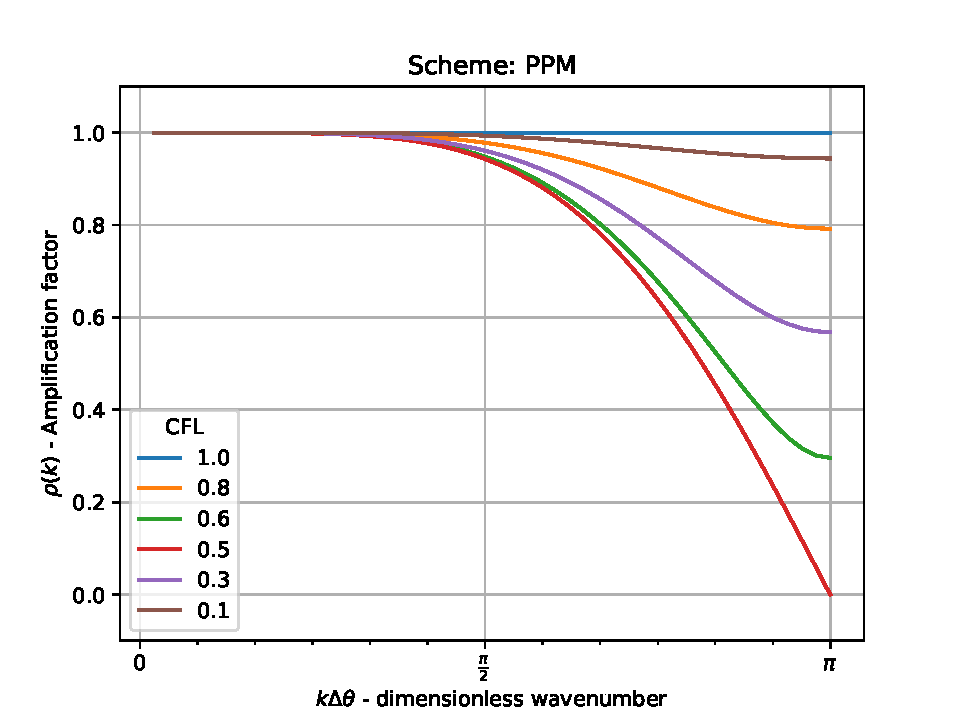
\includegraphics[width=0.49\linewidth]{stability_PPM}
	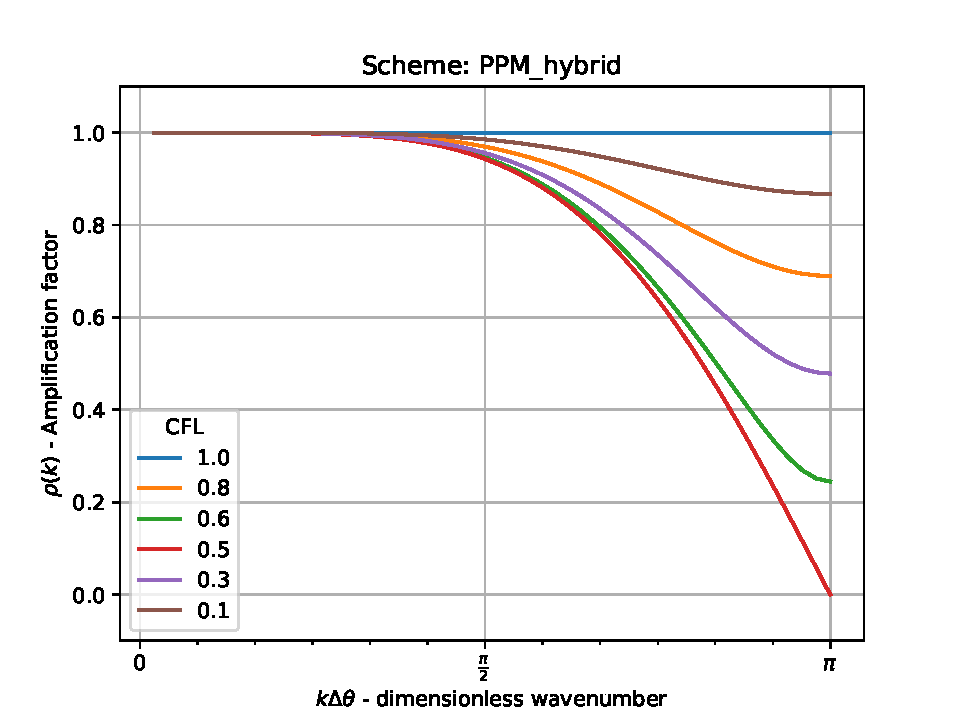
\includegraphics[width=0.49\linewidth]{stability_PPM_hybrid}
	\caption{Amplification factor for the PPM (left) and hybrid PPM (right) schemes for different CFL numbers.}
	\label{chp2-fig-amplification}
\end{figure}
In order to investigate the consistency of the PPM scheme, we notice that when we are deducing the time average flux, 
we are making approximations of the form:
\begin{equation}
	\label{chp2-sec-flux:analysis-eq1}
	\int_{t^n}^{t^{n+1}} (uq)(x_{i+\frac{1}{2}},t) \,dt \approx
	\int_{x_{i+\frac{1}{2}}-\tilde{u}_{i+\frac{1}{2}}^n \Delta t}^{x_{i+\frac{1}{2}}}
	q_{PP}(x;Q^n)\,dx, 
\end{equation}
as we can see from Equations \eqref{chp-sec-flux:fL_1} and \eqref{chp-sec-flux:fR_1},
which basically replace $q$ by $q_{PP}$ and $X(t^n, t^{n+1},x_{i+\frac{1}{2}})$ by 
$x_{i+\frac{1}{2}}-\tilde{u}_{i+\frac{1}{2}}^n \Delta t$
on the right-hand side of Equation \eqref{chp2-sec-flux:approx1}.
As we shall see, the approximation \eqref{chp2-sec-flux:analysis-eq1}
has two sources of error: one related to the departure point estimation and another due to the
parabolic approximation.
The next Proposition \eqref{chp2-sec-flux:prop2} investigates how the departure point error
impacts on the approximation \eqref{chp2-sec-flux:analysis-eq1} replacing $q_{PP}$ by $q$.

\begin{prop}
	\label{chp2-sec-flux:prop2}
	Assume the framework of Problem \ref{chp2-sec2-prob2} with $q \in \mathcal{C}^1$  and $u \in \mathcal{C}^P$, for some $P\geq2$. 
	Furthermore, assume the CFL condition and that $\Delta x$ and $ \Delta t $ are small enough as in Proposition \ref{chp2-sec-flux:departurebound}.
	
	Assume also that for some time-average velocity $\tilde{u}^n_{i+\frac{1}{2}}$, we have
	$X(t^n,t^{n+1};x_{i+\frac{1}{2}}) = x_{i+\frac{1}{2}} - \tilde{u}^n_{i+\frac{1}{2}}\Delta t + C_{i+\frac{1}{2}}\Delta t^P$, 
	where the constants $C_{i+\frac{1}{2}}$ can be written as $C_{i+\frac{1}{2}} = F(\tilde{x}_{i+\frac{1}{2}}, \tilde{t}_{i+\frac{1}{2}})$ for 
	a $\mathcal{C}^1$ function $F:[a,b]^d \times [0,T]^d \to \mathbb{R}$ . 
	Besides that, assume $\tilde{x}_{i+\frac{1}{2}} \in [x_{i+\frac{1}{2}}-k\Delta x, x_{i+\frac{1}{2}} + k\Delta x]^d$, 
	where $k$ do not depend on $\Delta x$ and $\tilde{t}_{i+\frac{1}{2}} \in [t^n, t^{n+1}]^d$.
	Under all these assumptions, we have:
\begin{align*}
	&\bigg|\int_{t^n}^{t^{n+1}} (uq)(x_{i+\frac{1}{2}},s) \,ds 
	-\int^{x_{i+\frac{1}{2}}}_{x_{i+\frac{1}{2}}-\tilde{u}_{i+\frac{1}{2}}^n \Delta t} q(x,t^n)\,dx
	-\bigg( \int_{t^n}^{t^{n+1}} (uq)(x_{i-\frac{1}{2}},s) \,ds 
	-\int^{x_{i-\frac{1}{2}}}_{x_{i-\frac{1}{2}}-\tilde{u}_{i-\frac{1}{2}}^n \Delta t} q(x,t^n)\,dx  \bigg) \bigg| \\
	& \leq K_1 \Delta t^{P+1},
\end{align*}
	where $K_1$ depends on $q$ and $u$.
\end{prop}
\begin{proof}
	Using Equation \eqref{chp2-sec-flux:approx1} and the mean value theorem for integrals, we get: 
	\begin{align*}
	\label{chp-sec-flux:depint_5}
			  &\int_{t^n}^{t^{n+1}} (uq)(x_{i+\frac{1}{2}},s) \,ds 
			 -\int^{x_{i+\frac{1}{2}}}_{x_{i+\frac{1}{2}}-\tilde{u}_{i+\frac{1}{2}}^n \Delta t} q(x,t^n)\,dx =
			 \int^{x_{i+\frac{1}{2}}}_{X(t^n,t^{n+1};x_{i+\frac{1}{2}})} q(x,t^n)\,dx
			 -\int^{x_{i+\frac{1}{2}}}_{x_{i+\frac{1}{2}}-\tilde{u}_{i+\frac{1}{2}}^n \Delta t} q(x,t^n)\,dx \\ 
			 &= \int_{X(t^n,t^{n+1};x_{i+\frac{1}{2}})}^{x_{i+\frac{1}{2}}-\tilde{u}_{i+\frac{1}{2}}^n \Delta t} q(x,t^n)\,dx  
			 = \big(X(t^n,t^{n+1};x_{i+\frac{1}{2}}) - x_{i+\frac{1}{2}}+\tilde{u}_{i+\frac{1}{2}}^n \Delta t \big)
			 q(\mu_i,t^n) =  F(\tilde{x}_{i+\frac{1}{2}}, \tilde{t}_{i+\frac{1}{2}}) \Delta t^P q(\mu_{i+\frac{1}{2}},t^n),
	\end{align*}
	for some $\mu_{i+\frac{1}{2}} \in X_{i}\cup X_{i+1}$. Similarly, we have:
	\begin{align*}
	&\int_{t^n}^{t^{n+1}} (uq)(x_{i-\frac{1}{2}},s) \,ds 
	-\int^{x_{i-\frac{1}{2}}}_{x_{i-\frac{1}{2}}-\tilde{u}_{i-\frac{1}{2}}^n \Delta t} q(x,t^n)\,dx =
	F(\tilde{x}_{i-\frac{1}{2}},\tilde{t}_{i-\frac{1}{2}}) \Delta t^P q(\mu_{i-\frac{1}{2}},t^n),
	\end{align*}
and again, $\mu_{i-\frac{1}{2}} \in X_{i-1}\cup X_{i}$
We introduce the following auxiliary $\mathcal{C}^1$ function:
\begin{equation*}
	G(\nu) = F(\nu_1,\nu_2)q(\nu_3,t^n).
\end{equation*}
where $\nu =(\nu_1,\nu_2, \nu_3)$, $\nu_1 \in [a,b]^d$, $\nu_2 \in [0, T]^d$, $\nu_3 \in [a,b]$.
Introducing $\nu_{i+\frac{1}{2}} = (\tilde{x}_{i+\frac{1}{2}}, \tilde{t}_{i+\frac{1}{2}}, \mu_{i+\frac{1}{2}})$,
$\nu_{i-\frac{1}{2}} = (\tilde{x}_{i-\frac{1}{2}}, \tilde{t}_{i-\frac{1}{2}}, \mu_{i-\frac{1}{2}})$
and using the mean value theorem, we have:
\begin{align*}
	|G(\nu_{i+\frac{1}{2}})-G(\nu_{i-\frac{1}{2}})|  
	&\leq \bigg(\sup_{\nu \in [a,b]^d\times[0,T]^d\times[a,b]}{\|\nabla G(\nu) \|_{2d+1}} \bigg)\|\nu_{i+\frac{1}{2}}-\nu_{i-\frac{1}{2}}\|_{2d+1} \\
	&\leq \bigg(\sqrt{(d(2k+1)^2 + 9){\lambda^2}+d}\sup_{\nu \in [a,b]^d\times[0,T]^d\times[a,b]}{\|\nabla G(\nu) \|_{2d+1}} \bigg) \Delta t,
\end{align*}
where $\|\cdot\|_{D}$ is the 2-norm of $\mathbb{R}^{D}$ and we used that $\|\tilde{x}_{i+\frac{1}{2}}-\tilde{x}_{i-\frac{1}{2}}\|_{d}^2  \leq d(2k+1)^2\Delta x^2$, 
$|\tilde{\mu}_{i+\frac{1}{2}}-\tilde{\mu}_{i-\frac{1}{2}}| \leq 3 \Delta x$,
and $\|\tilde{t}_{i+\frac{1}{2}}-\tilde{t}_{i-\frac{1}{2}}\|_{d}^2 \leq d\Delta t^2$.
Finally, we have the desired bound:
\begin{align*}
	&\bigg|\int_{t^n}^{t^{n+1}} (uq)(x_{i+\frac{1}{2}},s) \,ds 
	-\int^{x_{i+\frac{1}{2}}}_{x_{i+\frac{1}{2}}-\tilde{u}_{i+\frac{1}{2}}^n \Delta t} q(x,t^n)\,dx
	-\bigg( \int_{t^n}^{t^{n+1}} (uq)(x_{i-\frac{1}{2}},s) \,ds 
	-\int^{x_{i-\frac{1}{2}}}_{x_{i-\frac{1}{2}}-\tilde{u}_{i-\frac{1}{2}}^n \Delta t} q(x,t^n)\,dx  \bigg) \bigg| \\
	&=|(G(\nu_{i+\frac{1}{2}})-G(\nu_{i-\frac{1}{2}}))|\Delta t^P \leq  K_1 \Delta t^{P+1},
\end{align*}
where $K_1 = \sqrt{(d(2k+1)^2 + 9){\lambda^2}+d}\sup_{\nu \in [a,b]^d\times[0,T]^d\times[a,b]}{\|\nabla G(\nu) \|_{2d+1}}$.
\end{proof}
\begin{remark}
If the departure point is computed using Equation \eqref{chp-sec-flux:departurepoint3}, it follows from Proposition \ref{chp-sec-flux:dp_euler}
that $P=2$, $k=3$, $d=2$.
The function $F$ is defined by the right-hand side of Equation \eqref{chp-sec-flux:departurepoint6}.
\end{remark}
The next proposition gives a measure of the impact of the Piecewise-Parabolic approximation
on the time average flux, considering this last computed using an estimated departure point.
\begin{prop}
	\label{chp2-sec-flux:prop3}
	Assume the framework of Problem \ref{chp2-sec2-prob2}.
	If $q \in \mathcal{C}^5$ and $u \in \mathcal{C}^1$, then:
	\begin{align*}
	 &\bigg|
	\frac{1}{\Delta t}\int^{x_{i+\frac{1}{2}}}_{x_{i+\frac{1}{2}}-\tilde{u}_{i+\frac{1}{2}}^n \Delta t} q(x,t^n)\,dx -
	\mathcal{F}(Q(t_n)(\mathcal{S}_{i+\frac{1}{2}}),\tilde{u}^n_{i+\frac{1}{2}}) 
	-\bigg(\frac{1}{\Delta t}\int^{x_{i-\frac{1}{2}}}_{x_{i-\frac{1}{2}}-\tilde{u}_{i-\frac{1}{2}}^n \Delta t} q(x,t^n)\,dx -
	\mathcal{F}(Q(t_n)\mathcal{S}_{i-\frac{1}{2}},\tilde{u}^n_{i-\frac{1}{2}})\bigg) \bigg|\\
	&\leq K_2\Delta x^4,
	\end{align*}
	where $K_2$ depends on $q$ and $u$.
\end{prop}
\begin{proof}
	We denote by $q_{PP}$ the piecewise-parabolic approximation of $Q(t^n)$. Then:
	\begin{equation*}
	\frac{1}{\Delta t}\int^{x_{i+\frac{1}{2}}}_{x_{i+\frac{1}{2}}-\tilde{u}_{i+\frac{1}{2}}^n \Delta t} q(x,t^n)\,dx -
	\mathcal{F}(Q(t_n)(\mathcal{S}_{i+\frac{1}{2}}),\tilde{u}^n_{i+\frac{1}{2}}) = 	
	\frac{1}{\Delta t}\int^{x_{i+\frac{1}{2}}}_{x_{i+\frac{1}{2}}-\tilde{u}_{i+\frac{1}{2}}^n \Delta t} q(x,t^n)\,dx -
	\frac{1}{\Delta t}\int^{x_{i+\frac{1}{2}}}_{x_{i+\frac{1}{2}}-\tilde{u}_{i+\frac{1}{2}}^n \Delta t} q_{PP}(x;Q(t^n))\,dx
	\end{equation*}
	and
	\begin{equation*}
	\frac{1}{\Delta t}\int^{x_{i-\frac{1}{2}}}_{x_{i-\frac{1}{2}}-\tilde{u}_{i-\frac{1}{2}}^n \Delta t} q(x,t^n)\,dx -
	\mathcal{F}(Q(t_n)(\mathcal{S}_{i-\frac{1}{2}}),\tilde{u}^n_{i-\frac{1}{2}}) = 	
	\frac{1}{\Delta t}\int^{x_{i-\frac{1}{2}}}_{x_{i-\frac{1}{2}}-\tilde{u}_{i-\frac{1}{2}}^n \Delta t} q(x,t^n)\,dx -
	\frac{1}{\Delta t}\int^{x_{i-\frac{1}{2}}}_{x_{i-\frac{1}{2}}-\tilde{u}_{i-\frac{1}{2}}^n \Delta t} q_{PP}(x;Q(t^n))\,dx.
\end{equation*}
	Similarly to Proposition \ref{prop:ppm-bound4}, we can write:
	\begin{align*}
		q(x,t^n)-q_{PP}(x;Q(t^n)) = &C_1(\mu_1, \mu_2) \Delta x ^4 + C_2(\mu_3, \mu_4) \Delta x ^2(x-x_L)
		+ \frac{C_3}{2}(\mu_5, \mu_6)\Delta x (x-x_L)^2  \\&+C_4(\mu_7)(x-x_L)^3,
	\end{align*}
	where $C_1, C_2$, $C_3$ and $C_4$ are given by Equations \eqref{prop:ppm-bound1-eq3},
	\eqref{prop:ppm-bound2-eq2}, \eqref{prop:ppm-bound3-eq2} and \eqref{prop:ppm-bound4-eq3} respectively,
	$x_L$ is the left boundary of the control volume that contains $x$ ($X_i$ or $X_{i+1}$) and 
	$\mu_k \in [x_{i+\frac{1}{2}} - 3\Delta x,x_{i+\frac{1}{2}} + 3\Delta x]$, $\forall k =1, \cdots, 7$.
	Similarly to Proposition \ref{chp2-sec-flux:prop2}, using the mean value theorem for integrals, one can write:
	\begin{equation}
	\label{chp2-sec-flux:prop3-eq1}
	\int^{x_{i+\frac{1}{2}}}_{x_{i+\frac{1}{2}}-\tilde{u}_{i+\frac{1}{2}}^n \Delta t} (q(x,t^n)-q_{PP}(x;Q(t^n)))\,dx
	= F(\mu^1)\Delta x^4,
	\end{equation}
	and
	\begin{equation}
	\label{chp2-sec-flux:prop3-eq2}
	\int^{x_{i-\frac{1}{2}}}_{x_{i-\frac{1}{2}}-\tilde{u}_{i-\frac{1}{2}}^n \Delta t} (q(x,t^n)-q_{PP}(x;Q(t^n)))\,dx
	= F(\mu^2)\Delta x^4,
	\end{equation}
	for an auxiliary function $F:[a,b]^8 \to \mathbb{R}$, $F\in\mathcal{C}^1$, where $F$ depends on $q$, $u$,
	and $C_1, C_2, C_3$ and $C_4$. Subtracting Equation \eqref{chp2-sec-flux:prop3-eq2} from Equation \eqref{chp2-sec-flux:prop3-eq1}
	and using the mean value theorem, we get the desired inequality.
	\end{proof}
Now we are able to tackle the consistency problem on the next proposition.
\begin{prop}
	Assume the same hypothesis of Proposition \ref{chp2-sec-flux:prop2} and Proposition \ref{chp2-sec-flux:prop3}.
	Denote by $q_{PP}$ the Piecewise-Parabolic approximation of $q(x,t^n)$. Then, the LTE given by Equation
	\eqref{consistency-1d-eq2} satisfies:
	\begin{equation}
		|\tau_i^n|\leq M_1 \Delta t^{P-1} + M_2\Delta x^3,
	\end{equation}
	where $M_1$ and $M_2$ are constants depending only on $q$ and $u$.
\end{prop}
\begin{proof}
	We have:
	\begin{align*}
	 &\Delta x  \tau_i^n = \bigg|
	 \frac{1}{\Delta t}\int_{t^n}^{t^{n+1}} (uq)(x_{i+\frac{1}{2}},s) \,ds - 
	 \mathcal{F}(Q(t_n)(\mathcal{S}_{i+\frac{1}{2}}),\tilde{u}^n_{i+\frac{1}{2}})
	 - \frac{1}{\Delta t}\int_{t^n}^{t^{n+1}} (uq)(x_{i-\frac{1}{2}},s) \,ds +
	 \mathcal{F}(Q(t_n)(\mathcal{S}_{i-\frac{1}{2}}),\tilde{u}^n_{i-\frac{1}{2}}) \bigg| = \\
	 & \frac{1}{\Delta t} \bigg|
	 \int_{t^n}^{t^{n+1}} (uq)(x_{i+\frac{1}{2}},s) \,ds - 
	 \int^{x_{i+\frac{1}{2}}}_{x_{i+\frac{1}{2}}-\tilde{u}_{i+\frac{1}{2}}^n \Delta t} q_{PP}(x)\,dx
	 -\bigg(\int_{t^n}^{t^{n+1}} (uq)(x_{i-\frac{1}{2}},s) \,ds - 
	 \int^{x_{i-\frac{1}{2}}}_{x_{i-\frac{1}{2}}-\tilde{u}_{i-\frac{1}{2}}^n \Delta t} q_{PP}(x)\,dx  
	  \bigg)\bigg| =\\
	 &\frac{1}{\Delta t} \bigg|
	 \int_{t^n}^{t^{n+1}} (uq)(x_{i+\frac{1}{2}},s) \,ds 
	-\int^{x_{i+\frac{1}{2}}}_{x_{i+\frac{1}{2}}-\tilde{u}_{i+\frac{1}{2}}^n \Delta t} q(x,t^n)\,dx 
	+\int^{x_{i+\frac{1}{2}}}_{x_{i+\frac{1}{2}}-\tilde{u}_{i+\frac{1}{2}}^n \Delta t} q(x,t^n)\,dx 
	-\int^{x_{i+\frac{1}{2}}}_{x_{i+\frac{1}{2}}-\tilde{u}_{i+\frac{1}{2}}^n \Delta t} q_{PP}(x)\,dx \\
	 &-\bigg(\int_{t^n}^{t^{n+1}} (uq)(x_{i-\frac{1}{2}},s) \,ds 
	-\int^{x_{i-\frac{1}{2}}}_{x_{i-\frac{1}{2}}-\tilde{u}_{i-\frac{1}{2}}^n \Delta t} q(x,t^n)\,dx 
	+\int^{x_{i-\frac{1}{2}}}_{x_{i-\frac{1}{2}}-\tilde{u}_{i-\frac{1}{2}}^n \Delta t} q(x,t^n)\,dx 
	-\int^{x_{i-\frac{1}{2}}}_{x_{i-\frac{1}{2}}-\tilde{u}_{i-\frac{1}{2}}^n \Delta t} q_{PP}(x)\,dx 
	 \bigg) \bigg| \leq \\
	 &\frac{1}{\Delta t} \bigg|
	\int_{t^n}^{t^{n+1}} (uq)(x_{i+\frac{1}{2}},s) \,ds 
	-\int^{x_{i+\frac{1}{2}}}_{x_{i+\frac{1}{2}}-\tilde{u}_{i+\frac{1}{2}}^n \Delta t} q(x,t^n)\,dx 
	-\bigg(\int_{t^n}^{t^{n+1}} (uq)(x_{i-\frac{1}{2}},s) \,ds 
	-\int^{x_{i-\frac{1}{2}}}_{x_{i-\frac{1}{2}}-\tilde{u}_{i-\frac{1}{2}}^n \Delta t} q(x,t^n)\,dx \bigg)\bigg|+\\
     &\frac{1}{\Delta t}\bigg| 
	 \int^{x_{i+\frac{1}{2}}}_{x_{i+\frac{1}{2}}-\tilde{u}_{i+\frac{1}{2}}^n \Delta t} q(x,t^n)\,dx 
	-\int^{x_{i+\frac{1}{2}}}_{x_{i+\frac{1}{2}}-\tilde{u}_{i+\frac{1}{2}}^n \Delta t} q_{PP}(x) \,dx 
	-\bigg(\int^{x_{i-\frac{1}{2}}}_{x_{i-\frac{1}{2}}-\tilde{u}_{i-\frac{1}{2}}^n \Delta t} q(x,t^n)\,dx 
	-\int^{x_{i-\frac{1}{2}}}_{x_{i-\frac{1}{2}}-\tilde{u}_{i-\frac{1}{2}}^n \Delta t} q_{PP}(x) \,dx 
	\bigg) \bigg| 
	\end{align*}
	Therefore, it follows from Propositions \ref{chp2-sec-flux:prop2} and \ref{chp2-sec-flux:prop3} that
	\begin{align*}
		|\tau_i^n| \leq \frac{1}{\Delta x \Delta t} K_1 \Delta t^{P+1} + \frac{1}{\Delta x} K_2 \Delta x^4 = 
		K_1 \lambda \Delta t^{P-1} + K_2 \Delta x^3,
	\end{align*}
	from which the proposition follows.
\end{proof}

	Thus, it follows from Proposition \ref{chp2-sec-flux:prop3} that the PPM scheme is consistent in the $\infty$-norm
	and has two sources of error: one related to the departure point calculation and another due to the parabolic approximation.
	In particular, the PPM flux using the departure point from Equation \eqref{chp-sec-flux:departurepoint3}, 
	we have a first-order error related to the departure point computation. 
	We point out that, if the velocity is constant, then no error is obtained
	using the PPM flux, except for the approximation $q_{PP}$ to $q$.
\newpage
\section{Numerical experiments}
\label{chp2-sec-numerical-exp}
This Section is dedicated to presenting the numerical results of the PPM and its variations discussed here.
For non-monotonic schemes, we are going to consider
the original PPM from \citet{colella:1984} and the hybrid PPM from \citet{putman:2007}.
For monotonic schemes, we are going to consider the monotonization schemes from 
\citet{colella:1984} and \citet{lin:2004}, which are referred to as CW84 monotonization 
and L04 monotonization hereafter.
In Subsection \ref{chp2-sec-numerical-exp-1} we present results 
using the linear advection equation with constant velocity
and in Subsection \ref{chp2-sec-numerical-exp-2}
the results are based on the linear advection equation with variable velocity.
The code used in this Section may be found in Appendix \ref{anexo-code}.

\subsection{Linear advection equation with constant velocity simulations}
\label{chp2-sec-numerical-exp-1}
For the linear advection equation with the constant velocity we shall adopt the $u=0.2$ and 
a CFL number equal to $0.8$.
The spatial domain will be given by $[0,1]$ and the time integration interval will be $[0,5]$.
Since we are going to assume periodic boundary conditions, the period is equal to $5$. 
Hence, the simulations presented here shall advect an initial profile for one time period. 
This shall be the general setup for all simulations presented in this subsection. 
What will distinguish the simulations is the initial condition.
The first $q_0$ is given by:
\begin{equation}
	\label{chp2-ic1}
	q_0(x) = \sin (2\pi k x) + 1.
\end{equation}
Here $k$ denotes the wavenumber and we adopt $k=5$.
Inspired by \citet{trefethen:2000}, we adopted the following periodic Gaussian profile.
\begin{equation}
	\label{chp2-ic2}
		q_0(x) = \exp(-10\cos^2 (2\pi x)).
\end{equation}
Both functions from Equations \eqref{chp2-ic2} and \eqref{chp2-ic2} are smooth.
We also consider a discontinuous initial condition given by:
\begin{equation}
	\label{chp2-ic3}
		q_0(x) =  
  \begin{cases}
		1 & \text{if } x \in [0.4,0.6],\\
		0 & \text{otherwise}.
  \end{cases}
\end{equation}
It is easy to check that the  exact solution of Problem \ref{chp2-sec2-prob1}
is given by $q_0(x-ut)$ for all $q_0$ presented here.

As pointed in Subsection \ref{chp2-sub-CC}, when $q_0$ is given by Equation \eqref{chp2-ic2},
we are going to compute the initial average values $Q_i(0)$ using
the initial values of $q^0_i$ at the control volume centroids, which is second-order 
accurate by Proposition \ref{prop-bound-centroid}.
In the error calculation, only when $q_0$ is given by Equation \eqref{chp2-ic2},
we replace $Q_{i}(t^n)$ by its centroid value $q_{i}(t^n)$, which again gives
a second-order approximation by Proposition \ref{prop-bound-centroid}.
Therefore, since $q_0$ is smooth, we expect that the error convergence shall be at least second-order accurate.
Finally, the error norm is normalized by dividing the error norm by the exact solution norm. 
The norm adopted here is the maximum norm.

\newpage
\begin{figure}[!htb]
  \centering
  \begin{subfigure}{0.45\textwidth}
    \centering
			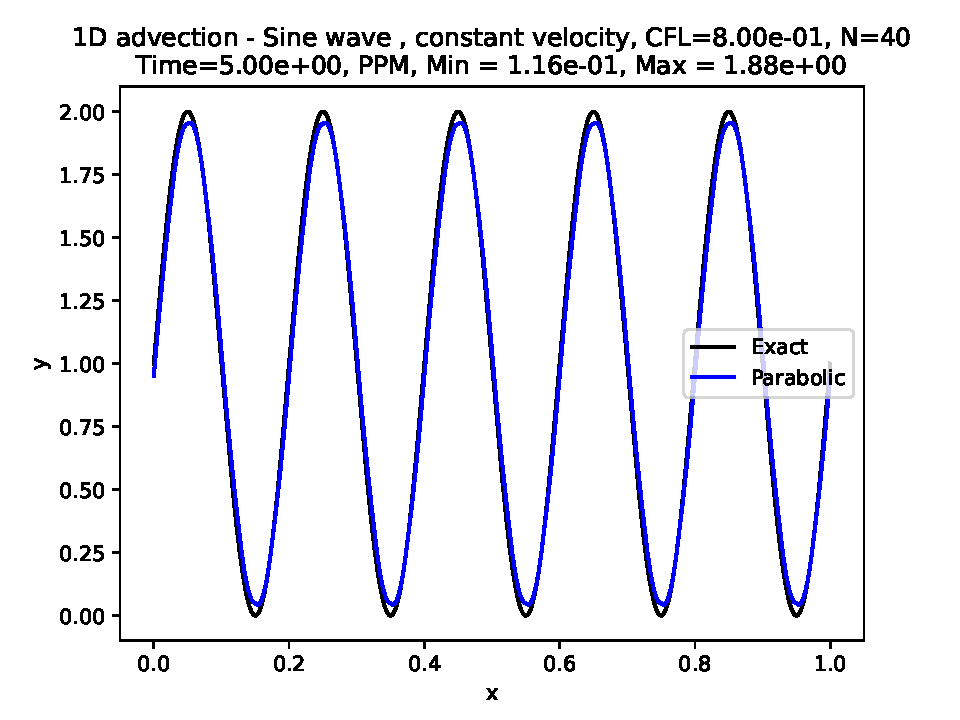
\includegraphics[width=1\linewidth]{1d_adv_tc2_ic1_vf1_t49_N40_PPM}
			\caption{PPM.\label{chp2-sec-exp-adv1-a}}
  \end{subfigure}
  \begin{subfigure}{0.45\textwidth}
    \centering
			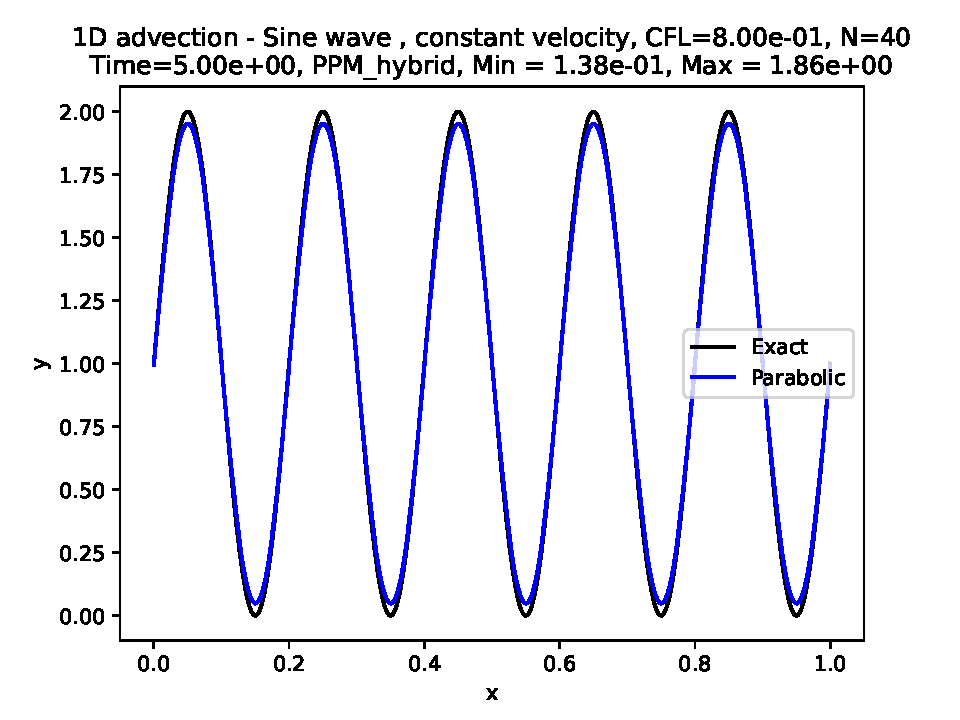
\includegraphics[width=1\linewidth]{1d_adv_tc2_ic1_vf1_t49_N40_PPM_hybrid}
			\caption{Hybrid PPM.\label{chp2-sec-exp-adv1-b}}
  \end{subfigure}

  \begin{subfigure}{0.45\textwidth}
    \centering
		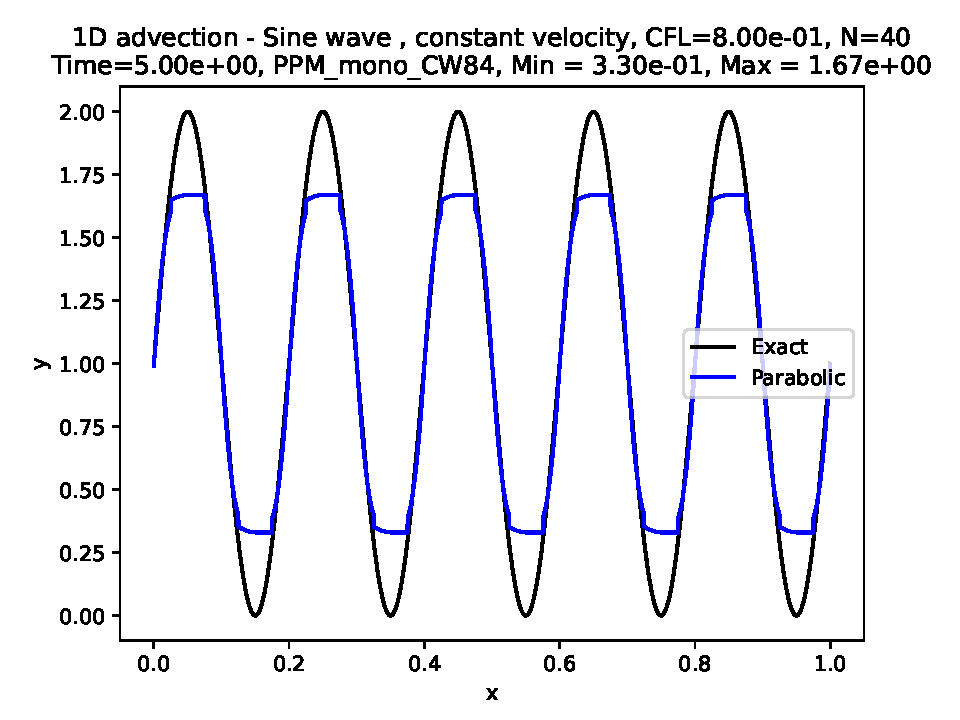
\includegraphics[width=1\linewidth]{1d_adv_tc2_ic1_vf1_t49_N40_PPM_mono_CW84}
    \caption{PPM + CW84 monotonization.\label{chp2-sec-exp-adv1-c}}
  \end{subfigure}
  \begin{subfigure}{0.45\textwidth}
    \centering
			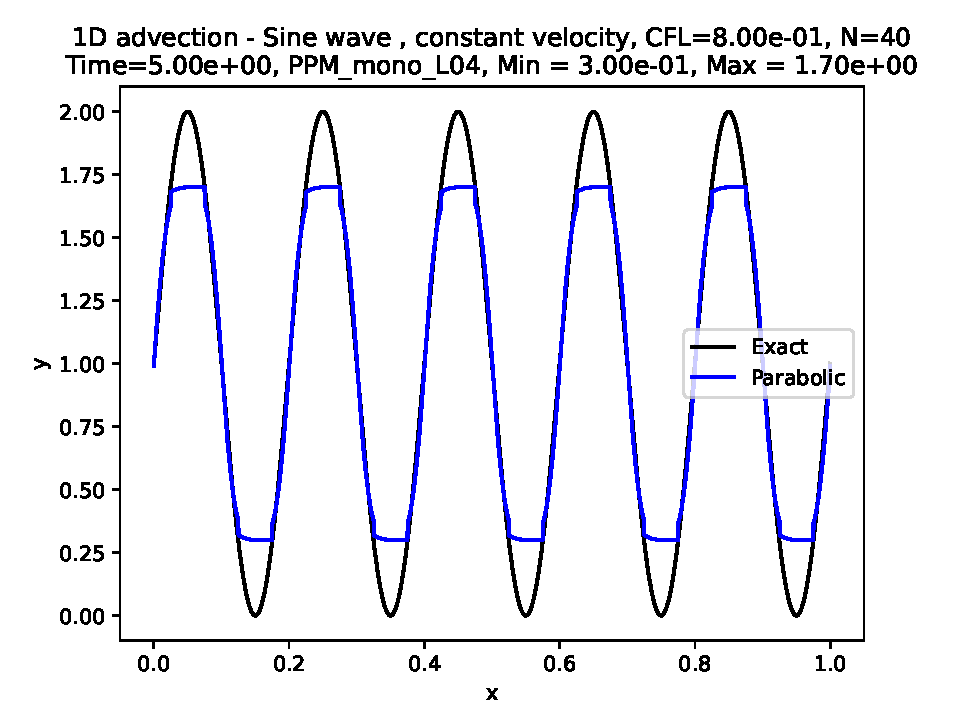
\includegraphics[width=1\linewidth]{1d_adv_tc2_ic1_vf1_t49_N40_PPM_mono_L04}
      \caption{PPM + L04 monotonization.\label{chp2-sec-exp-adv1-d}}
  \end{subfigure} 
	\caption{Linear advection experiment using a constant velocity equal to $0.1$,
  a CFL number equal to $0.8$, $N=40$ cells, and the initial condition is given by Equation \eqref{chp2-ic1}.
	These figures show the advected profile after 5 time units (one time period).
	Schemes employed: PPM (a), hybrid PPM (b), PPM with the CW84 monotonization
	(c) and PPM with L04 monotonization (d). \label{chp2-sec-exp-adv1}}
\end{figure}

\begin{figure}[!htb]
  \centering
  \begin{subfigure}{0.45\textwidth}
    \centering
		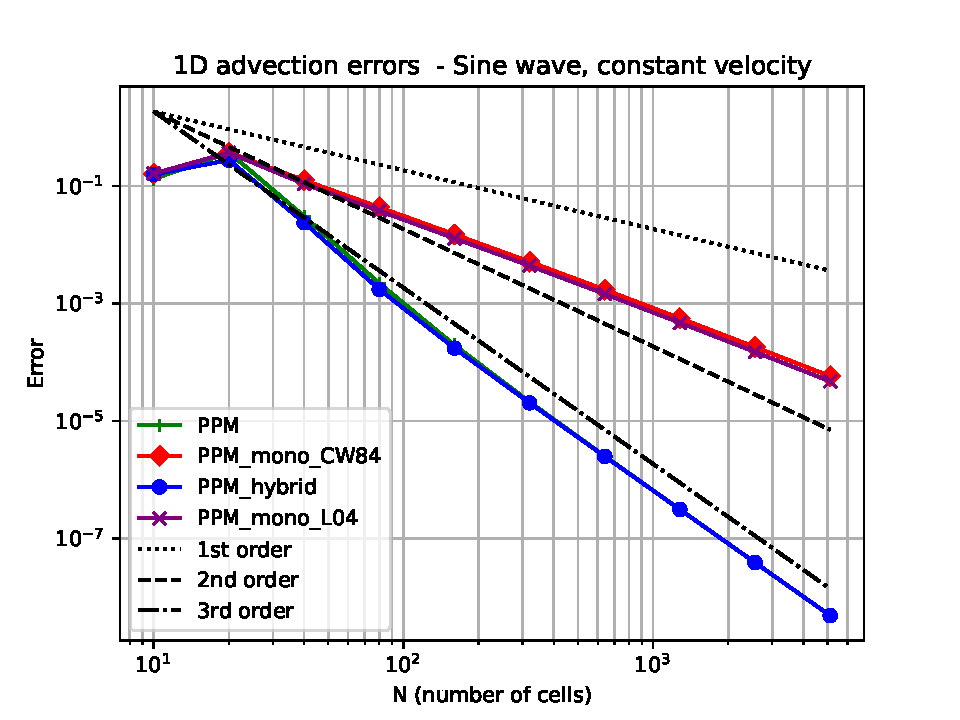
\includegraphics[width=1\linewidth]{1d_adv_tc2_ic1_vf1_parabola_errors}
		\caption{Error.\label{chp2-sec-exp-adv1-error}}
  \end{subfigure}
  \begin{subfigure}{0.45\textwidth}
    \centering
			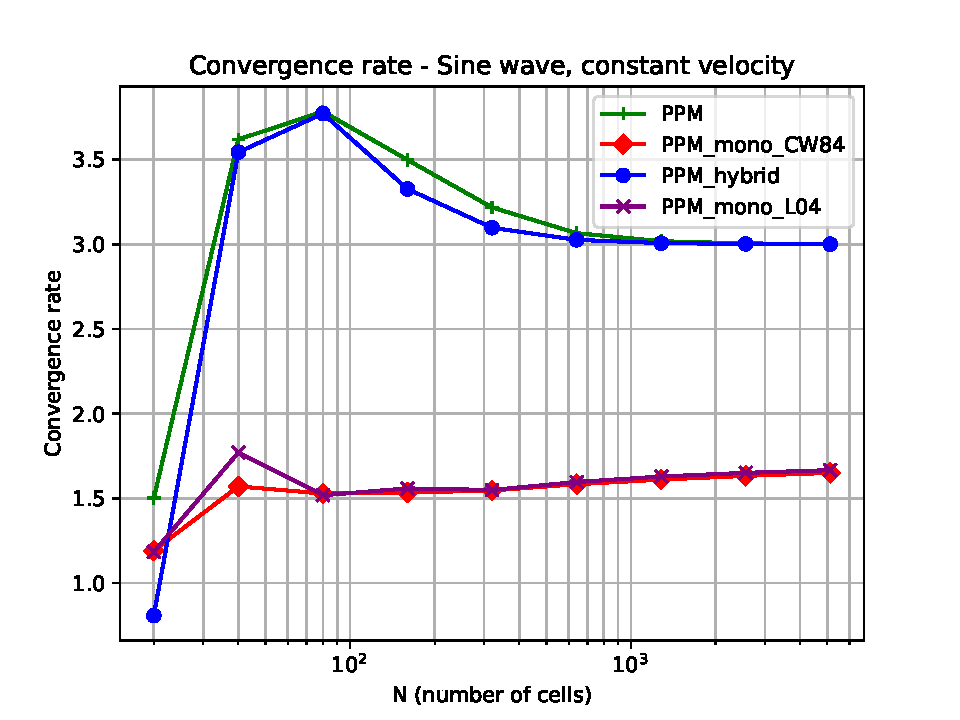
\includegraphics[width=1\linewidth]{1d_adv_tc2_ic1_vf1_convergence_rate}
		\caption{Convergence rate.\label{chp2-sec-exp-adv1-CR}}
  \end{subfigure}
	\caption{Convergence of the error (a) and convergence rate (b) for the schemes
  PPM, hybrid PPM, PPM with the CW84 monotonization and PPM with L04 monotonization
	applied to the linear advection problem using a constant velocity equal to $0.1$,
	a CFL number equal to $0.8$, a final time of integration equal to 5 time units
	and the initial condition given by Equation \eqref{chp2-ic1}.\label{chp2-sec-exp-adv1-2}}
\end{figure}

\newpage

\begin{figure}[!htb]
  \centering
  \begin{subfigure}{0.49\textwidth}
    \centering
			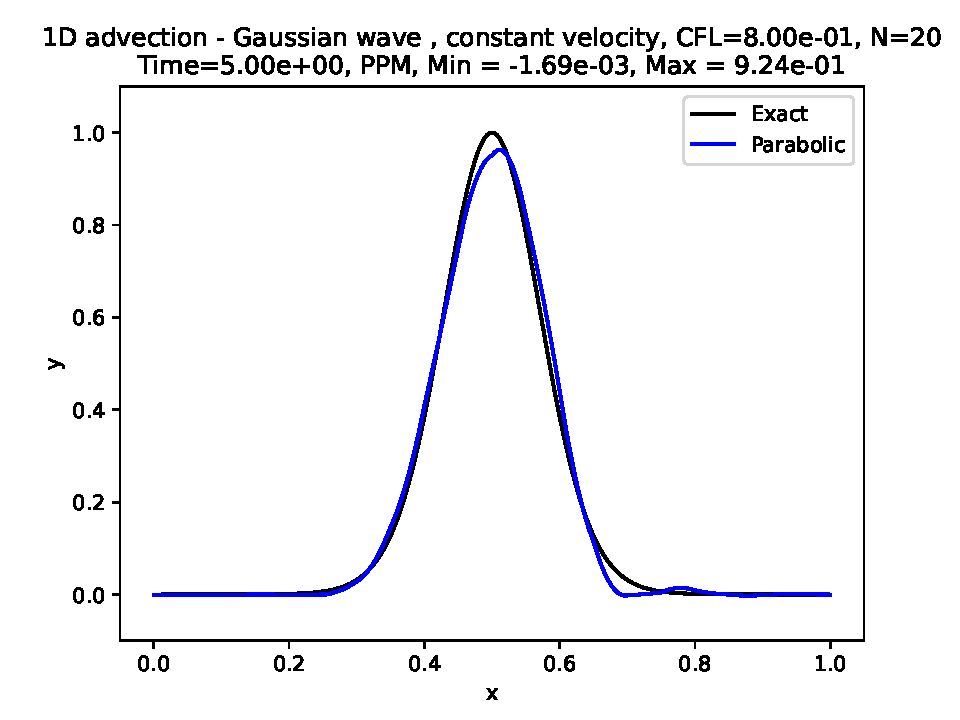
\includegraphics[width=1\linewidth]{1d_adv_tc2_ic2_vf1_t24_N20_PPM}
			\caption{PPM.\label{chp2-sec-exp-adv2-a}}
  \end{subfigure}
  \begin{subfigure}{0.49\textwidth}
    \centering
			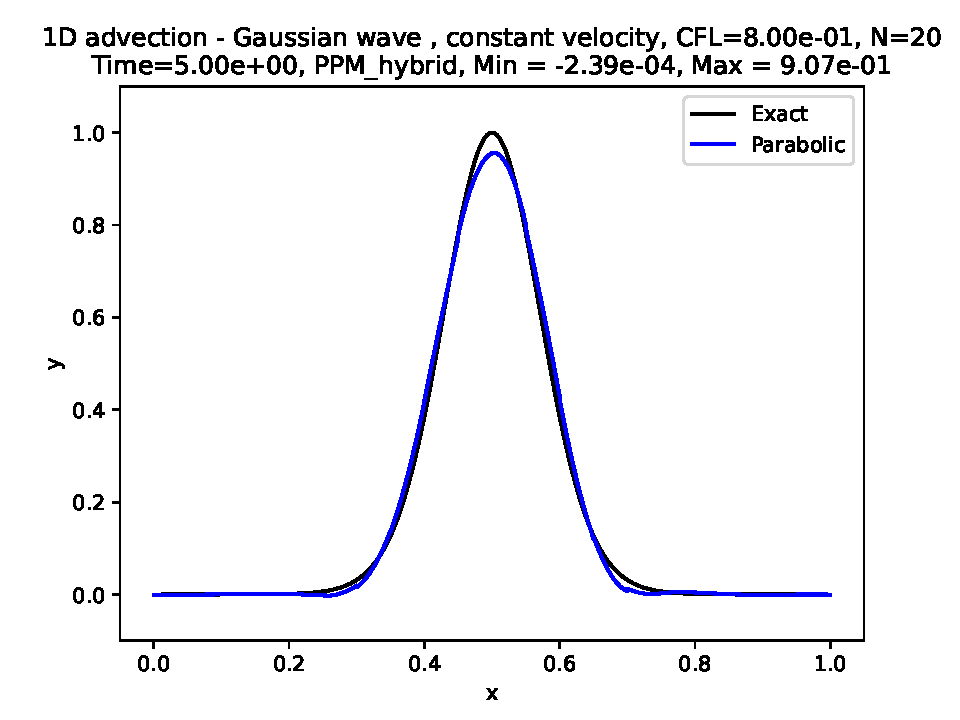
\includegraphics[width=1\linewidth]{1d_adv_tc2_ic2_vf1_t24_N20_PPM_hybrid}
			\caption{Hybrid PPM.\label{chp2-sec-exp-adv2-b}}
  \end{subfigure}

  \begin{subfigure}{0.49\textwidth}
    \centering
		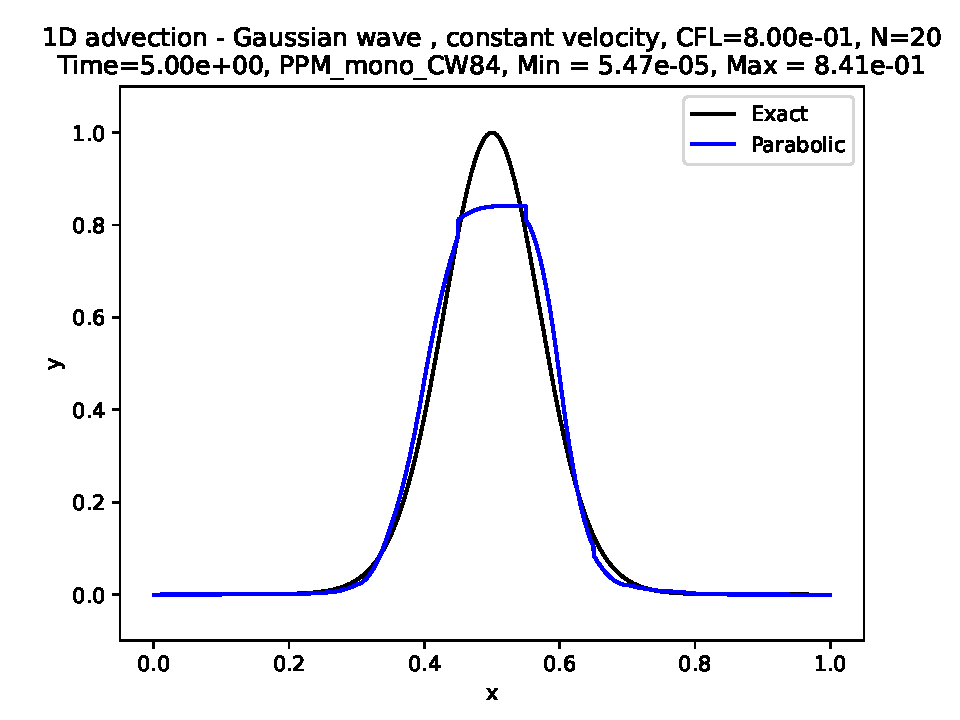
\includegraphics[width=1\linewidth]{1d_adv_tc2_ic2_vf1_t24_N20_PPM_mono_CW84}
    \caption{PPM + CW84 monotonization.\label{chp2-sec-exp-adv2-c}}
  \end{subfigure}
  \begin{subfigure}{0.49\textwidth}
    \centering
			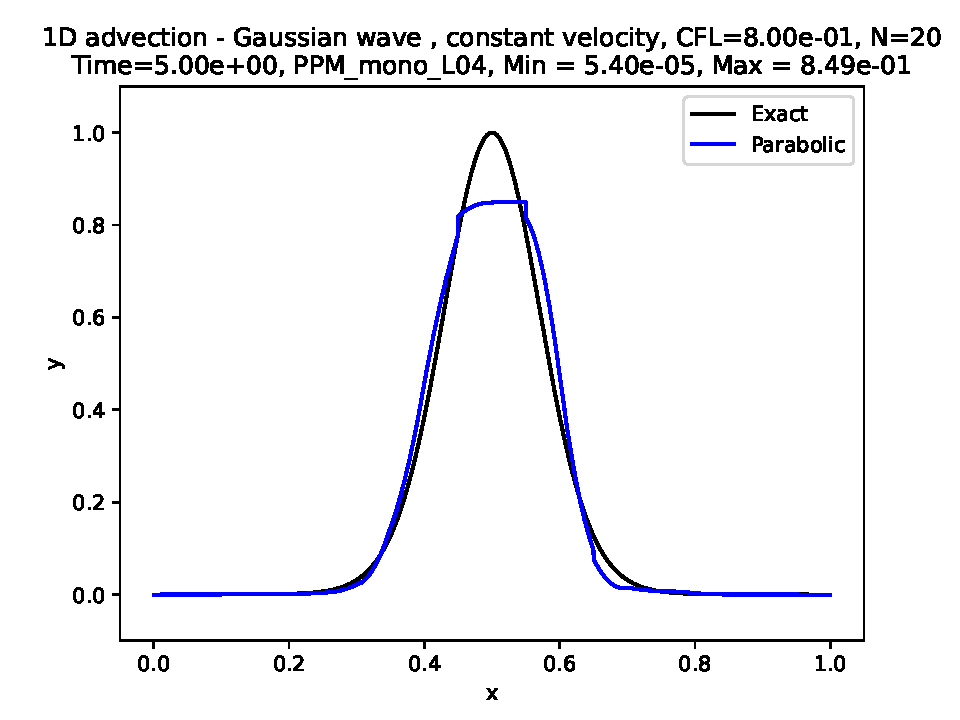
\includegraphics[width=1\linewidth]{1d_adv_tc2_ic2_vf1_t24_N20_PPM_mono_L04}
      \caption{PPM + L04 monotonization.\label{chp2-sec-exp-adv2-d}}
  \end{subfigure} 
	\caption{ Similar to Figure \ref{chp2-sec-exp-adv1} but using $N=20$
	and the initial condition given by Equation \eqref{chp2-ic2}.\label{chp2-sec-exp-adv2}}
\end{figure}

\begin{figure}[!htb]
  \centering
  \begin{subfigure}{0.49\textwidth}
    \centering
		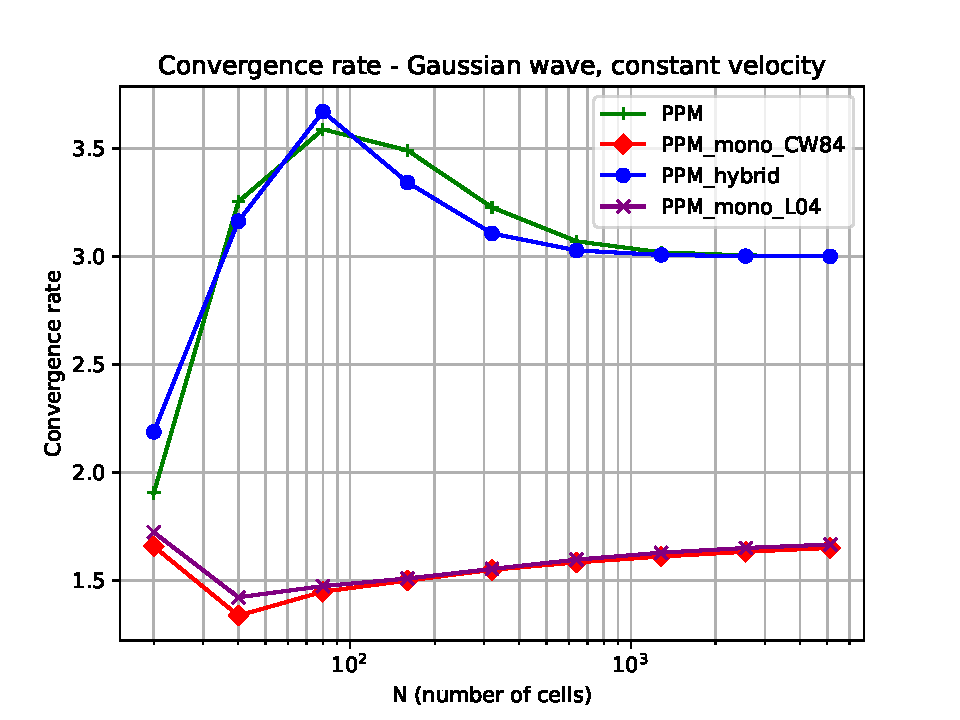
\includegraphics[width=1\linewidth]{1d_adv_tc2_ic2_vf1_convergence_rate}
		\caption{Error.\label{chp2-sec-exp-adv2-error}}
  \end{subfigure}
  \begin{subfigure}{0.49\textwidth}
    \centering
			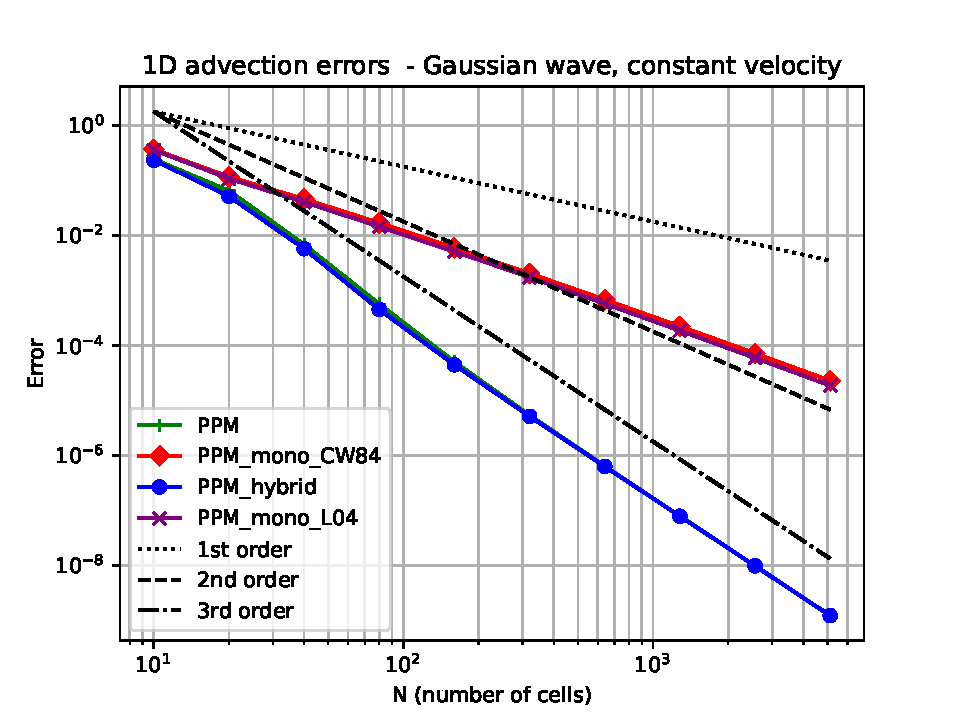
\includegraphics[width=1\linewidth]{1d_adv_tc2_ic2_vf1_parabola_errors}
		\caption{Convergence rate.\label{chp2-sec-exp-adv2-CR}}
  \end{subfigure}
	\caption{ Similar to Figure \ref{chp2-sec-exp-adv1-2} but using
	the initial condition given by Equation \eqref{chp2-ic2}. \label{chp2-sec-exp-adv2-2}}
\end{figure}

\newpage

\begin{figure}[!htb]
  \centering
  \begin{subfigure}{0.49\textwidth}
    \centering
			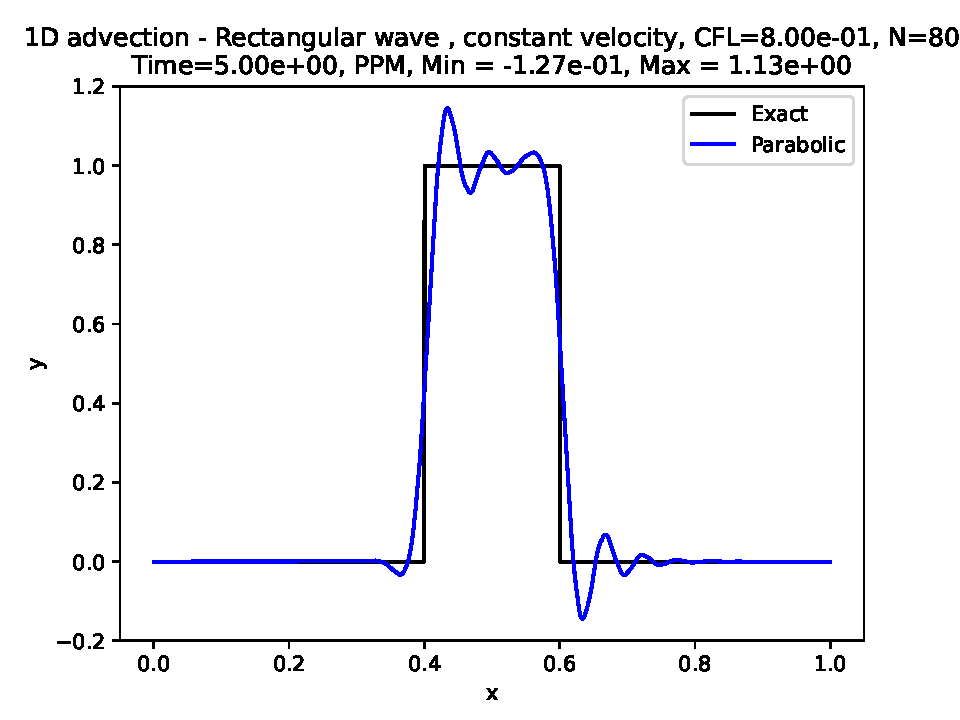
\includegraphics[width=1\linewidth]{1d_adv_tc2_ic4_vf1_t99_N80_PPM}
			\caption{PPM.\label{chp2-sec-exp-adv3-a}}
  \end{subfigure}
  \begin{subfigure}{0.49\textwidth}
    \centering
			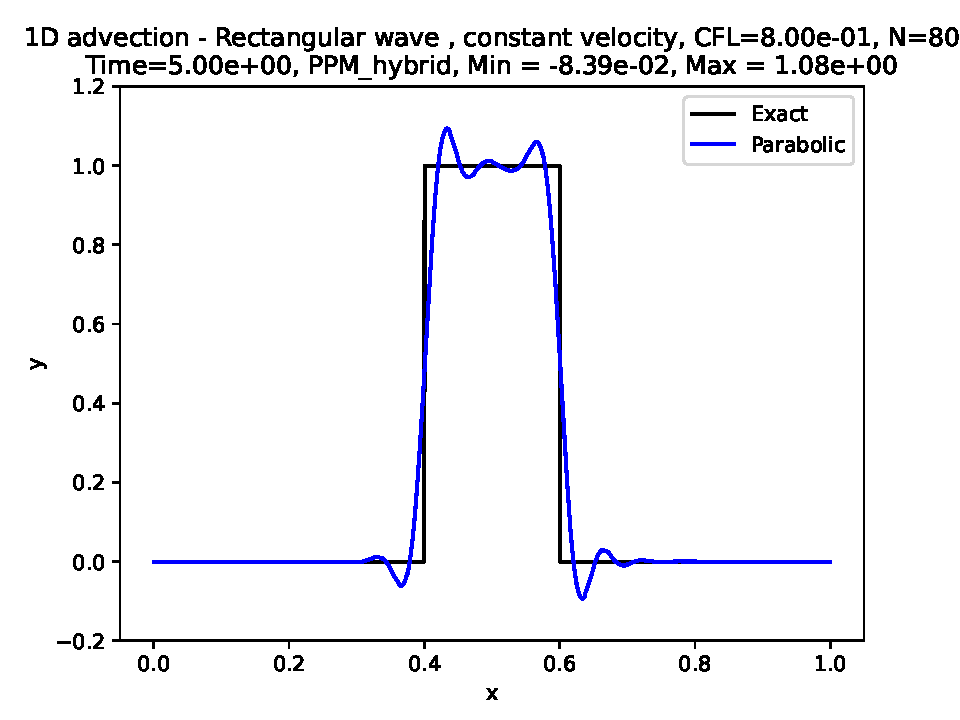
\includegraphics[width=1\linewidth]{1d_adv_tc2_ic4_vf1_t99_N80_PPM_hybrid}
			\caption{Hybrid PPM.\label{chp2-sec-exp-adv3-b}}
  \end{subfigure}

  \begin{subfigure}{0.49\textwidth}
    \centering
		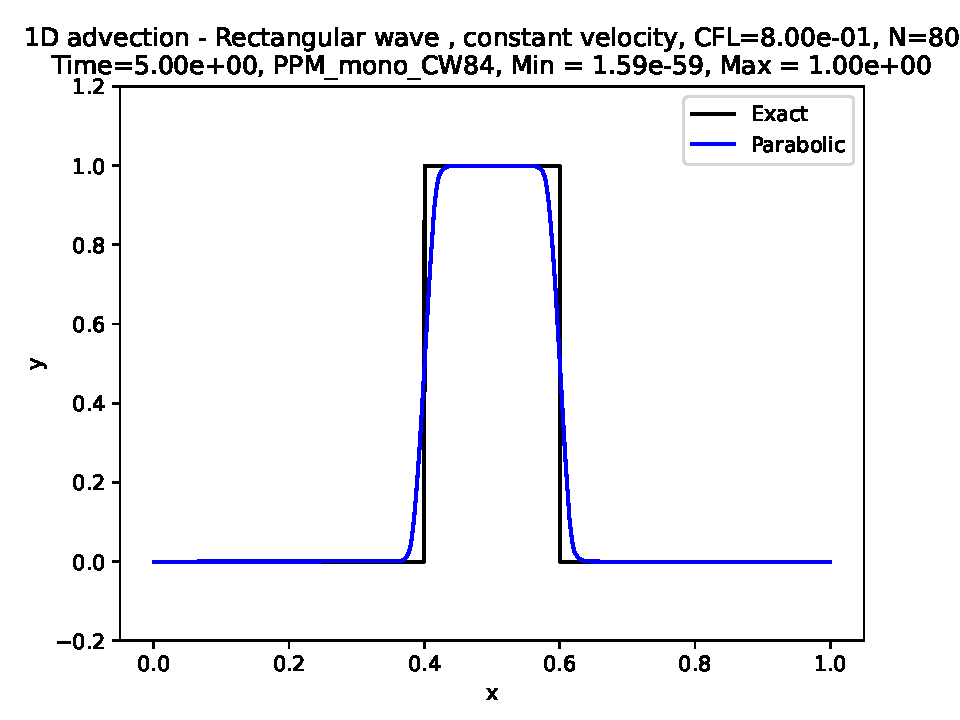
\includegraphics[width=1\linewidth]{1d_adv_tc2_ic4_vf1_t99_N80_PPM_mono_CW84}
    \caption{PPM + CW84 monotonization.\label{chp2-sec-exp-adv3-c}}
  \end{subfigure}
  \begin{subfigure}{0.49\textwidth}
    \centering
			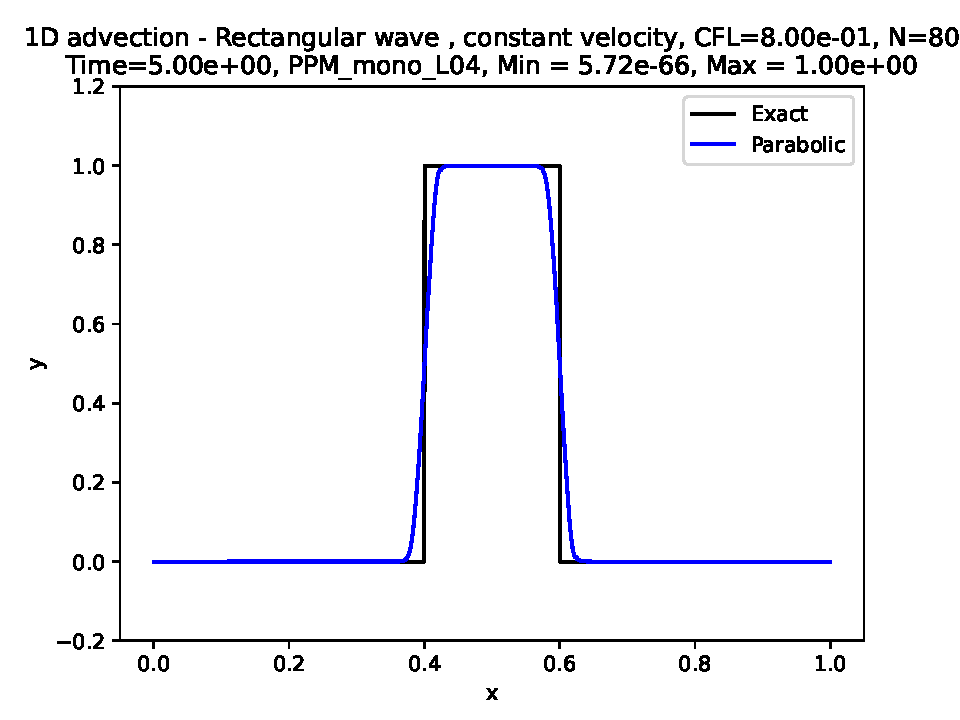
\includegraphics[width=1\linewidth]{1d_adv_tc2_ic4_vf1_t99_N80_PPM_mono_L04}
      \caption{PPM + L04 monotonization.\label{chp2-sec-exp-adv3-d}}
  \end{subfigure} 
	\caption{ Similar to Figure \ref{chp2-sec-exp-adv1} but using $N=80$
	and the initial condition given by Equation \eqref{chp2-ic3}.\label{chp2-sec-exp-adv3}}
\end{figure}
OKOK

\newpage

\subsection{Linear advection equation with variable velocity simulations}
\label{chp2-sec-numerical-exp-2}
In this Subsection, we shall investigate the how the PPM schemes behaves when the velocity is variable.
The initial condition is given by Equation \eqref{chp2-ic2}.
The relative errors are computed using the centroid values of $q$ as described in
Subsection \ref{chp2-sec-numerical-exp-2}. We are going to consider the velocity
\begin{equation}
	\label{chp2-vel2}
	u(x,t) = u_0\cos{\bigg(\frac{\pi t}{T}\bigg)}\sin^2(\pi x).
\end{equation}
We adopt the parameters $u_0 = 0.2$ and $T = 5$.
In this cases, the solution has a period equal to 5, therefore the profile returns to its
initial shape and position after 5 time units we can compute the error.
We remark that the velocity from Equation \eqref{chp2-vel2} is based on the deformational flow 
test case from on\citet{nair:2010}.

\newpage

\begin{figure}[!htb]
  \centering
  \begin{subfigure}{0.49\textwidth}
    \centering
			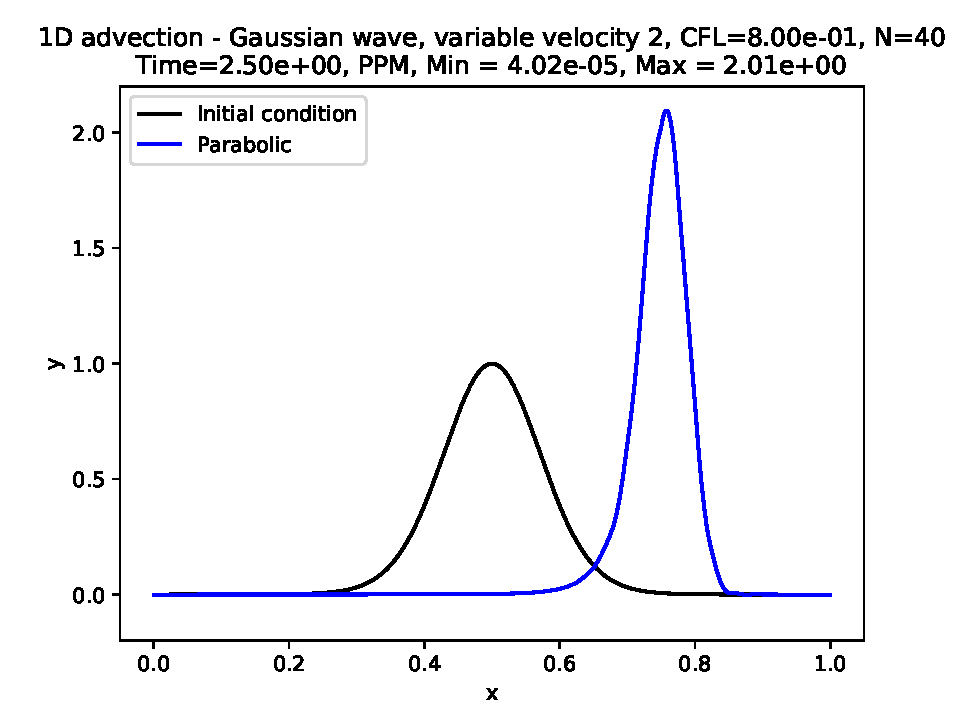
\includegraphics[width=1\linewidth]{1d_adv_tc2_ic2_vf3_t24_N40_PPM}
			\caption{PPM.\label{chp2-sec-exp-adv5-a}}
  \end{subfigure}
  \begin{subfigure}{0.49\textwidth}
    \centering
			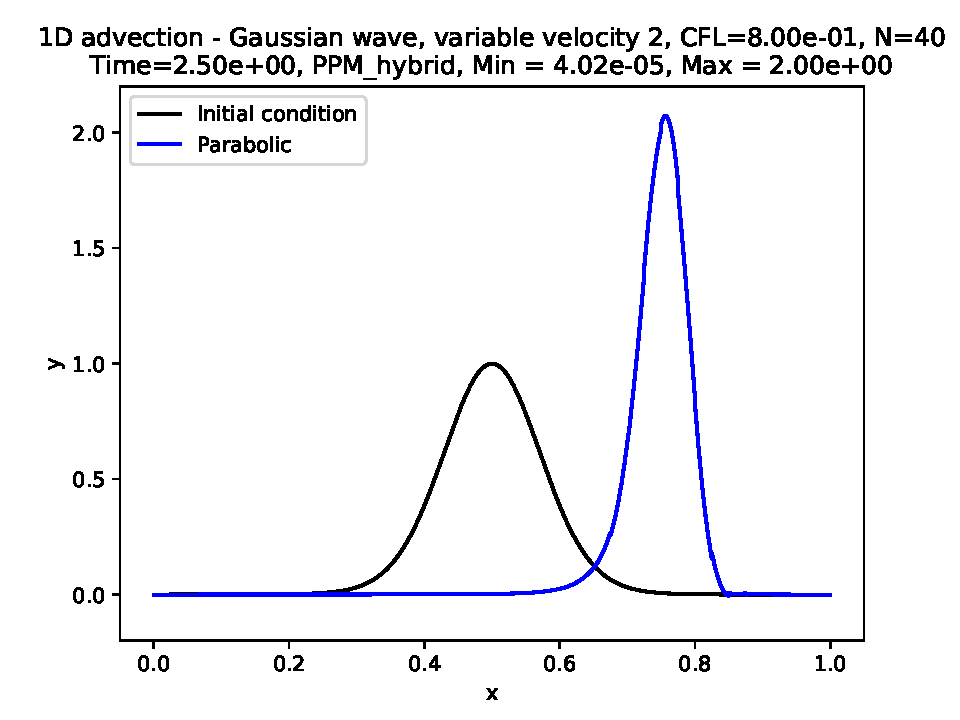
\includegraphics[width=1\linewidth]{1d_adv_tc2_ic2_vf3_t24_N40_PPM_hybrid}
			\caption{Hybrid PPM.\label{chp2-sec-exp-adv5-b}}
  \end{subfigure}

  \begin{subfigure}{0.49\textwidth}
    \centering
		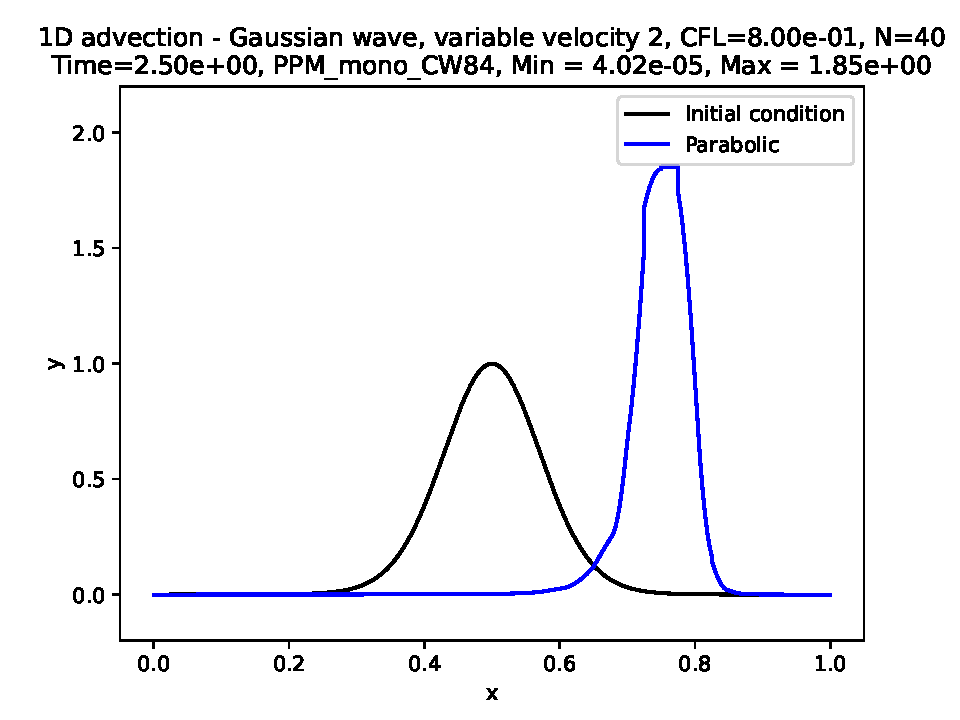
\includegraphics[width=1\linewidth]{1d_adv_tc2_ic2_vf3_t24_N40_PPM_mono_CW84}
    \caption{PPM + CW84 monotonization.\label{chp2-sec-exp-adv5-c}}
  \end{subfigure}
  \begin{subfigure}{0.49\textwidth}
    \centering
			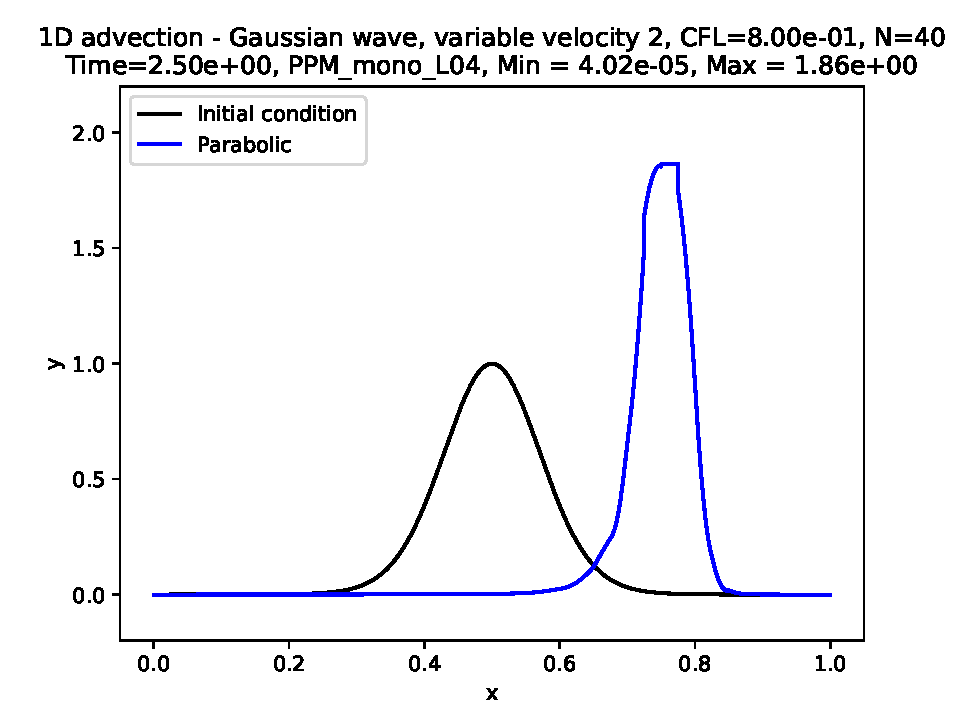
\includegraphics[width=1\linewidth]{1d_adv_tc2_ic2_vf3_t24_N40_PPM_mono_L04}
      \caption{PPM + L04 monotonization.\label{chp2-sec-exp-adv5-d}}
  \end{subfigure} 

  \begin{subfigure}{0.49\textwidth}
    \centering
			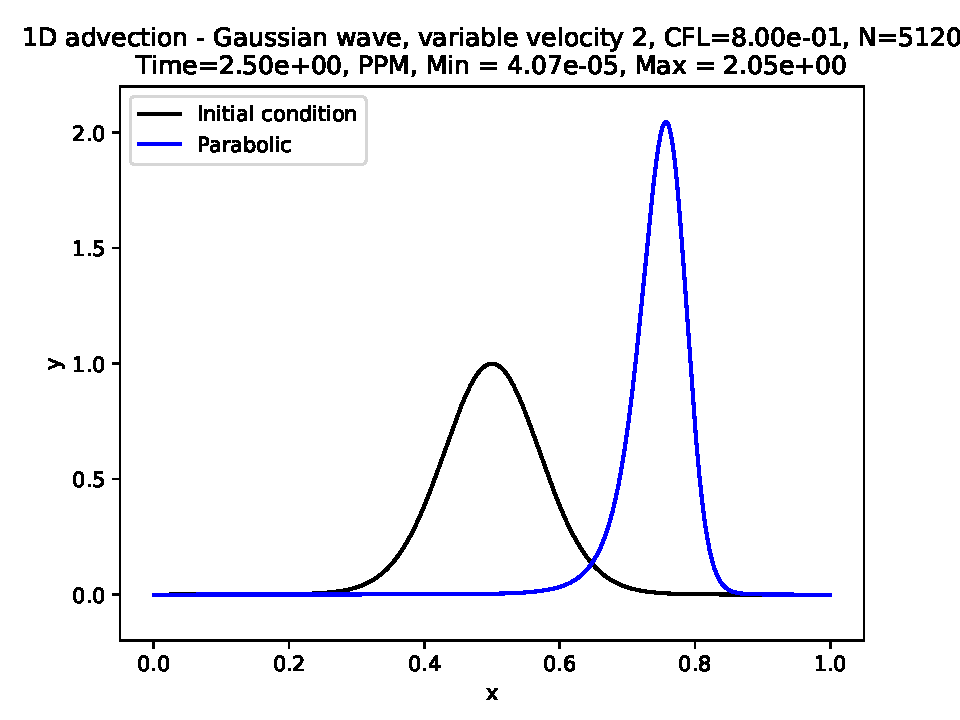
\includegraphics[width=1\linewidth]{1d_adv_tc2_ic2_vf3_t3199_N5120_PPM}
      \caption{Reference solution.\label{chp2-sec-exp-adv5-e}}
  \end{subfigure} 
	\caption{ Similar to Figure \ref{chp2-sec-exp-adv1} but using $N=40$, 
	the initial condition given by Equation \eqref{chp2-ic2}, the variable velocity given by Equation
	\eqref{chp2-vel2} and the final time is 2.5 (half a period). In (e) we show a reference solution, using the PPM scheme with 
	5120 cells. \label{chp2-sec-exp-adv5}}
\end{figure}

\newpage


\begin{figure}[!htb]
  \centering
  \begin{subfigure}{0.49\textwidth}
    \centering
			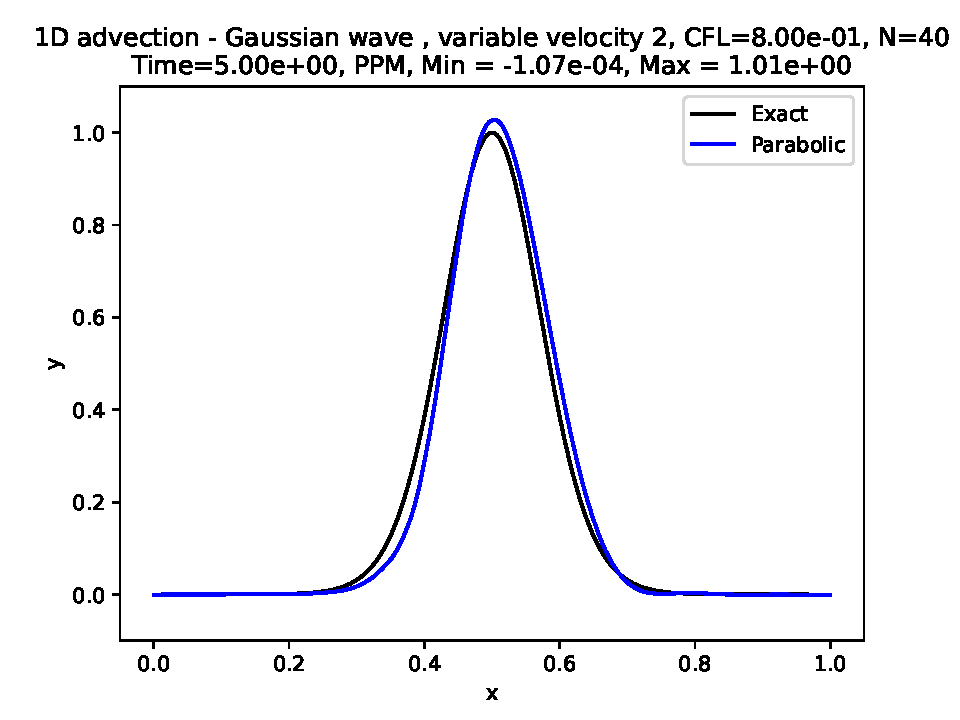
\includegraphics[width=1\linewidth]{1d_adv_tc2_ic2_vf3_t49_N40_PPM}
			\caption{PPM.\label{chp2-sec-exp-adv6-a}}
  \end{subfigure}
  \begin{subfigure}{0.49\textwidth}
    \centering
			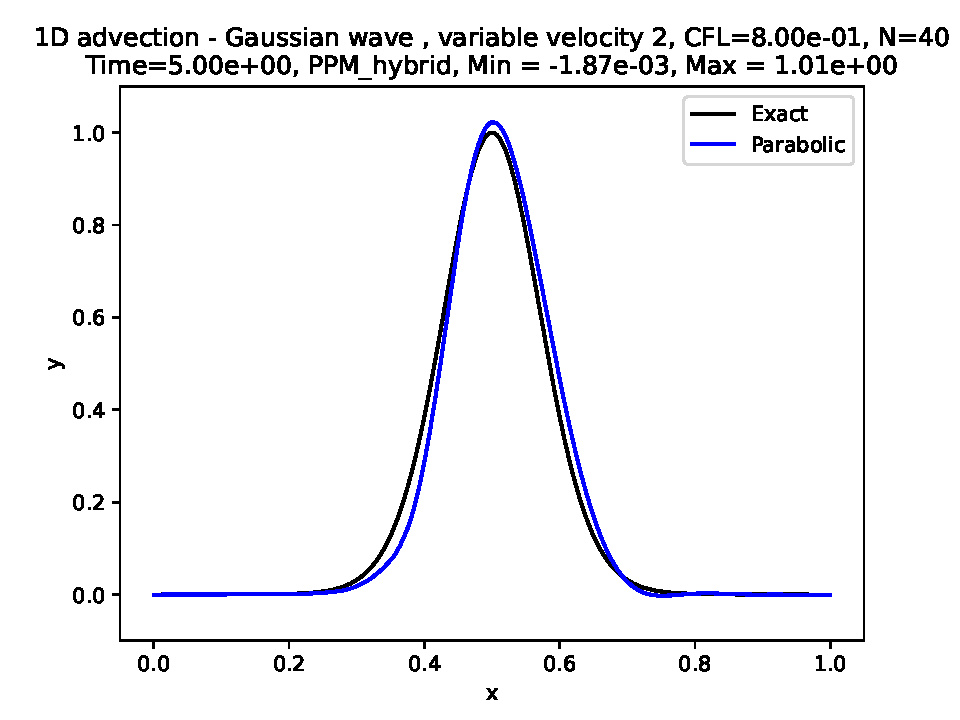
\includegraphics[width=1\linewidth]{1d_adv_tc2_ic2_vf3_t49_N40_PPM_hybrid}
			\caption{Hybrid PPM.\label{chp2-sec-exp-adv6-b}}
  \end{subfigure}

  \begin{subfigure}{0.49\textwidth}
    \centering
		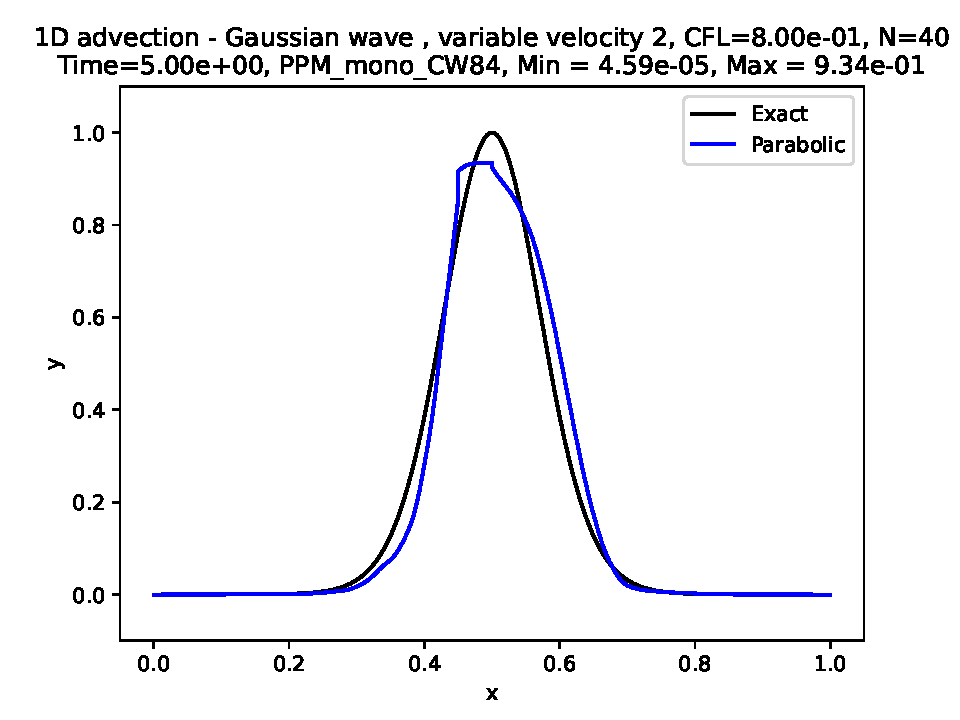
\includegraphics[width=1\linewidth]{1d_adv_tc2_ic2_vf3_t49_N40_PPM_mono_CW84}
    \caption{PPM + CW84 monotonization.\label{chp2-sec-exp-adv6-c}}
  \end{subfigure}
  \begin{subfigure}{0.49\textwidth}
    \centering
			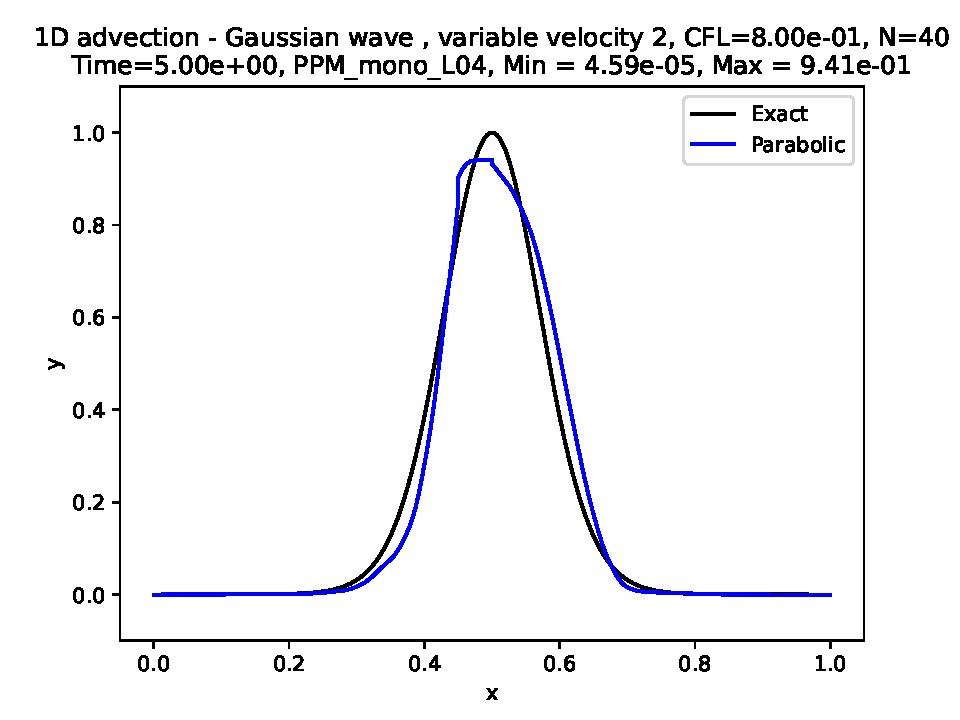
\includegraphics[width=1\linewidth]{1d_adv_tc2_ic2_vf3_t49_N40_PPM_mono_L04}
      \caption{PPM + L04 monotonization.\label{chp2-sec-exp-adv6-d}}
  \end{subfigure} 
	\caption{ Similar to Figure \ref{chp2-sec-exp-adv2} but using $N=40$, 
	the initial condition given by Equation \eqref{chp2-ic2} and the variable velocity given by Equation
	\eqref{chp2-vel2} \label{chp2-sec-exp-adv6}.}
\end{figure}

\begin{figure}[!htb]
  \centering
  \begin{subfigure}{0.49\textwidth}
    \centering
		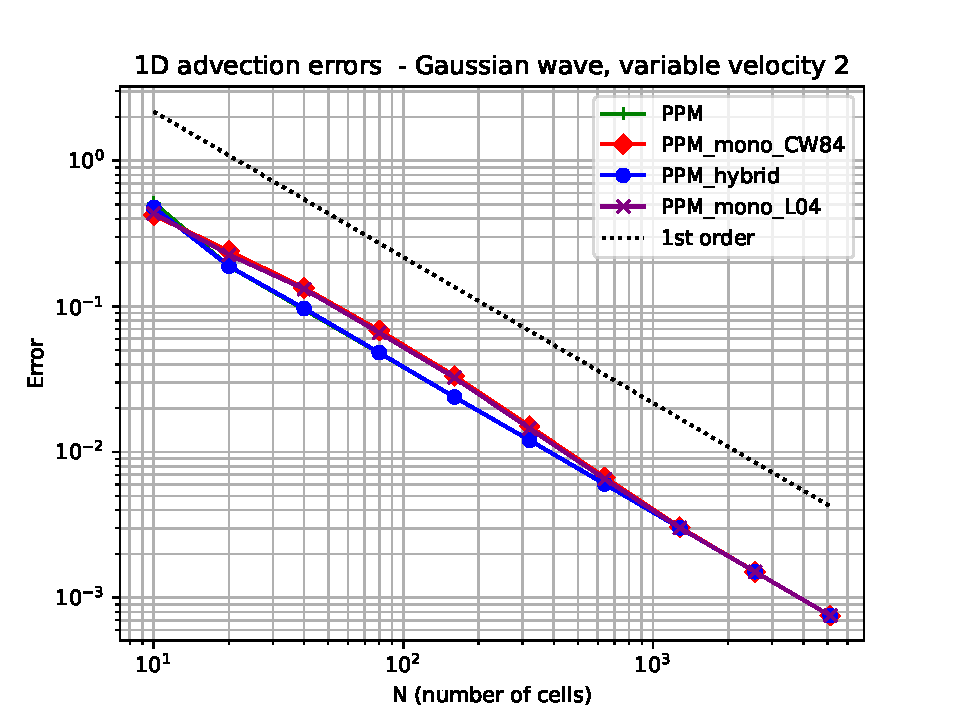
\includegraphics[width=1\linewidth]{1d_adv_tc2_ic2_vf3_parabola_errors}
		\caption{Error.\label{chp2-sec-exp-adv6-error}}
  \end{subfigure}
  \begin{subfigure}{0.49\textwidth}
    \centering
			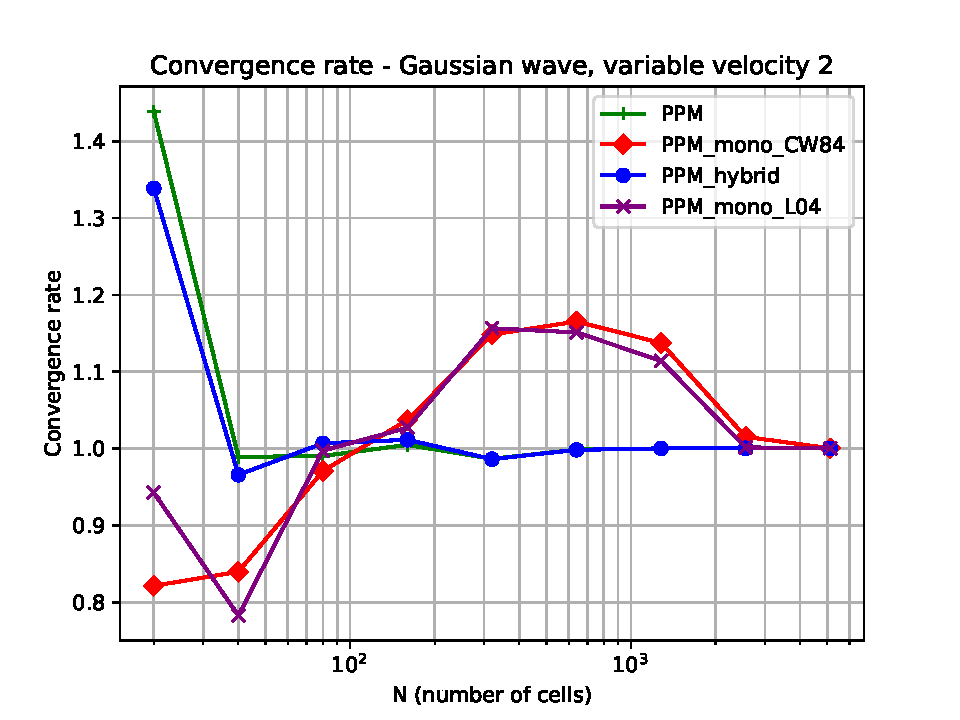
\includegraphics[width=1\linewidth]{1d_adv_tc2_ic2_vf3_convergence_rate}
		\caption{Convergence rate.\label{chp2-sec-exp-adv6-CR}}
  \end{subfigure}
	\caption{ Similar to Figure \ref{chp2-sec-exp-adv1-2} but using
	the initial condition given by Equation	\eqref{chp2-ic2} and the variable 
	velocity given by Equation \eqref{chp2-vel2}.\label{chp2-sec-exp-adv6-2}}
\end{figure}

\newpage
\section{Concluding remarks}
\label{chp2-sec-conclusion}
